\documentclass[10pt,]{book}

% Packages I added.
\usepackage{placeins}
\usepackage{caption}
\usepackage{float}
\usepackage{flafter}
\usepackage{makeidx}
\usepackage[nottoc]{tocbibind}
\usepackage{fancyhdr}
\usepackage{xcolor}
\usepackage{framed}
\usepackage{tocloft}
% End of packages I added.

\usepackage[T1]{fontenc}
\usepackage{lmodern}
\usepackage{amssymb,amsmath}
\usepackage{ifxetex,ifluatex}
\usepackage{fixltx2e} % provides \textsubscript
% use upquote if available, for straight quotes in verbatim environments
\IfFileExists{upquote.sty}{\usepackage{upquote}}{}
\ifnum 0\ifxetex 1\fi\ifluatex 1\fi=0 % if pdftex
  \usepackage[utf8]{inputenc}
\else % if luatex or xelatex
  \ifxetex
    \usepackage{mathspec}
    \usepackage{xltxtra,xunicode}
  \else
    \usepackage{fontspec}
  \fi
  \defaultfontfeatures{Mapping=tex-text,Scale=MatchLowercase}
  \newcommand{\euro}{€}
    \setmainfont{DejaVu Serif}
    \setsansfont{DejaVu Sans}
    \setmonofont[Mapping=tex-ansi]{Ubuntu Mono}
\fi
% use microtype if available
\IfFileExists{microtype.sty}{\usepackage{microtype}}{}
\usepackage[margin=1in, paperwidth=7in, paperheight=9in]{geometry}
\usepackage{graphicx}
% Redefine \includegraphics so that, unless explicit options are
% given, the image width will not exceed the width of the page.
% Images get their normal width if they fit onto the page, but
% are scaled down if they would overflow the margins.
\makeatletter
% Fix TOC overflow.
\renewcommand{\@pnumwidth}{3em} 
\renewcommand{\@tocrmarg}{4em}
% End fix TOC overflow.
\def\ScaleIfNeeded{%
  \ifdim\Gin@nat@width>\linewidth
    \linewidth
  \else
    \Gin@nat@width
  \fi
}
\makeatother
\let\Oldincludegraphics\includegraphics
{%
 \catcode`\@=11\relax%
 \gdef\includegraphics{\@ifnextchar[{\Oldincludegraphics}{\Oldincludegraphics[width=\ScaleIfNeeded]}}%
}%
\ifxetex
  \usepackage[setpagesize=false, % page size defined by xetex
              unicode=false, % unicode breaks when used with xetex
              xetex]{hyperref}
\else
  \usepackage[unicode=true]{hyperref}
\fi
\hypersetup{breaklinks=true,
            bookmarks=true,
            pdfauthor={Jim Lehmer},
            pdftitle={Jim's Ten Steps to Linux Survival},
            colorlinks=true,
            citecolor=black,
            urlcolor=black,
            linkcolor=black,
            pdfborder={0 0 0}}
\urlstyle{same}  % don't use monospace font for urls
% Make links footnotes instead of hotlinks:
\renewcommand{\href}[2]{#2\footnote{\url{#1}}}
\usepackage[normalem]{ulem}
% avoid problems with \sout in headers with hyperref:
\pdfstringdefDisableCommands{\renewcommand{\sout}{}}
\setlength{\parindent}{0pt}
\setlength{\parskip}{6pt plus 2pt minus 1pt}
\setlength{\emergencystretch}{3em}  % prevent overfull lines
\setcounter{secnumdepth}{0}

\title{Jim's Ten Steps to Linux Survival}
\author{Jim Lehmer}
\date{2015}

% Overriding commands.
\makeindex
\restylefloat{figure}
\floatplacement{figure}{H}
% Originals from http://www-rohan.sdsu.edu/~aty/bibliog/latex/floats.html
% General parameters, for ALL pages:
\renewcommand{\topfraction}{0.7}	  % max fraction of floats at top
\renewcommand{\bottomfraction}{0.7}	% max fraction of floats at bottom
\renewcommand{\textfraction}{0.3}	  % allow minimal text w. figs
% Parameters for TEXT pages (not float pages):
\setcounter{topnumber}{2}
\setcounter{bottomnumber}{2}
\setcounter{totalnumber}{2}         % 2 may work better
% Parameters for FLOAT pages (not text pages):
% N.B.: floatpagefraction MUST be less than topfraction !!
\renewcommand{\floatpagefraction}{0.65}	% require fuller float pages
% Parameters for double-column pages:
\renewcommand{\dbltopfraction}{0.9}	% fit big float above 2-col. text
\renewcommand{\dblfloatpagefraction}{0.7}	% require fuller float pages
\setcounter{dbltopnumber}{2}        % for 2-column pages
\overfullrule=2cm   % Black bars to show overfull boxes
\renewcommand{\chaptername}{Step}
\renewcommand{\contentsname}{Steps}
\numberwithin{figure}{chapter}
\DeclareRobustCommand{\drcap}[1]{\begin{figure}[H]\caption{#1}\end{figure}}
\DeclareRobustCommand{\drcmd}[1]{\index{Commands!#1}}
\DeclareRobustCommand{\drenv}[1]{\index{Environment Variables!#1}}
\DeclareRobustCommand{\drios}[1]{\index{OS and OS-Like Substances!#1}}
\DeclareRobustCommand{\drshl}[1]{\index{Shells!#1}}
\DeclareRobustCommand{\drvic}[2]{\index{vi Commands!#1 (#2)}}
% End of overriding commands.

\begin{document}
\setlength{\cftfignumwidth}{4em}
\pagestyle{empty}

\maketitle

{
\hypersetup{linkcolor=black}
\setcounter{tocdepth}{3}
\tableofcontents
}

% Add list of figures.
{
\listoffigures
\vfill
}
% End of list of figures.

\setcounter{chapter}{-2}

\cleardoublepage
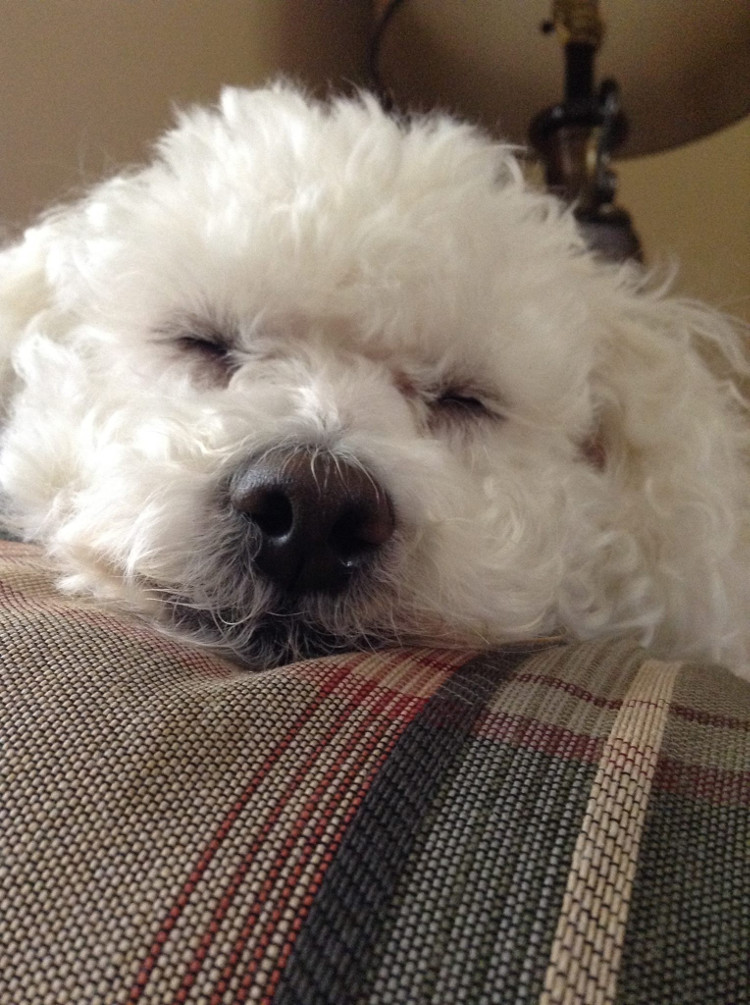
\includegraphics{./images/Merv.jpg}~\\ Merv sez, "Don't panic."
\clearpage
~\\\hspace*{0.333em}\\ By James Lehmer ~\\\hspace*{0.333em}\\ v0.7
~\\\hspace*{0.333em}\\

\includegraphics{./images/cc-by-sa.png}\\\emph{Jim's Ten Steps to Linux
Survival} by James Lehmer is licensed under a
\href{http://creativecommons.org/licenses/by-sa/4.0/}{Creative Commons
Attribution-ShareAlike 4.0 International License}.
~\\\hspace*{0.333em}\\ \textbf{Dedicated to my first three technical
mentors} - Jim Proffer, who taught me digging deeper was fun and let me
do so (often in production). Jerry Wood, who taught me to stop and think
(and once called me an "inveterate toolmaker" in a review). And Kim
Manchak, who let me be more than he hired me to be (and continues to be
a great chess opponent). Thank you, gentlemen. I've tried to pay it
forward. This book is part of that.

\pagestyle{fancy} \fancyhead{}
\fancyhead[LE]{\slshape JIM'S\ TEN\ STEPS\ TO\ LINUX\ SURVIVAL}
\fancyhead[RO]{\slshape \leftmark} \renewcommand{\headrulewidth}{0.4pt}

\hyperdef{}{introduction}{\chapter{Introduction}\label{introduction}}

\begin{quote}
\emph{"And you may ask yourself, 'Well, how did I get here?'"} - Talking
Heads (\emph{Once in a Lifetime})
\end{quote}

This is my little "Linux and Bash in 10 steps" guide. It's based around
what I consider the essentials for \sout{floundering around} acting like
I know what I'm doing in Linux, BSD and "UNIX-flavored" systems and
looking impressive among people who have only worked on Windows in the
GUI. Your "10 steps" may be different than mine and that's fine, but
this list is mine.

I said ten things, but I lied, because history is really important, so
we will start at step \#0. And since this is before even that I guess
that means this is a 12-step program...

Here is what we'll cover in the rest of this book:

\begin{enumerate}
\def\labelenumi{\arabic{enumi}.}
\setcounter{enumi}{-1}
\item
  \hyperref[some-history]{\textbf{Some History}} – UNIX vs. BSD, System
  V vs. BSD, Linux vs. BSD, POSIX, “UNIX-like,” Cygwin, and why any of
  this matters now, “Why does this script off the internet work on this
  system and not on that one?”
\item
  \hyperref[come-out-of-your-shell]{\textbf{Come Out of Your Shell}} –
  \texttt{sh} vs. \texttt{ash} vs. \texttt{bash} vs. everything else,
  "REPL”, interactive vs. scripts, command history, tab expansion,
  environment variables and "A path! A path!"
\item
  \hyperref[file-under-directories]{\textbf{File Under "Directories"}} –
  \texttt{ls}, \texttt{mv}, \texttt{cp}, \texttt{rm} (\texttt{-rf *}),
  \texttt{cat}, \texttt{chmod}/\texttt{chgrp}/\texttt{chown} and
  everyone's favorite, \texttt{touch}.
\item
  \hyperref[finding-meaning]{\textbf{Finding Meaning}} – the
  \texttt{find} command in all its glory. Probably the single most
  useful command in "UNIX" (I think).
\item
  \hyperref[grokking-grep]{\textbf{Grokking \texttt{grep}}} – and
  probably gawking at \texttt{awk} while we are at it, which means
  regular expressions, too. Now we have two problems.
\item
  \hyperref[just-a-series-of-pipes]{\textbf{“Just a Series of Pipes”}} –
  \texttt{stdin}/\texttt{stdout}/\texttt{stderr}, redirects, piping
  between commands.
\item
  \hyperref[vi]{\textbf{\texttt{vi}}} (had to be \#6, if you think about
  it) – how to stay sane for 10 minutes in \texttt{vi}. Navigation,
  basic editing, find, change/change-all, cut and paste, undo, saving
  and canceling. Plus easier alternatives like \texttt{nano}, and why
  \texttt{vi} still matters.
\item
  \hyperref[the-whole-wide-world]{\textbf{The Whole Wide World}} –
  \texttt{curl}, \texttt{wget}, \texttt{ifconfig}, \texttt{ping},
  \texttt{ssh}, \texttt{telnet}, \texttt{/etc/hosts} and email before
  Outlook.
\item
  \hyperref[the-man-behind-the-curtain]{\textbf{The Man Behind the
  Curtain}} - \texttt{/proc}, \texttt{/dev}, \texttt{ps},
  \texttt{/var/log}, \texttt{/tmp} and other things under the covers.
\item
  \hyperref[how-do-you-know-what-you-dont-know-man]{\textbf{How Do You
  Know What You Don’t Know, \texttt{man}?}} – \texttt{man},
  \texttt{info}, \texttt{apropos}, Linux Documentation Project, Debian
  and Arch guides, StackOverflow and the dangers of searching for
  “\texttt{man find}” or “\texttt{man touch}” on the internet.
\item
  \hyperref[and-so-on]{\textbf{And So On}} - \texttt{/etc}, starting and
  stopping services, \texttt{apt-get}/\texttt{rpm}/\texttt{yum}, and
  more.
\end{enumerate}

Plus \hyperref[appendices]{some stuff} at the end to tie the whole room
together.

\section*{Batteries Not Included}\label{batteries-not-included}
\addcontentsline{toc}{section}{Batteries Not Included}

It should be obvious that there is \textbf{\emph{plenty}} that is not
covered:

\begin{itemize}
\item
  \textbf{System initialization} - besides, the whole "UNIX" world is in
  flux right now over system initialization architecture and the shift
  from \href{https://en.wikipedia.org/wiki/Init}{"init"} scripts to
  \href{https://en.wikipedia.org/wiki/Systemd}{\texttt{systemd}}.
\item
  \textbf{Scripting logic} - scripting, logic constructs
  (\texttt{if}/\texttt{fi}, \texttt{while}/\texttt{done}, and the like).
\item
  \textbf{Desktops} - X Windows and the plethora of desktop environments
  like GNOME, KDE, Cinnamon, Mate, Unity and on and on. This is where
  "UNIX" systems get the farthest apart in terms of interoperability,
  settings and customization.
\item
  \textbf{Servers} - setting up or configuring web servers like Apache
  or node, email servers like dovecot, Samba servers for file shares,
  and so on.
\item
  \textbf{Security} - other than the simple basics of the file system
  security model.
\end{itemize}

Plus so much more. Again, this is not meant to be exhaustive, but to
help someone whose system administration experience has been limited to
"Next-Next-Next-Finish" installs and filling in text boxes in wizards on
Windows.

\section*{Please, Give Generously}\label{please-give-generously}
\addcontentsline{toc}{section}{Please, Give Generously}

That said, if you find something amiss in here - a typo, a misconception
or mistake, or a command or parameter you \textbf{\emph{really, really,
really}} think should be in here even though I said I am not trying to
be exhaustive, feel free to
\href{https://github.com/dullroar/ten-steps-to-linux-survival}{clone it
from GitHub}, make your changes and send me a \texttt{git pull} request.
Or you can try to
\href{https://github.com/dullroar/ten-steps-to-linux-survival/issues}{file
it as an issue} and I'll see how I feel that day.

\section*{Why?}\label{why}
\addcontentsline{toc}{section}{Why?}

Because I work in a primarily Windows-oriented shop, and I seem to be
"the guy" that everyone comes to when they need help on a Linux or
related system. I don't count myself a Linux guru (\textbf{\emph{at
all}}), but I have been running it since 1996 (Slackware on a laptop
with 8MB of memory!), and have worked on or run at home various ports
and flavors and and versions and distros of "UNIX" over the years,
including:

\begin{itemize}
\item
  \textbf{AIX}
\item
  \textbf{FreeBSD}
\item
  \textbf{HP/UX}
\item
  \textbf{Linux} - literally more distros than I can count or remember,
  but at least Debian, Fedora, Yellow Dog, Ubuntu/Kubuntu/Xubuntu, Mint,
  Raspbian, Gentoo, Red Hat and of course the venerable Slackware.
\item
  \textbf{Solaris}
\item
  \textbf{SunOS}
\end{itemize}

...on various machines and machine architectures from mighty Sun servers
to generic "Intel" VMs down to Raspberry Pis (plus an original "wedge"
iMac running as a kitchen kiosk long after its "Best by" date and OS/9's
demise, thanks to Yellow Dog Linux).

All that while also working on MVS, VSE, OS/2, DOS since 3.x, Windows
since 1.x, etc., etc. I don't think I am special when I list all that -
there are lots of people with my level of experience \textbf{\emph{and
better}}, especially in commercial software engineering. I am just one
of them.

But for some reason there are many places, especially in small and
medium business (SMB) environments, where the "stack" tends to be more
purely Microsoft because it keeps things simpler and cheaper for the
(smaller) staff. I work in such a place. The technical staff is quite
competent, but when they bump up against systems whose primary "user
interface" for system administration is a command prompt and some
scripts, they panic.

This is my attempt to help my co-workers by saying:

\begin{quote}
\emph{"Don't panic."} - Douglas Adams (\emph{Hitchhiker's Guide to the
Galaxy})
\end{quote}

It started out as a proposal I made a while ago to develop a "lunch and
learn" session of about 60-90 minutes of what I considered to be "a
Linux survival guide." The list in the
\hyperref[introduction]{\emph{Introduction}} above is based on my
original email proposal. The audience would be entirely technical,
primarily "IT" (Windows/Cisco/VMWare/Exchange/SAN admins).

My goal is not to get into scripting or system setup and hardening or
the thousand different ways to slice a file. Instead, the scenario I see
in my head is for one of the participants in that "lunch and learn,"
armed with that discussion and having glanced through this book, to be
better able to survive if dropped into the jungle with:

\begin{quote}
\emph{"The main www site is down, and all the people who know about it
are \textgreater{} out. It's running on some sort of Linux, I think, and
the credentials and \textgreater{} IP address are scrawled on this
sticky note. Can you get in and poke \textgreater{} around and see if
you can figure it out?"} - your boss (next Tuesday \textgreater{}
morning)
\end{quote}

Well, as I started to type out my notes of what I considered to be
"essential," they just kept growing and growing. And now, some nights,
weekends and lunch hours gone, this is what you see as the result. I
figure the slides will be easier to prepare for that "lunch and learn,"
now that I have the "notes"!

\section*{Caveat Administrator}\label{caveat-administrator}
\addcontentsline{toc}{section}{Caveat Administrator}

Even so, anything like this is incomplete. Anyone knowledgable of Linux
will probably splutter their coffee into their neckbeard at least once a
chapter because I don't mention a parameter on a command or an entire
subject at all! And that's right - because this "survival guide" is
already long enough.

This book is not meant to be an authoritative source, but instead a
\href{https://en.wikipedia.org/wiki/Fake_book}{"fake book"} for getting
up and running \textbf{\emph{quickly}} with the sheer basics, plus
knowing where to go for help. I modeled it explicitly after "short and
opinionated" tech books such as Douglas Crockford's
\href{http://shop.oreilly.com/product/9780596517748.do}{\emph{Javascript:
The Good Parts}} or Zed Shaw's
\href{http://learnpythonthehardway.org/}{\emph{Learn Python the Hard
Way}}. If you like those big, thick tech books that are measured by the
kilogram, this is not the book for you.

It is also not a replacement for reading the real documentation and
doing research and testing, especially in production! But hopefully it
will help get you through that "Can you get in and poke around and see
if you can figure it out?" scenario, above. And if Linux should start
becoming more of your job, maybe this will help as a gentle push toward
"RTFM" along with thinking in "The UNIX Way."

\textbf{WARNING:} \textbf{\emph{Many of the commands in this book can
alter your system and possibly damage it.}} Obvious candidates include
the file system commands like \texttt{rm}, the \texttt{vi} editor
(obviously), and some of the "system admin" commands mentioned later,
including system and service restarts. Use your common sense plus the
various resources for documentation mentioned in this book to make sure
you aren't doing anything destructive to your system, especially in
production. \textbf{\emph{You have been warned!}}

\section*{Conventions}\label{conventions}
\addcontentsline{toc}{section}{Conventions}

If a command, file name or other "computer code" is shown in-line in a
sentence, it will appear in a fixed-width font, e.g.,
\texttt{ls -{}-recursive *.txt}.

If a command and its output, script code or something else is shown in a
block, it will appear like this:

\drcap{Code snippet}

\begin{verbatim}
~ $ ps -AH
  PID TTY          TIME CMD
    2 ?        00:00:00 kthreadd
    3 ?        00:00:00   ksoftirqd/0
    5 ?        00:00:00   kworker/0:0H
    7 ?        00:00:19   rcu_sched
    8 ?        00:00:04   rcuos/0
    9 ?        00:00:09   rcuos/1
   10 ?        00:00:07   rcuos/2
...and so on...
\end{verbatim}

\textbf{Note:} The examples in this book typically show something like
\texttt{\textasciitilde{} \$} before the command, or \texttt{\#} (when
logged in as root) or \texttt{\%} (when running under \texttt{csh}).
These "command prompts" are set in \texttt{bash} via the
\href{https://www.linux.com/learn/docs/ldp/443-bash-prompt-howto}{\texttt{PS1}
environment variable}\drenv{PS1} and are not meant to be typed in as
part of the command.

\section*{Acknowledgments}\label{acknowledgments}
\addcontentsline{toc}{section}{Acknowledgments}

Thanks to Ken Astl for reading an early draft of this book.

\hyperdef{}{some-history}{\chapter{Some History}\label{some-history}}

\textbf{\emph{UNIX vs. BSD, System V vs. BSD, Linux vs. BSD, POSIX,
“UNIX-like,” Cygwin, and why any of this matters now. “Why does this
script off the internet work on this system and not on that one?”}}

\begin{quote}
\emph{"That men do not learn very much from the lessons of history is
the most important of all the lessons of history."} - Aldous Huxley
\end{quote}

UNIX and its successors such as Linux have a long history reaching into
the depths of time:

\begin{itemize}
\item
  \textbf{Prehistory} - late 1960s, Nixon, Vietnam, Woodstock, Moon
  landing, \href{https://en.wikipedia.org/wiki/Multics}{Multics} at MIT,
  GE and Bell Labs.
\item
  \textbf{In the beginning} - early 1970s, Nixon drags on, Watergate,
  Bell Labs, \href{https://en.wikipedia.org/wiki/Ken_Thompson}{Thompson}
  \& \href{https://en.wikipedia.org/wiki/Dennis_Ritchie}{Ritchie},
  \href{https://en.wikipedia.org/wiki/History_of_Unix}{UNIX}\drios{UNIX},
  blah blah blah...
\item
  \textbf{More Trouble From Berkeley} - late 1970s, Carter, disco, Iran
  hostages, UC Berkely releases the
  \href{https://en.wikipedia.org/wiki/Berkeley_Software_Distribution}{Berkeley
  Software Distribution} (BSD)\drios{BSD}, a port based on the Bell Labs
  UNIX. Let the forking begin!
\item
  \textbf{Goes commercial} - 1980s, Reagan, Iran Contra, \emph{E.T.},
  AT\&T releases
  \href{https://en.wikipedia.org/wiki/UNIX_System_V}{System
  V}\drios{System V} as first commercial UNIX. From the same background
  as Bell Labs UNIX, but evolved with subtle and not so subtle
  differences in approaches to command syntax, networking and much more.
  It is this release and AT\&T's copyrights that are the basis of all
  the SCO-vs-Linux lawsuits 2-3 decades later.
\item
  \textbf{Explosion of "UNIX"} -late 1980s/early 1990s, Bush I, Berlin
  Wall falls, Gulf War I, proliferation of proprietary (and different)
  "UNIX" platforms:

  \begin{itemize}
  \itemsep1pt\parskip0pt\parsep0pt
  \item
    \textbf{HP HP-UX}
  \item
    \textbf{Sun SunOS} - BSD flavor.
  \item
    \textbf{Sun Solaris} - System V flavor. Now Oracle Solaris.
  \item
    \textbf{IBM AIX}
  \item
    \textbf{SGI IRIX}
  \item
    \textbf{...and many, many more!} - although mostly all that's left
    now is HP-UX, AIX and Solaris.
  \end{itemize}
\item
  \textbf{Linux} - 1991+, Clinton I, grunge, \emph{Titanic},
  \href{https://en.wikipedia.org/wiki/Linus_Torvalds}{Linus Torvalds}
  releases a project called
  \href{https://en.wikipedia.org/wiki/Linux}{Linux}\drios{Linux} based
  on \href{https://en.wikipedia.org/wiki/MINIX}{MINIX}\drios{MINIX} (and
  hence why Linus says Linux is pronounced like "MINIX" and not like
  "Linus").
\item
  \textbf{Proliferation of the BSDs} - mid-to-late 1990s, still Clinton
  I, Monicagate, Kosovo, various ports of BSD including
  \href{https://en.wikipedia.org/wiki/NetBSD}{NetBSD}\drios{NetBSD},
  \href{https://en.wikipedia.org/wiki/FreeBSD}{FreeBSD}\drios{FreeBSD}
  and
  \href{https://en.wikipedia.org/wiki/OpenBSD}{OpenBSD}\drios{OpenBSD},
  all happen in the same time frame as Linux. Like Linux distros, each
  has its own focus and prejudices, some of which are distinctly
  "anti-Linux." The "big three" are all still in heavy use today,
  especially among ISPs. The perception is still out there among a
  generation of sysadmins that Linux is for the desktop and BSDs for
  servers, but that reality shifted a long time ago.
\item
  \textbf{Ports of call} - 2000+, Bush II \& Obama, Afghanistan \& Gulf
  War 2, lots of cross-porting of everything open source. However,
  \href{https://en.wikipedia.org/wiki/Open-source_license}{licenses
  matter}, and
  \href{https://en.wikipedia.org/wiki/Comparison_of_free_and_open-source_software_licenses}{there
  sure are a lot of them}. While it has settled down some with the
  dismissal of the SCO lawsuit, intellectual property remains a problem
  area in open source, even as its use has exploded.
\end{itemize}

\textbf{Q:} So, what's Linux? Or BSD? Or even UNIX?

\textbf{A:} Depends on who you're asking and in what context!

Hence, for the rest of this text I will tend to talk somewhat
interchangeably about "Linux" and "UNIX" and the like. When it matters,
I will mention which OS I am discussing by name, but often I will use
"UNIX" (in quotes) to mean anything in the "family tree" of the original
Bell Labs offspring, or that "acts like," well, UNIX.

To further muddy the waters, there have been multiple attempts to
"standardize" whatever it is this thing is called:

\begin{itemize}
\itemsep1pt\parskip0pt\parsep0pt
\item
  \href{https://en.wikipedia.org/wiki/POSIX}{\textbf{POSIX}}\drios{POSIX}
  - a de jure set of standards created in the 1980s and 1990s to try to
  bring order to the chaos that was commercial UNIX-flavored operating
  systems of the time. It worked. Sorta. Especially once the US
  government started wanting systems to be "POSIX-compliant."
\end{itemize}

\textbf{Note:} No system runs POSIX, they all are "similar but
different." Even Windows can claim to be POSIX in some respects (and has
an installable POSIX subsystem), but that doesn't mean POSIX-compliant
code will run there unchanged.

\begin{itemize}
\item
  \href{https://en.wikipedia.org/wiki/GNU_Project}{\textbf{GNU
  Project}}\drios{GNU} -
  \href{https://en.wikipedia.org/wiki/Richard_Stallman}{Richard
  Stallman} founded the
  \href{https://en.wikipedia.org/wiki/Free_Software_Foundation}{Free
  Software Foundation} (FSF) and GNU project in the mid-1980s,
  \textbf{\emph{long}} before Linux (GNU = "GNU's Not Unix"). The GNU
  project delivers \href{https://www.gnu.org/software/software.html}{a
  suite of programs and tools}, many of which are used in both Linux and
  BSD variants as de facto standards.
\item
  \textbf{Various Linux Efforts} - there have also been various
  movements over the years, some more successful than others, to
  "standardize" Linux or some part of it, such as the file system
  layout, the \texttt{init} system, documentation, and now even what is
  part of the most basic "core OS" for things like better
  containerization.
\end{itemize}

\section*{Why Does This Matter?}\label{why-does-this-matter}
\addcontentsline{toc}{section}{Why Does This Matter?}

Because there are various "flavors" of commands and tools, based on
whether you're dealing with a System V (Linux) or BSD (Free/Net/Open)
descendant. Some of the OS versions are strong in security, or
networking, or as a desktop. Certain things are "built-in" to the
operating system but most are installed as packages, and depending on
the source of the package it may or may not work correctly on another
"UNIX" system without effort.

It is similar to the history and relationship between
\texttt{COMMAND.EXE}\drshl{COMMAND.EXE} in DOS and
\texttt{CMD.EXE}\drshl{CMD.EXE} in Windows 10, where this would work in
both:

\begin{verbatim}
COPY A.TXT B.TXT
\end{verbatim}

But only the later, network-and-NTFS-aware \texttt{CMD.EXE} could
handle:

\begin{verbatim}
COPY "My 2015 Tax Returns.pdf" \\MyServer\Finances\.
\end{verbatim}

In UNIX-land over time these differences seem to be getting better, but
there are still "gotchas," often involving the differences in open
source licenses in the underlying code. There are fundamental
differences and assumptions between the "GNU" and "GPL" licenses on the
one side and "MIT" and "BSD" licenses on the other. I am not a lawyer,
but I would summarize:

\begin{itemize}
\item
  \textbf{FSF/GNU/GPL} - mostly concerned with keeping open source
  "open," that is sharable and modifiable by all.
\item
  \textbf{BSD \& MIT} - more focused on letting anyone do anything to
  the code as long as the original author is acknowledged and liability
  released.
\end{itemize}

The best thing is to be vaguely aware of this history and licenses and
if something isn't available on a certain platform or if a command isn't
taking a specific parameter to search for variants.

For example, note the difference in output between showing all processes
with the \href{http://linux.die.net/man/1/ps}{\texttt{ps}}\drcmd{ps}
(\emph{process}) command on a Linux system, in this case Linux Mint
under \texttt{bash}\drshl{bash}:

\drcap{ps on Linux in bash}

\begin{verbatim}
~ $ ps -a
  PID TTY          TIME CMD
 4508 pts/3    00:00:00 su
 4516 pts/3    00:00:00 bash
 4594 pts/3    00:00:00 ps
\end{verbatim}

...versus on a FreeBSD\drios{FreeBSD} system at my ISP, where
\texttt{csh}\drshl{csh} is the default shell:

\drcap{ps on FreeBSD in csh}

\begin{verbatim}
%ps -a
  PID  TT  STAT      TIME COMMAND
 5073  p0  Ss     0:00.02 -csh (csh)
 5115  p0  RN+    0:00.00 ps -a
\end{verbatim}

To make things even more confusing, the Linux version of \texttt{ps} has
been written to understand the BSD-style syntax and flags, too!

\section*{Panic at the Distro}\label{panic-at-the-distro}
\addcontentsline{toc}{section}{Panic at the Distro}

Remember that "Linux," FreeBSD, OpenBSD and NetBSD are all really just
OS kernels, boot loaders, drivers and enough functionality to get a
computer up and running. Most functionality comes via other "packages."
From almost the beginning there have been alternative approaches to both
what packages should (and should not) be included, as well as how best
to manage the installing, updating and removal of those packages.

In the BSD world each major port has its own approach. In the Linux
world the job of deciding all this and putting it all together falls to
distributions or "distros."\drios{Linux distros} These have evolved over
time into a series of
\href{https://en.wikipedia.org/wiki/Linux_distribution\#Popular_distributions}{"families"}
based in large part around the
\href{https://en.wikipedia.org/wiki/Package_manager}{package management
tool} predominantly used:

\begin{itemize}
\item
  \textbf{\texttt{apt-get}\drcmd{apt-get}, \texttt{dpkg}\drcmd{dpkg} and
  \texttt{.deb} files} -
  \href{https://en.wikipedia.org/wiki/Debian}{Debian}\drios{Debian}
  flavors, such as
  \href{https://en.wikipedia.org/wiki/Ubuntu_\%28operating_system\%29}{Ubuntu}\drios{Ubuntu}
  and \href{https://en.wikipedia.org/wiki/Linux_Mint}{Mint}\drios{Mint}
  (Mint is currently my desktop Linux of choice, Debian my preferred
  server OS, but both solely based on familiarity).
\item
  \textbf{\texttt{pacman}}\drcmd{pacman} -
  \href{https://en.wikipedia.org/wiki/Arch_Linux}{Arch}\drios{Arch}
  flavors.
\item
  \textbf{\texttt{rpm}\drcmd{rpm} and \texttt{yum}\drcmd{yum}} - Red
  Hat\drios{Red Hat} flavors, such as
  \href{https://en.wikipedia.org/wiki/Fedora_\%28operating_system\%29}{Fedora}\drios{Fedora},
  \href{https://en.wikipedia.org/wiki/Red_Hat_Enterprise_Linux}{Red Hat
  Enterprise}\drios{RHEL} and
  \href{https://en.wikipedia.org/wiki/CentOS}{CentOS}\drios{CentOS}.
\item
  \textbf{Source code} -
  \href{https://en.wikipedia.org/wiki/Gentoo_Linux}{Gentoo}\drios{Gentoo}
  tends to be a "compile from scratch" environment, much like
  \href{https://en.wikipedia.org/wiki/FreeBSD_Ports}{FreeBSD}\drios{FreeBSD}.
\item
  \textbf{"Tar balls"} - source code or binaries delivered via archived
  and zipped directories. Common on
  \href{https://en.wikipedia.org/wiki/Slackware}{Slackware}\drios{Slackware},
  some others.
\end{itemize}

\section*{Get Embed With Me}\label{get-embed-with-me}
\addcontentsline{toc}{section}{Get Embed With Me}

A lot of firmware in embedded devices is based on some sort of "UNIX"
flavor. Networking gear at both the consumer and enterprise level,
storage devices and so on all tend to run something that "looks like"
UNIX at some level.
\href{https://en.wikipedia.org/wiki/BusyBox}{BusyBox}\drios{BusyBox}\drshl{BusyBox}
is a good example of a "UNIX-like" shell (command prompt) used by many
embedded systems. Of course, as to what's actually available, who knows?
If you can get shell open, the best thing to do is see what works.

\section*{Cygwin}\label{cygwin}
\addcontentsline{toc}{section}{Cygwin}

\href{http://cygwin.com/}{Cygwin}\drios{Cygwin} is an interesting beast.
It is a DLL for Windows that implements most of the POSIX and related
UNIX-like "system API calls" for programming, and then is also a series
of ported open source packages, including shells, utilities and even
desktop environments, all \textbf{\emph{recompiled}} to run on Windows
as long as the Cygwin DLL is accessible. Like a Linux distro it has an
installer that is a "package manager," and if a package isn't available,
you can usually recompile the source code using Cygwin.

You cannot run Linux or BSD binaries on Cygwin without recompiling them
first. \textbf{However}, you can often run \textbf{\emph{scripts}} from
a Linux environment on Cygwin with little or no tweaking. Which means
you can then take advantage of a lot of excellent open source tools
simply by installing their packages in Cygwin and running scripts
against them.

Ultimately, though, Cygwin is of limited use, basically for getting to
some open source tools on Windows without having to set up a Linux box.
You can do a lot of amazing things with Cygwin with enough effort
(including running X and a desktop environment like GNOME!), but at some
point why not expend that effort in standing up a "real" Linux (virtual)
machine anyway?

\hyperdef{}{come-out-of-your-shell}{\chapter{Come Out of Your
Shell}\label{come-out-of-your-shell}}

\textbf{\emph{\texttt{sh} vs. \texttt{ash} vs. \texttt{bash} vs.
everything else, "REPL”, interactive vs. scripts, command history, tab
expansion, environment variables and "A path! A path!"}}

\begin{quote}
\emph{"If you hold a shell up to your ear, you can hear the OS."} - me
\end{quote}

To avoid getting all pedantic, I am just going to define a shell as an
environment in which you can execute commands. People tend to think of a
shell as a "command prompt," but you can run a shell without running a
command prompt, but not vice versa - an interactive command prompt is an
instance of a shell environment almost by definition.

Examples of shells:

\begin{itemize}
\item
  \href{https://technet.microsoft.com/en-us/library/cc754340.aspx}{\textbf{\texttt{CMD.EXE}}}\drshl{CMD.EXE}
  - yes, Windows has a shell.
\item
  \href{https://technet.microsoft.com/en-us/library/ms714469\%28v=VS.85\%29.aspx}{\textbf{\texttt{PowerShell.exe}}}\drshl{Powershell}
  - in fact, it has at least two!
\end{itemize}

In UNIX-land:

\begin{itemize}
\item
  \href{https://en.wikipedia.org/wiki/Bourne_shell}{\textbf{\texttt{sh}}}\drshl{sh}
  - the "original" Bourne shell in UNIX, which spawned:

  \begin{itemize}
  \item
    \href{https://en.wikipedia.org/wiki/Almquist_shell}{\textbf{\texttt{ash}}}\drshl{ash}
    - Almquist shell.

    \begin{itemize}
    \itemsep1pt\parskip0pt\parsep0pt
    \item
      \textbf{\texttt{dash}} - Debian Almquist shell (replaced
      \texttt{ash} in Debian)
    \end{itemize}
  \item
    \href{https://en.wikipedia.org/wiki/Bash_\%28Unix_shell\%29}{\textbf{\texttt{bash}}}\drshl{bash}
    - Bourne-again shell (get it?), the "standard" Linux shell (as much
    as anything is standard across Linux distros).
  \item
    \href{https://en.wikipedia.org/wiki/Korn_shell}{\textbf{\texttt{ksh}}}\drshl{ksh}
    - Korn shell.
  \item
    \href{https://en.wikipedia.org/wiki/Z_shell}{\textbf{\texttt{zsh}}}\drshl{zsh}
    - Z shell.
  \end{itemize}
\item
  \href{https://en.wikipedia.org/wiki/C_shell}{\textbf{\texttt{csh}}}\drshl{csh}
  - C shell, historically it is the default shell on BSD systems
  (although there are arguments on why you should
  \href{http://www.faqs.org/faqs/unix-faq/shell/csh-whynot/}{\textbf{\emph{never
  use it}}}).
\item
  \textbf{...and many more!} -
  \href{https://en.wikipedia.org/wiki/Unix_shell\#Shell_categories}{tons,
  really}.
\end{itemize}

Most Linux distros use \texttt{bash}, but the BSDs are all over the
place. We're going to assume \texttt{bash} for the rest of this
tutorial. With few modifications, anything in the \texttt{sh} hierarchy
above can usually run in the other members of the same tree.

\section*{\texttt{bash} Built-Ins}\label{bash-built-ins}
\addcontentsline{toc}{section}{\texttt{bash} Built-Ins}

Every shell has some "built-in" commands that are implemented as part of
the shell and not as an external command or program, and
\texttt{bash}\drshl{bash} has its share, as shown by running the
\href{http://linux.die.net/man/1/help}{\texttt{help}}\drcmd{help}
command in a \texttt{bash} terminal:

\drcap{Built-in commands in bash}

\begin{verbatim}
~ $ help
GNU bash, version 4.3.11(1)-release (x86_64-pc-linux-gnu)
These shell commands are defined internally.  Type `help' to see this list.
Type `help name' to find out more about the function `name'.
Use `info bash' to find out more about the shell in general.
Use `man -k' or `info' to find out more about commands not in this list.

A star (*) next to a name means that the command is disabled.

 job_spec [&]                            history [-c] [-d offset] [n] or hist>
 (( expression ))                        if COMMANDS; then COMMANDS; [ elif C>
 . filename [arguments]                  jobs [-lnprs] [jobspec ...] or jobs >
 :                                       kill [-s sigspec | -n signum | -sigs>
 [ arg... ]                              let arg [arg ...]
 [[ expression ]]                        local [option] name[=value] ...
 alias [-p] [name[=value] ... ]          logout [n]
 bg [job_spec ...]                       mapfile [-n count] [-O origin] [-s c>
 bind [-lpsvPSVX] [-m keymap] [-f file>  popd [-n] [+N | -N]
 break [n]                               printf [-v var] format [arguments]
 builtin [shell-builtin [arg ...]]       pushd [-n] [+N | -N | dir]
 caller [expr]                           pwd [-LP]
 case WORD in [PATTERN [| PATTERN]...)>  read [-ers] [-a array] [-d delim] [->
 cd [-L|[-P [-e]] [-@]] [dir]            readarray [-n count] [-O origin] [-s>
 command [-pVv] command [arg ...]        readonly [-aAf] [name[=value] ...] o>
\end{verbatim}

Why does this matter? Because if you are in an environment and something
as fundamental as \texttt{echo}\drcmd{echo} isn't working, you may not
be working in a shell that is going to act like a "\texttt{sh}" shell.
\textbf{\emph{In general}}, \texttt{sh}, \texttt{ash}, \texttt{bash},
\texttt{dash} and \texttt{ksh} all act similarly enough that you don't
care, but sometimes you may have to care. Knowing if you are on a
\texttt{csh}\drshl{csh} variant or even something more esoteric can be
key.

Pay attention to the first line in script files, which will typically
have a
\href{https://en.wikipedia.org/wiki/Shebang_\%28Unix\%29}{"shebang"}\index{Shebang}
line that looks like this:

\drcap{bash shebang}

\begin{verbatim}
#!/bin/bash
\end{verbatim}

In this case we know the script is expecting to be executed by
\texttt{bash}, and in fact should throw an error if \texttt{/bin/bash}
doesn't exist. For example, on the FreeBSD system I have access to,
\texttt{dash} is not installed. So consider the following
\texttt{hello.sh} script:

\drcap{Script with dash shebang}

\begin{verbatim}
#!/bin/dash
echo Hello, World!
\end{verbatim}

When I try to run it on FreeBSD, I get:

\drcap{Shebang error}

\begin{verbatim}
%./hello.sh
./hello.sh: Command not found.
\end{verbatim}

This is confusing, because it seems to be saying that \texttt{hello.sh}
is not found! But in reality it is complaining about \texttt{dash}. If I
change the script to point to \texttt{bash} (which is installed on that
FreeBSD system), it works as expected:

\drcap{Hello, World!}

\begin{verbatim}
%./hello.sh 
Hello, World!
\end{verbatim}

Note that on some systems \texttt{\#!/bin/sh}is pointing to an alias of
\texttt{bash}, and on some it is a different implementation of the
original \texttt{sh} command, such as \texttt{ash} or \texttt{dash}. Now
you know what to google if you hit problems as simple as an expected
built-in command not being found.

\section*{Everything You Know is (Almost)
Wrong}\label{everything-you-know-is-almost-wrong}
\addcontentsline{toc}{section}{Everything You Know is (Almost) Wrong}

\texttt{CMD.EXE}\drshl{CMD.EXE} has a lineage that is a mish-mash of
CP/M and UNIX excreted through three decades of backwards compatibility
via that devil spawn we call DOS. It has gotten even muddier over the
years as Microsoft has added more commands, PowerShell, POSIX
subsystems, etc.

But even so, there are some similarities. In both
\texttt{bash}\drshl{bash} and \texttt{CMD.EXE}\drshl{CMD.EXE} the
\href{http://linux.die.net/man/1/set}{\texttt{set}}\drcmd{set} command
shows you all environment variables that have been set. Here's
\texttt{bash}:

\drcap{set command in bash}

\begin{verbatim}
~ $ set
BASH=/bin/bash
BASHOPTS=checkwinsize:cmdhist:complete_fullquote:expand_aliases:extglob:extquote
:force_fignore:histappend:interactive_comments:login_shell:progcomp:promptvars:s
ourcepath
BASH_ALIASES=()
BASH_ARGC=()
BASH_ARGV=()
BASH_CMDS=()
BASH_COMPLETION_COMPAT_DIR=/etc/bash_completion.d
BASH_LINENO=()
BASH_SOURCE=()
BASH_VERSINFO=([0]="4" [1]="3" [2]="11" [3]="1" [4]="release" [5]="x86_64-pc-lin
ux-gnu")
BASH_VERSION='4.3.11(1)-release'
COLORTERM=gnome-terminal
COLUMNS=80
DIRSTACK=()
DISPLAY=:0
EUID=1003
GROUPS=()
HISTCONTROL=ignoreboth
HISTFILE=/home/myuser/.bash_history
HISTFILESIZE=2000
\end{verbatim}

And \texttt{CMD.EXE}:

\drcap{set command in CMD.EXE}

\begin{verbatim}
C:\Users\myuser>set
ALLUSERSPROFILE=C:\ProgramData
APPDATA=C:\Users\myuser\AppData\Roaming
CommonProgramFiles=C:\Program Files\Common Files
CommonProgramFiles(x86)=C:\Program Files (x86)\Common Files
CommonProgramW6432=C:\Program Files\Common Files
COMPUTERNAME=JLEHMER650
ComSpec=C:\Windows\system32\cmd.exe
FP_NO_HOST_CHECK=NO
HOMEDRIVE=C:
HOMEPATH=\Users\myuser
LOCALAPPDATA=C:\Users\myuser\AppData\Local
LOGONSERVER=\\JLEHMER650
NUMBER_OF_PROCESSORS=4
OS=Windows_NT
Path=C:\Windows\system32;C:\Windows;C:\Windows\System32\Wbem;C:\Windows\system32
\config\systemprofile\.dnx\bin;C:\Program Files\Microsoft DNX\Dnvm\;C:\Program F
iles (x86)\nodejs\;C:\Program Files\Microsoft\Web Platform Installer\;C:\Program
 Files\Microsoft SQL Server\130\Tools\Binn\;C:\Program Files (x86)\Microsoft SQL
 Server\130\DTS\Binn\;C:\Program Files\Microsoft SQL Server\120\Tools\Binn\;C:\P
rogram Files (x86)\Microsoft SDKs\Azure\CLI\wbin;C:\Windows\System32\WindowsPowe
rShell\v1.0\
PATHEXT=.COM;.EXE;.BAT;.CMD;.VBS;.VBE;.JS;.JSE;.WSF;.WSH;.MSC
PROCESSOR_ARCHITECTURE=AMD64
PROCESSOR_IDENTIFIER=Intel64 Family 6 Model 60 Stepping 3, GenuineIntel
\end{verbatim}

Similarly, the
\href{http://linux.die.net/man/1/echo}{\texttt{echo}}\drcmd{echo}
command can be used to show you the contents of an environment variable
like \texttt{HOME}\drenv{HOME} (among other things):

\drcap{echo HOME environment variable in bash}

\begin{verbatim}
~ $ echo $HOME
/home/myuser
\end{verbatim}

\drcap{echo HOMEPATH environment variable in CMD.EXE}

\begin{verbatim}
C:\> echo %homepath%
\Users\myuser
\end{verbatim}

This example shows some valuable differences between shells, though.
Even though both have the concept of environment variables and echoing
out their contents using the "same" command, note that:

\begin{enumerate}
\def\labelenumi{\arabic{enumi}.}
\item
  The syntax for accessing an environment variable is
  \texttt{\$variable} in \texttt{bash} and \texttt{\%variable\%} in
  \texttt{CMD.EXE}.
\item
  \texttt{bash} is case-sensitive and so \texttt{echo \$HOME} works but
  \texttt{echo \$home} does not. \texttt{CMD.EXE} is \textbf{\emph{not}}
  case-sensitive, so either \texttt{echo \%homedrive\%} or
  \texttt{echo \%HOMEDRIVE\%} (or \texttt{EcHo \%hOmEdRiVe\%}) would
  work.
\end{enumerate}

One final note of caution. You can set up command aliases in
\texttt{bash} and other shells that allow you to define a
\texttt{CMD.EXE}-style \texttt{dir} as a substitute the \texttt{ls}
command in \texttt{bash}, or \texttt{copy} for \texttt{cp}, \texttt{del}
for \texttt{rm}, and so on. I recommend you don't do this for at least
two reasons:

\begin{enumerate}
\def\labelenumi{\arabic{enumi}.}
\item
  It is difficult to get these right in terms of being able to map all
  the various parameters from the \texttt{bash} command to the
  appropriate parameters for a \texttt{CMD.EXE}-style command. Most
  people don't go that far, which means you then end up with a "toy"
  substitute for the \texttt{CMD.EXE} command, and have to fall back to
  the native commands anyway.
\item
  It simply delays you actually learning about the "UNIX" environment.
  You end up relying on a crutch that then must be replicated on every
  system you touch. In my opinion it is better to just learn the native
  commands, because then you are instantly productive at any shell
  window.
\end{enumerate}

\section*{You're a Product of Your Environment
(Variables)}\label{youre-a-product-of-your-environment-variables}
\addcontentsline{toc}{section}{You're a Product of Your Environment
(Variables)}

It is much more common to set up environment variables to control
execution in Linux than in Windows. In fact, it is quite common to
override a given environment variable for the single execution of a
program, to the point that \texttt{bash} has built-in "one-line" support
for it:

\drcap{Set FOO before executing myscript}

\begin{verbatim}
~ $ FOO=myval /home/myuser/myscript
\end{verbatim}

This sets the environment variable \texttt{FOO} to "myval" but only for
the duration and scope of running \texttt{myscript}.

By convention, environment variables are named all uppercase, whereas
all scripts and programs tend to be named all lowercase. Remember,
almost without exception "UNIX" is case-sensitive and Windows is not.

You can set or override multiple variables for a single command or
script execution simply by separating them with spaces:

\drcap{Set multiple environment variables at once}

\begin{verbatim}
~ $ FOO=myval BAR=yourval BAZ=ourvals /home/myuser/myscript
\end{verbatim}

Note that passing in values in this way does not safeguard sensitive
information from other users on the system who can see the values at
least while the script is running using the \texttt{ps -x} command.

You can also set the value of environment variables to the output of a
command by surrounding it with paired ` ("back ticks", or "grave
accent"):

\drcap{Set environment variable to output from command}

\begin{verbatim}
~ $ FILETYPE=`file --print --mime-type --no-pad --print0 otschecker.csv`
~ $ echo $FILETYPE
otschecker.csv: text/plain
\end{verbatim}

\subsection*{Who Am I?}\label{who-am-i}
\addcontentsline{toc}{subsection}{Who Am I?}

When writing scripts that can be run by any user, it may be helpful to
know their user name at run-time. There are at least two different ways
to determine that. The first is via the \texttt{USER}\drenv{USER}
environment variable:

\drcap{USER environment variable}

\begin{verbatim}
~ $ echo $USER
myuser
\end{verbatim}

The second is with a command with one of the best names, ever -
\href{http://linux.die.net/man/1/whoami}{\texttt{whoami}}\drcmd{whoami}:

\drcap{whoami command}

\begin{verbatim}
~ $ whoami
myuser
\end{verbatim}

Some environments set the \texttt{\$USER} environment variable, some set
a \texttt{\$USERNAME}\drenv{USERNAME} variable, and some like Mint set
both. I think it is better to use \texttt{whoami}, which tends to be on
almost all systems.

\section*{Paths (a Part of Any Balanced
Shrubbery)}\label{paths-a-part-of-any-balanced-shrubbery}
\addcontentsline{toc}{section}{Paths (a Part of Any Balanced Shrubbery)}

The concept of a "path" for finding executables is almost identical, and
Windows lifted it from UNIX (or CP/M, which lifted it from UNIX). Look
at the output of the \texttt{PATH}\drenv{PATH} environment variable
under \texttt{bash}:

\drcap{PATH environment variable in bash}

\begin{verbatim}
~ $ echo $PATH
/usr/local/bin:/usr/bin:/bin:/usr/local/games:/usr/games
\end{verbatim}

Echoing the \texttt{PATH} environment variable under \texttt{CMD.EXE}
works, too:

\drcap{PATH environment variable in CMD.EXE}

\begin{verbatim}
C:\Users\myuser>echo %PATH%
C:\Windows\system32;C:\Windows;C:\Windows\System32\Wbem;C:\Windows\system32\conf
ig\systemprofile\.dnx\bin;C:\Program Files\Microsoft DNX\Dnvm\;C:\Program Files
(x86)\nodejs\;C:\Program Files\Microsoft\Web Platform Installer\;C:\Program File
s\Microsoft SQL Server\130\Tools\Binn\;C:\Program Files (x86)\Microsoft SQL Serv
er\130\DTS\Binn\;C:\Program Files\Microsoft SQL Server\120\Tools\Binn\;C:\Progra
m Files (x86)\Microsoft SDKs\Azure\CLI\wbin;C:\Windows\System32\WindowsPowerShel
l\v1.0\
\end{verbatim}

Note the differences and similarities. Both the paths are evaluated left
to right. Both use separators between path components, a \texttt{;} for
DOS and Windows, a \texttt{:} for Linux. Both delimit their directory
names with slashes, with \texttt{\textbackslash{}} for DOS and Windows
and \texttt{/} for Linux. But Linux has no concept of a "drive letter"
like \texttt{C:}, and instead everything is rooted in a single namespace
hierarchy starting at the root \texttt{/}. We'll be talking more about
directories in the next chapter.

And just to muddy the waters further, notice how Cygwin\drshl{Cygwin}
under Windows shows the \texttt{PATH} environment variable, with
\texttt{bash} syntax but a combination of both Cygwin and Windows
directories, and Windows drive letters like \texttt{C:} mapped to
\texttt{/cygdrive/c}:

\drcap{PATH environment variable in Cygwin}

\begin{verbatim}
$ echo $PATH
/usr/local/bin:/usr/bin:/cygdrive/c/Windows/system32:/cygdrive/c/Windows:/cygdri
ve/c/Windows/System32/Wbem:/cygdrive/c/Windows/system32/config/systemprofile/.dn
x/bin:/cygdrive/c/Program Files/Microsoft DNX/Dnvm:/cygdrive/c/Program Files (x8
6)/nodejs:/cygdrive/c/Program Files/Microsoft/Web Platform Installer:/cygdrive/c
/Program Files/Microsoft SQL Server/130/Tools/Binn:/cygdrive/c/Program Files (x8
6)/Microsoft SQL Server/130/DTS/Binn:/cygdrive/c/Program Files/Microsoft SQL Ser
ver/120/Tools/Binn:/cygdrive/c/Program Files (x86)/Microsoft SDKs/Azure/CLI/wbin
:/cygdrive/c/Windows/System32/WindowsPowerShell/v1.0
\end{verbatim}

\section*{Open Your Shell and
Interact}\label{open-your-shell-and-interact}
\addcontentsline{toc}{section}{Open Your Shell and Interact}

The actual "command prompt" is when you bring up a shell in an
"interactive session" in a terminal window. This might be from logging
into the console of a Linux VM, or starting a terminal window in a X
window manager like GNOME or KDE, or \texttt{ssh}'ing\drcmd{ssh} into an
interactive session of a remote machine, or even running a Cygwin
command prompt under Windows.

Command prompts allow you to work in a so-called "REPL" environment
(Read, Evaluate, Print, Loop). You can run a series of commands once, or
keep refining a command or commands until you get them working the way
you want, then transfer their sequence to a script file to capture it.

Real shell wizards can often show off their magic in an incredible
one-liner typed from memory with lots of obscure commands piped together
and invoked with cryptic options.

I am not a real shell wizard. See
\hyperref[how-do-you-know-what-you-dont-know-man]{chapter 9} for how you
can fake it like I do.

\section*{Getting Lazy}\label{getting-lazy}
\addcontentsline{toc}{section}{Getting Lazy}

Most modern interactive shells like \texttt{bash} and \texttt{CMD.EXE}
allow for tab expansion and command history, at least for the current
session of the shell.

Tab expansion is "auto-complete" for the command prompt. Let's say you
have some files in a directory:

\drcap{Some files}

\begin{verbatim}
~/Documents $ ls
Disabled User Accounts.csv  elsewhere  LOLcatz.jpg  MyResume.md
\end{verbatim}

Without tab expansion, typing out something like this is painful:

\drcap{Lots of typing and escape characters}

\begin{verbatim}
~/Documents $ mv Disabled\ User\ Accounts.csv elsewhere/.
\end{verbatim}

But with tab expansion, we can simply type \texttt{mv D\^{}t} where
\texttt{\^{}t} represents hitting the \texttt{Tab} key, and since there
is only one file that starts with a "D" tab expansion will fill in the
rest of the file name:

\drcap{Tab expansion magic}

\begin{verbatim}
~/Documents $ mv Disabled\ User\ Accounts.csv
\end{verbatim}

Then we can go about our business of finishing our command.

One place the tab completion in \texttt{bash} is different than
\texttt{CMD.EXE} is that in \texttt{bash} if you hit \texttt{Tab} and
there are multiple candidates, it will expand as far as it can and then
show you a list of files that match up to that point and allow you to
type in more characters and hit \texttt{Tab} again to complete it.
Whereas in \texttt{CMD.EXE} it will "cycle" between the multiple
candidates, showing you each one as the completion option in turn. Both
are useful, but each is subtly different and can give you fits when
moving between one environment and another.

\textbf{Pro Tip:} Remember, UNIX was built by people on slow, klunky
teletypes and terminals, and they hated to type! Tab expansion is your
friend and you should use it as often as possible. It gives at least
three benefits:

\begin{enumerate}
\def\labelenumi{\arabic{enumi}.}
\item
  Saves you typing.
\item
  Helps eliminate misspellings in a long file or command name.
\item
  Acts as an error checker, because if the tab doesn't expand, chances
  are you are specifying something else (the beginning path of the file)
  wrong.
\end{enumerate}

The other thing to remember about the interactive shell is command
history. Again, both \texttt{CMD.EXE} and \texttt{bash} give you command
history, but \texttt{CMD.EXE} only remembers it for the session, while
\texttt{bash} stores it in one of your hidden "profile" or "dot" files
in your home directory called \texttt{.bash\_history}, which you can
display with \texttt{ls -a}:

\drcap{ls command showing hidden files}

\begin{verbatim}
~ $ ls -a
.              .config    .gconf           .mozilla  Templates
..             .dbus      .gnome2          Music     Videos
.bash_history  Desktop    .gnome2_private  Pictures  .xsession-errors
.bash_logout   .dmrc      .ICEauthority    .profile
.cache         Documents  .linuxmint       Public
.cinnamon      Downloads  .local           .ssh
\end{verbatim}

Inside, \texttt{.bash\_history} is just a text file, with the most
recent commands at the bottom.

The \texttt{bash} shell supports a rich interactive environment for
searching for, editing and saving command history. However, the biggest
thing you need to remember to fake it is simply that the up and down
arrows work in the command prompt and bring back your recent commands so
you can update them and re-execute them.

\textbf{Note:} If you start multiple sessions under the same account,
the saved history will be of the last login to successfully write back
out \texttt{.bash\_history}.

\hyperdef{}{file-under-directories}{\chapter{File Under
"Directories"}\label{file-under-directories}}

\textbf{\emph{\texttt{ls}, \texttt{mv}, \texttt{cp}, \texttt{rm}
(\texttt{-rf *}), \texttt{cat},
\texttt{chmod}/\texttt{chgrp}/\texttt{chown} and everyone's favorite,
\texttt{touch}.}}

\begin{quote}
\emph{"I'm in the phone book! I'm somebody now!"} - Navin Johnson
(\emph{The Jerk})
\end{quote}

Typically in Linux we are scripting and otherwise moving around files.
The file system under the covers may be one of any number of supported
formats, including:

\begin{itemize}
\item
  \href{https://en.wikipedia.org/wiki/Ext2}{\textbf{ext2}}
\item
  \href{https://en.wikipedia.org/wiki/Ext3}{\textbf{ext3}}
\item
  \href{https://en.wikipedia.org/wiki/Ext4}{\textbf{ext4}},
\item
  \href{https://en.wikipedia.org/wiki/ReiserFS}{\textbf{ReiserFS}}
\item
  \textbf{...and so much more!} - NTFS, FAT, etc.
\end{itemize}

Each has its strengths and weaknesses. While Linux tends to treat the
ext* file systems as preferred, it can write to a lot of file systems
and can read even more.

As mentioned above, the biggest differences between Linux and Windows is
that the Linux environments do not have a concept of "drive letters."
Instead everything is "mounted" under a single hierarchy that starts at
the "root directory" or \texttt{/}:

\drcap{Listing of the root directory}

\begin{verbatim}
~ $ ls /
bin    dev   home        lib64       mnt    Other  run   sys  var
boot   Docs  initrd.img  lost+found  Music  proc   sbin  tmp  vmlinuz
cdrom  etc   lib         media       opt    root   srv   usr
\end{verbatim}

The root file system may be backed by a disk device, LUN, memory or even
the network. It will have one or more directories under it. Multiple
physical drives and network locations can be "mounted" virtually
anywhere, under any directory or subdirectory in the hierarchy.

\textbf{Note:} Dynamically mounted devices like USB drives and DVDs are
often mounted automatically under either a \texttt{/mnt} or
\texttt{/media} directory.

\section*{Looking at Files}\label{looking-at-files}
\addcontentsline{toc}{section}{Looking at Files}

As we've already seen, the command to \emph{list} the contents of a
directory is
\href{http://linux.die.net/man/1/ls}{\texttt{ls}}\drcmd{ls}:

\drcap{Listing of home directory}

\begin{verbatim}
~ $ ls
Desktop  Documents  Downloads  Music  Pictures  Public  Templates  Videos
\end{verbatim}

Remember, "UNIX" environments think of files that start with a
\texttt{.} as "hidden." If you want to see all these
\href{https://en.wikipedia.org/wiki/Hidden_file_and_hidden_directory\#Unix_and_Unix-like_environments}{"dotfiles"}\index{dotfiles},
you can use \texttt{ls -a}:

\drcap{Listing of home directory showing hidden files}

\begin{verbatim}
~ $ ls -a
.              .config    .gconf           .mozilla  Templates
..             .dbus      .gnome2          Music     Videos
.bash_history  Desktop    .gnome2_private  Pictures  .xsession-errors
.bash_logout   .dmrc      .ICEauthority    .profile
.cache         Documents  .linuxmint       Public
.cinnamon      Downloads  .local           .ssh
\end{verbatim}

Wow! That's a lot of dotfiles!

If you want to see some details of each file, use \texttt{ls -l}:

\drcap{Detailed listing of home directory}

\begin{verbatim}
~ $ ls -l
total 32
drwxr-xr-x 2 myuser mygroup 4096 Dec 13 18:18 Desktop
drwxr-xr-x 3 myuser mygroup 4096 Dec 13 18:22 Documents
drwxr-xr-x 2 myuser mygroup 4096 Dec 13 18:18 Downloads
drwxr-xr-x 2 myuser mygroup 4096 Dec 13 18:18 Music
drwxr-xr-x 2 myuser mygroup 4096 Dec 13 18:18 Pictures
drwxr-xr-x 2 myuser mygroup 4096 Dec 13 18:18 Public
drwxr-xr-x 2 myuser mygroup 4096 Dec 13 18:18 Templates
drwxr-xr-x 2 myuser mygroup 4096 Dec 13 18:18 Videos
\end{verbatim}

And of course parameters can be combined, as with the two above:

\drcap{Detailed listing of all files}

\begin{verbatim}
~ $ ls -al
total 112
drwxr-xr-x 21 myuser mygroup 4096 Dec 13 18:19 .
drwxr-xr-x  6 root   root    4096 Dec 13 14:24 ..
-rw-------  1 myuser mygroup  287 Dec 13 18:19 .bash_history
-rw-r--r--  1 myuser mygroup  220 Dec 13 14:24 .bash_logout
drwx------  5 myuser mygroup 4096 Dec 13 18:18 .cache
drwxr-xr-x  3 myuser mygroup 4096 Dec 13 18:18 .cinnamon
drwxr-xr-x 12 myuser mygroup 4096 Dec 13 18:18 .config
drwx------  3 myuser mygroup 4096 Dec 13 18:18 .dbus
drwxr-xr-x  2 myuser mygroup 4096 Dec 13 18:18 Desktop
-rw-------  1 myuser mygroup   29 Dec 13 18:18 .dmrc
drwxr-xr-x  3 myuser mygroup 4096 Dec 13 18:22 Documents
drwxr-xr-x  2 myuser mygroup 4096 Dec 13 18:18 Downloads
drwx------  3 myuser mygroup 4096 Dec 13 18:18 .gconf
drwx------  3 myuser mygroup 4096 Dec 13 18:18 .gnome2
drwx------  2 myuser mygroup 4096 Dec 13 18:18 .gnome2_private
-rw-------  1 myuser mygroup  668 Dec 13 18:18 .ICEauthority
drwxr-xr-x  3 myuser mygroup 4096 Dec 13 18:18 .linuxmint
drwxr-xr-x  3 myuser mygroup 4096 Dec 13 18:18 .local
drwxr-xr-x  4 myuser mygroup 4096 Dec 13 18:18 .mozilla
drwxr-xr-x  2 myuser mygroup 4096 Dec 13 18:18 Music
drwxr-xr-x  2 myuser mygroup 4096 Dec 13 18:18 Pictures
-rw-r--r--  1 myuser mygroup  716 Dec 13 14:30 .profile
\end{verbatim}

\section*{A Brief Detour Around
Parameters}\label{a-brief-detour-around-parameters}
\addcontentsline{toc}{section}{A Brief Detour Around Parameters}

In \texttt{bash} and many Linux commands in general, there are old,
"short" (terse) parameter names, like \texttt{ls -a}, and newer, longer,
descriptive parameter names like \texttt{ls -{}-all} that mean the same
thing. It is typically good to use the shorter version during
interactive sessions and testing, but I prefer long parameter names in
scripts, because when I come back and look at it in two years, I may not
remember what \texttt{rm -rf *}\drcmd{rm} means (in the "UNIX" world it
means you're toast if you run it by mistake), thus
\texttt{rm -{}-recursive -{}-force *} seems a bit more "intuitive."

\begin{quote}
\textbf{\emph{The behind you save in the future by describing things
well today may well be your own.}} - me
\end{quote}

The older style parameters are typically preceded by a single hyphen
"switch" character:

\drcap{Short parameter}

\begin{verbatim}
~ $ ls -r
\end{verbatim}

Some command support parameters with no "switch" character at all, as
with \texttt{xvf} (e\textbf{\emph{X}}tract, \textbf{\emph{V}}erbose,
input \textbf{\emph{F}}ile name) in the following:

\drcap{Alternate short parameter syntax}

\begin{verbatim}
~ $ tar xvf backup.tar
\end{verbatim}

The newer "GNU-style" parameters are preceded by two hyphens and usually
are quite "verbose":

\drcap{Long parameters}

\begin{verbatim}
~ $ ls --recursive --almost-all --ignore-backups
\end{verbatim}

Again, it is \textbf{\emph{highly recommended}} that you take the time
to use the GNU-style parameters in scripts as self-documenting code.

\section*{More Poking at Files}\label{more-poking-at-files}
\addcontentsline{toc}{section}{More Poking at Files}

If we suspect the file is a text file, we can echo it to the console
with the \href{http://linux.die.net/man/1/cat}{\texttt{cat}}\drcmd{cat}
(\emph{concatenate}) command:

\drcap{cat command}

\begin{verbatim}
~ $ cat installrdp
#!/bin/bash
sudo apt-get -y install git
cd ~
git clone git://github.com/FreeRDP/FreeRDP.git
cd FreeRDP
sudo apt-get -y install build-essential git-core cmake libssl-dev libx11-dev lib
xext-dev libxinerama-dev \
  libxcursor-dev libxdamage-dev libxv-dev libxkbfile-dev libasound2-dev libcups2
  -dev libxml2 libxml2-dev \
  libxrandr-dev libgstreamer0.10-dev libgstreamer-plugins-base0.10-dev libxi-dev
   libgstreamer-plugins-base1.0-dev
sudo apt-get -y install libavutil-dev libavcodec-dev
sudo apt-get -y install libcunit1-dev libdirectfb-dev xmlto doxygen libxtst-dev
cmake -DCMAKE_BUILD_TYPE=Debug -DWITH_SSE2=ON .
make
sudo make install
sudo echo "/usr/local/lib/freerdp" > /etc/ld.so.conf.d/freerdp.conf
sudo echo "/usr/local/lib64/freerdp" >> /etc/ld.so.conf.d/freerdp.conf
sudo echo "/usr/local/lib" >> /etc/ld.so.conf.d/freerdp.conf
sudo ldconfig
which xfreerdp
xfreerdp --version
\end{verbatim}

In this example when we \texttt{cat installrdp} we can determine it is a
\texttt{bash} shell script that looks to install and configure
\href{https://github.com/FreeRDP/FreeRDP}{FreeRDP}\drcmd{xfreerdp} on a
Debian-style system:

\begin{enumerate}
\def\labelenumi{\arabic{enumi}.}
\item
  \textbf{\texttt{apt-get}}\drcmd{apt-get} - Debian-style package
  manager.
\item
  \textbf{\texttt{git clone}}\drcmd{git} - cloning package from
  \href{http://github.com}{GitHub}.
\item
  \textbf{\texttt{cmake}}\drcmd{cmake} and
  \textbf{\texttt{make}}\drcmd{make} - configuring and building software
  from source.
\end{enumerate}

A better way to display a longer file is to use the
\href{http://linux.die.net/man/1/less}{\texttt{less}}\drcmd{less}
command (which is a derivative of the original
\href{http://linux.die.net/man/1/more}{\texttt{more}}\drcmd{more}, hence
the name). \texttt{less} is a paginator, where the \texttt{Space},
\texttt{Page Down} or down arrow keys scroll down and the
\texttt{Page Up} or up arrow keys scrolls up. \texttt{Q} quits.

\textbf{Note:} The \texttt{vi}\drcmd{vi} search (\texttt{/}, \texttt{?},
\texttt{n} and \texttt{p}) and navigation (\texttt{G}, \texttt{0}) keys
work within \texttt{less}, too. In general \texttt{less} is a great
lightweight way to motor around in a text file without editing it.

We can also look at just the end or \emph{tail} of a file (often the
most interesting when looking at log files and troubleshooting a current
problem) with the
\href{http://linux.die.net/man/1/tail}{\texttt{tail}}\drcmd{tail}
command. The next example shows the last 10 lines of the kernel
\texttt{dmesg} log:

\drcap{tail command}

\begin{verbatim}
/var/log $ tail dmesg
[    3.913318] Bluetooth: BNEP socket layer initialized
[    3.914888] Bluetooth: RFCOMM TTY layer initialized
[    3.914895] Bluetooth: RFCOMM socket layer initialized
[    3.914900] Bluetooth: RFCOMM ver 1.11
[    3.935772] init: failsafe main process (732) killed by TERM signal
[    4.046700] init: cups main process (896) killed by HUP signal
[    4.046710] init: cups main process ended, respawning
[    4.186239] init: samba-ad-dc main process (919) terminated with status 1
[    4.328999] r8169 0000:02:00.0 eth0: link down
[    4.329037] IPv6: ADDRCONF(NETDEV_UP): eth0: link is not ready
\end{verbatim}

To show a specific number of lines use the \texttt{-n} parameter:

\drcap{tail -n command}

\begin{verbatim}
/var/log $ tail -n 15 dmesg
[    3.899169] Bluetooth: HCI socket layer initialized
[    3.899170] Bluetooth: L2CAP socket layer initialized
[    3.899179] Bluetooth: SCO socket layer initialized
[    3.913306] Bluetooth: BNEP (Ethernet Emulation) ver 1.3
[    3.913309] Bluetooth: BNEP filters: protocol multicast
[    3.913318] Bluetooth: BNEP socket layer initialized
[    3.914888] Bluetooth: RFCOMM TTY layer initialized
[    3.914895] Bluetooth: RFCOMM socket layer initialized
[    3.914900] Bluetooth: RFCOMM ver 1.11
[    3.935772] init: failsafe main process (732) killed by TERM signal
[    4.046700] init: cups main process (896) killed by HUP signal
[    4.046710] init: cups main process ended, respawning
[    4.186239] init: samba-ad-dc main process (919) terminated with status 1
[    4.328999] r8169 0000:02:00.0 eth0: link down
[    4.329037] IPv6: ADDRCONF(NETDEV_UP): eth0: link is not ready
\end{verbatim}

You can also use \texttt{tail} to \emph{follow} an open file and
continuously display any new output at the end, which is useful for
monitoring log files in real time:

\drcap{tail -f command}

\begin{verbatim}
/var/log $ tail -f syslog
Dec 13 19:23:40 MtLindsey dhclient: DHCPACK of 192.168.0.8 from 192.168.0.1
Dec 13 19:23:40 MtLindsey dhclient: bound to 192.168.0.8 -- renewal in 1423 seco
nds.
Dec 13 19:23:40 MtLindsey NetworkManager[960]: <info> (eth0): DHCPv4 state chang
ed renew -> renew
Dec 13 19:23:40 MtLindsey NetworkManager[960]: <info>   address 192.168.0.8
Dec 13 19:23:40 MtLindsey NetworkManager[960]: <info>   prefix 24 (255.255.255.0
)
Dec 13 19:23:40 MtLindsey NetworkManager[960]: <info>   gateway 192.168.0.1
Dec 13 19:23:40 MtLindsey NetworkManager[960]: <info>   nameserver '97.64.168.12
'
Dec 13 19:23:40 MtLindsey NetworkManager[960]: <info>   nameserver '192.119.194.
131'
Dec 13 19:23:40 MtLindsey dbus[689]: [system] Activating service name='org.freed
esktop.nm_dispatcher' (using servicehelper)
Dec 13 19:23:40 MtLindsey dbus[689]: [system] Successfully activated service 'or
g.freedesktop.nm_dispatcher'
\end{verbatim}

Use \texttt{Ctrl-C} to cancel following the file changes.

If we know nothing about a \emph{file}, we can use the
\href{http://linux.die.net/man/1/file}{\texttt{file}}\drcmd{file}
command to help us guess:

\drcap{file command}

\begin{verbatim}
~ $ file installrdp 
installrdp: Bourne-Again shell script, ASCII text executable
\end{verbatim}

That's straightforward enough! The \texttt{file} command isn't always
100\% accurate, but it is pretty good and uses an interesting set of
heuristics and a text file "database" of
\href{http://linux.die.net/man/5/magic}{"magic" number definitions} to
define how it figures out what type of file it is examining.

\textbf{Remember:} File extensions have no real meaning per se in Linux
(although some are used, especially for media and document formats), so
a file name with no extension like \texttt{installrdp} is perfectly
valid. Hence the utility of the \texttt{file} command.

\section*{Sorting Things Out}\label{sorting-things-out}
\addcontentsline{toc}{section}{Sorting Things Out}

Let's say we have three files, and want to display the contents of one
of them with \texttt{cat}:

\drcap{Show contents of a file}

\begin{verbatim}
~ $ cd Invoices/
~/Invoices $ ls
ElevatorTrucks  FarmCombines  FarmTractors
~/Invoices $ cat ElevatorTrucks 
Truck   brakes  200
Truck   tires   400
Truck   tires   400
Truck   tires   400
Truck   winch   100
\end{verbatim}

But what if we wanted to process all the lines in all the files in a
single alphabetical order? Just redirecting the files into a program
won't do it, because the file names will be sorted by the shell and the
lines will be processed in file name order, not the ultimate sorted
order of all the file contents.

\drcap{Show contents of all files}

\begin{verbatim}
~/Invoices $ cat *
Truck   brakes  200
Truck   tires   400
Truck   tires   400
Truck   tires   400
Truck   winch   100
Combine motor   1500
Combine brakes  400
Combine tires   2500
Tractor motor   1000
Tractor brakes  300
Tractor tires   2000
\end{verbatim}

The \href{http://linux.die.net/man/1/sort}{\texttt{sort}}\drcmd{sort}
command to the rescue! We will see that the \texttt{sort} command can be
used to not just \emph{sort} files, but also to merge them and remove
duplicates.

\drcap{sort command}

\begin{verbatim}
~/Invoices $ sort *
Combine brakes  400
Combine motor   1500
Combine tires   2500
Tractor brakes  300
Tractor motor   1000
Tractor tires   2000
Truck   brakes  200
Truck   tires   400
Truck   tires   400
Truck   tires   400
Truck   winch   100
\end{verbatim}

What if we want to sort by the parts column? Well, it is the second
"key" field delimited by whitespace, so:

\drcap{Sort by the second column}

\begin{verbatim}
~/Invoices $ sort -k 2 *
Truck   brakes  200
Tractor brakes  300
Combine brakes  400
Tractor motor   1000
Combine motor   1500
Tractor tires   2000
Combine tires   2500
Truck   tires   400
Truck   tires   400
Truck   tires   400
Truck   winch   100
\end{verbatim}

What about by the third column, the amount?

\drcap{Sort by third column}

\begin{verbatim}
~/Invoices $ sort -k 3 *
Truck   winch   100
Tractor motor   1000
Combine motor   1500
Truck   brakes  200
Tractor tires   2000
Combine tires   2500
Tractor brakes  300
Combine brakes  400
Truck   tires   400
Truck   tires   400
Truck   tires   400
\end{verbatim}

That's not what we expected because it is sorting numbers
alphabetically. Let's fix that by telling it to sort numerically:

\drcap{Sort by third column, numerically}

\begin{verbatim}
~/Invoices $ sort -k 3 -n *
Truck   winch   100
Truck   brakes  200
Tractor brakes  300
Combine brakes  400
Truck   tires   400
Truck   tires   400
Truck   tires   400
Tractor motor   1000
Combine motor   1500
Tractor tires   2000
Combine tires   2500
\end{verbatim}

Maybe we care about the top three most expensive items. We haven't
talked about \texttt{pipes}\index{pipes} yet, but check this out:

\drcap{Top three most expensive items}

\begin{verbatim}
~ $ sort -k 3 -n * | tail -n 3
Combine motor   1500
Tractor tires   2000
Combine tires   2500
\end{verbatim}

Finally, what if we want only unique rows?

\drcap{Sort and show only unique rows}

\begin{verbatim}
~/Invoices $ sort -k 3 -n -u *
Truck   winch   100
Truck   brakes  200
Tractor brakes  300
Truck   tires   400
Tractor motor   1000
Combine motor   1500
Tractor tires   2000
Combine tires   2500
\end{verbatim}

Just to reinforce long parameters, the last example is equivalent to:

\drcap{Unique sort with long parameter names}

\begin{verbatim}
~/Invoices $ sort --key 3 --numeric-sort --unique *
Truck   winch   100
Truck   brakes  200
Tractor brakes  300
Truck   tires   400
Tractor motor   1000
Combine motor   1500
Tractor tires   2000
Combine tires   2500
\end{verbatim}

If you read that command in a script file, there would be little
confusion as to what it was doing.

\section*{Rearranging Deck Chairs}\label{rearranging-deck-chairs}
\addcontentsline{toc}{section}{Rearranging Deck Chairs}

We can copy, move (or rename - same thing) and delete files and
directories. To \emph{copy}, simply use the
\href{http://linux.die.net/man/1/cp}{\texttt{cp}}\drcmd{cp} command:

\drcap{cp command}

\begin{verbatim}
~ $ cp diary.txt diary.bak
\end{verbatim}

You can copy entire directories recursively:

\drcap{Copying directories recursively}

\begin{verbatim}
~ $ cp -r thisdir thatdir
\end{verbatim}

Or, if we want to be self-documenting in a script, we can use those long
parameter names:

\drcap{cp command with long parameter names}

\begin{verbatim}
~ $ cp --recursive thisdir thatdir
\end{verbatim}

To \emph{move} use
\href{http://linux.die.net/man/1/mv}{\texttt{mv}}\drcmd{mv}:

\drcap{mv command}

\begin{verbatim}
~ $ mv thismonth.log lastmonth.log
\end{verbatim}

\textbf{Note:} There is no semantic difference between "move" and
"rename." However, there are some really cool renaming scenarios that
the
\href{http://linux.die.net/man/1/rename}{\texttt{rename}}\drcmd{rename}
command can take care of beyond \texttt{mv}, like renaming all file
extensions from \texttt{.htm} to \texttt{.html}.

\section*{Making Files Disappear}\label{making-files-disappear}
\addcontentsline{toc}{section}{Making Files Disappear}

To delete or \emph{remove} a file you use
\href{http://linux.die.net/man/1/rm}{\texttt{rm}}\drcmd{rm}:

\drcap{rm command}

\begin{verbatim}
~ $ rm desktop.ini
\end{verbatim}

\textbf{Pro Tip:} There is no "Are you sure?" prompt when removing a
single file specified with no wildcards, or even all files with a
wildcard, and there is no "Recycle Bin" or "Trash Can" when working from
the command prompt, so \textbf{\emph{BE CAREFUL!}}

This kind of scenario can happen \textbf{\emph{way}} too often, even to
experienced system administrators. Note the space between \texttt{*} and
\texttt{.bak}:

\drcap{Oops!}

\begin{verbatim}
~ $ cd MyDissertation/
~/MyDissertation $ ls
Bibliography.bak  Bibliography.doc  Dissertation.bak  Dissertation.doc
~/MyDissertation $ rm * .bak
rm: cannot remove ‘.bak’: No such file or directory
~/MyDissertation $ ls
~/MyDissertation $ 
\end{verbatim}

So, in order, our hapless user:

\begin{enumerate}
\def\labelenumi{\arabic{enumi}.}
\item
  Changed to directory \texttt{MyDissertation}.
\item
  Listed the directory contents with \texttt{ls}, saw the combination of
  \texttt{.doc} and \texttt{.bak} files.
\item
  Decided to delete the \texttt{.bak} files with \texttt{rm}, but
  accidentally typed in a space between the wildcard \texttt{*} and the
  \texttt{.bak}. Note ominous warning message.
\item
  Presto! \texttt{ls} shows \textbf{\emph{everything}} is gone, not just
  the backup files! Yay! The user's priorities just got rearranged as
  they go hunting for another backup of their dissertation.
\end{enumerate}

So be careful out there! This is an example where tab completion can be
an extra error check. Or a lot of times I use command history in these
cases by changing the \texttt{ls} to look for just the files I want to
delete:

\drcap{Make sure we are dealing with the right files}

\begin{verbatim}
~ $ ls *.bak
Citations.bak  Dissertation.bak
\end{verbatim}

Then using the "up arrow" to bring back up the \texttt{ls} command and
changing \texttt{ls} to \texttt{rm} and re-executing it. Safer that way.

\section*{Touch Me}\label{touch-me}
\addcontentsline{toc}{section}{Touch Me}

We just learned how to make a file disappear. We can also make a file
magically appear, just by
\href{http://linux.die.net/man/1/touch}{\texttt{touch}}\drcmd{touch}:

\drcap{touch command}

\begin{verbatim}
~ $ touch NewEmptyDissertation.doc
~ $ ls -l
total 0
-rw-rwxr--+ 1 myuser mygroup 0 Oct 19 14:12 NewEmptyDissertation.doc
\end{verbatim}

Notice the newly created file is zero bytes long.

Interestingly enough, we can also use touch just to update the "last
modified date" of an existing file, as you can see in time change in the
following listing after running \texttt{touch} on the same file again:

\drcap{A second touch}

\begin{verbatim}
~ $ touch NewEmptyDissertation.doc
~ $ ls -l
total 0
-rw-rwxr--+ 1 myuser mygroup 0 Oct 19 14:14 NewEmptyDissertation.doc
\end{verbatim}

It can be useful (but also distressing from a forensics point of view)
to sometimes set the last modified date of a file to a specific date and
time, which \texttt{touch} also allows you to do, in this case to the
night before Christmas:

\drcap{Set file modified date to a specific date and time}

\begin{verbatim}
~ $ touch -t 201412242300 NewEmptyDissertation.doc
~ $ ls -l
total 0
-rw-rwxr--+ 1 myuser mygroup 0 Dec 24  2014 NewEmptyDissertation.doc
\end{verbatim}

To \emph{make a directory} you use
\href{http://linux.die.net/man/1/mkdir}{\texttt{mkdir}}\drcmd{mkdir}:

\drcap{mkdir command}

\begin{verbatim}
~ $ cd Foo
~/Foo $ ls -l
total 4
-rw-r--r-- 1 myuser mygroup    0 Dec 14 05:49 a
-rw-r--r-- 1 myuser mygroup    0 Dec 14 05:49 b
-rw-r--r-- 1 myuser mygroup    0 Dec 14 05:49 c
drwxr-xr-x 2 myuser mygroup 4096 Dec 14 05:49 d
~/Foo $ mkdir Bar
~/Foo $ ls -l
total 8
-rw-r--r-- 1 myuser mygroup    0 Dec 14 05:49 a
-rw-r--r-- 1 myuser mygroup    0 Dec 14 05:49 b
drwxr-xr-x 2 myuser mygroup 4096 Dec 14 14:49 Bar
-rw-r--r-- 1 myuser mygroup    0 Dec 14 05:49 c
drwxr-xr-x 2 myuser mygroup 4096 Dec 14 05:49 d
\end{verbatim}

Typically you need to create all intervening directories before creating
a "child" directory:

\drcap{mkdir error}

\begin{verbatim}
~ $ mkdir Xyzzy/Something
mkdir: cannot create directory ‘Xyzzy/Something’: No such file or directory
\end{verbatim}

But of course you can override that behavior:

\drcap{Make multiple directories at once}

\begin{verbatim}
~/Foo $ mkdir --parents Xyzzy/Something
~/Foo $ ls 
a  b  Bar  c  d  Xyzzy
~/Foo $ ls Xyzzy
Something
\end{verbatim}

\section*{Navigating Through Life}\label{navigating-through-life}
\addcontentsline{toc}{section}{Navigating Through Life}

Ever notice that "life" is an anagram for "file"? Spooky, eh?

Given that the UNIX-style file systems are hierarchical in nature they
are similar to navigate as with \texttt{CMD.EXE}\drshl{CMD.EXE}. The
biggest difference is the absense of drive letter and the direction of
the slashes.

To \emph{change directories}, simply use
\href{http://linux.die.net/man/1/cd}{\texttt{cd}}\drcmd{cd} much like in
Windows:

\drcap{cd command}

\begin{verbatim}
~ $ cd /etc
~ $ pwd
/etc
\end{verbatim}

\href{http://linux.die.net/man/1/pwd}{\texttt{pwd}}\drcmd{pwd} simply
\emph{prints the working (current) directory}.

In Linux, users can have "home" directories (similar to Windows
profiles), typically located under
\texttt{/home/\textless{}username\textgreater{}} for normal users and
\texttt{/root} for the "root" (admin) id. To change to a user's "home"
directory, simply use \texttt{cd} with no parameters:

\drcap{Change to home directory}

\begin{verbatim}
/etc $ cd
~ $ pwd
/home/myuser
\end{verbatim}

The tilde (\texttt{\textasciitilde{}}) character is an alias for the
current user's home directory. The following example is equivalent to
above:

\drcap{Alternative way to change to home directory}

\begin{verbatim}
/etc $ cd ~
~ $ pwd
/home/myuser
\end{verbatim}

More useful is that the tilde can be combined with a user name to
specify the home directory of \textbf{\emph{another}} user:

\drcap{Change to the home directory of another user}

\begin{verbatim}
~ # cd ~myuser
myuser # pwd
/home/myuser
\end{verbatim}

\textbf{Note:} The above assumes you have permissions to \texttt{cd}
into \texttt{/home/myuser}. See the section on file permissions for more
info.

In addition, you need to know the difference between "absolute" and
"relative" paths:

\begin{itemize}
\item
  \textbf{Absolute path} - \textbf{\emph{always}} "goes through" or
  specifies the "root" (\texttt{/}) directory, e.g. \texttt{cd /etc}.
\item
  \textbf{Relative path} - does \textbf{\emph{not}} specify the root
  directory, expects to start the navigation at the current directory
  with all path components existing from there, e.g.,
  \texttt{cd Dissertations}.
\end{itemize}

Windows inherited the concept of \texttt{.} for the current directory
and \texttt{..} for the parent directory directly from UNIX. Consider
the following examples that combine all of the above about relative
paths and see if it all makes sense:

\drcap{Relative paths exercise}

\begin{verbatim}
~/Foo $ ls
~/Foo $ mkdir Bar Baz
~/Foo $ ls
Bar  Baz
~/Foo $ cd Bar
~/Foo/Bar $ touch a b c
~/Foo/Bar $ ls
a  b  c
~/Foo/Bar $ cd ../Baz
~/Foo/Baz $ touch d e f
~/Foo/Baz $ ls
d  e  f
~/Foo/Baz $ ls ..
Bar  Baz
~/Foo/Baz $ ls ../Bar
a  b  c
\end{verbatim}

Did you notice how both \texttt{mkdir}\drcmd{mkdir} and
\texttt{touch}\drcmd{touch} allow for specifying multiple directory and
file names in the same command?

\section*{May I?}\label{may-i}
\addcontentsline{toc}{section}{May I?}

Most "UNIX" file systems come with a set of nine permissions that can be
thought of as a "grid" of 3x3 showing "who has what?" The "who" is
"UGO":

\begin{itemize}
\item
  \textbf{User} - the user that is the "owner" of the file or directory.
\item
  \textbf{Group} - the group that is the "owner" of the file or
  directory.
\item
  \textbf{Other} - everyone else.
\end{itemize}

The "what" is:

\begin{itemize}
\item
  \textbf{Read}
\item
  \textbf{Write}
\item
  \textbf{Execute} - for files, for directories this means "navigate" or
  "list contents".
\end{itemize}

The combination of "who has what?" is usually shown in detailed
directory listings by a set of ten characters, with the first one
determining whether an entry is a directory (\texttt{d}) or a file
(\texttt{-}):

\drcap{Another ls -l example, this time on FreeBSD}

\begin{verbatim}
%ls -l /etc
total 1876
drwxr-xr-x   2 root  wheel        512 Jan 15  2009 X11
-rw-r--r--   1 root  wheel          0 Sep  3  2013 aliases
-rw-r--r--   1 root  wheel      16384 Sep  3  2013 aliases.db
-rw-r--r--   1 root  wheel        210 May  6  2009 amd.map
-r--r--r--   1 root  wheel        233 Feb 15  2007 amd.map.snap
-rw-r--r--   1 root  wheel       1234 May  6  2009 apmd.conf
-rw-r--r--   1 root  wheel        231 May  6  2009 auth.conf
drwxr-xr-x   2 root  wheel        512 May  6  2009 bluetooth
-rw-r--r--   1 root  wheel        737 Mar 19  2015 crontab
-rw-r--r--   1 root  wheel        108 May  6  2009 csh.cshrc
-rw-r--r--   1 root  wheel        617 Apr 15  2009 csh.login
-rw-r--r--   1 root  wheel        110 May  6  2009 csh.logout
-rw-r--r--   1 root  wheel        565 May  6  2009 ddb.conf
drwxr-xr-x   2 root  wheel        512 May  6  2009 defaults
-rw-r--r--   1 root  wheel       9779 May  6  2009 devd.conf
-rw-r--r--   1 root  wheel       2071 May  6  2009 devfs.conf
-rw-r--r--   1 root  wheel        267 May  6  2009 dhclient.conf
-rw-r--r--   1 root  wheel       5704 May  6  2009 disktab
-rw-rw-r--   1 root  operator       0 Nov  3  2005 dumpdates
drwxr-xr-x   6 root  staff        512 Nov 12  2014 fail2ban
-rw-r--r--   1 root  wheel        142 May  6  2009 fbtab
-rw-r--r--   1 root  wheel       2552 May  6  2009 freebsd-update.conf
\end{verbatim}

In the above, for example, we can see that the user \texttt{root} owns
the file \texttt{aliases} while the \texttt{wheel} group is the primary
group for it. \texttt{root} can both read and write the file
(\texttt{rw-}) while any user in the \texttt{wheel} group can only read
it (\texttt{r-{}-}). Any other id will also have read access
(\texttt{r-{}-}).

Similarly we see that \texttt{defaults} is a directory (\texttt{d}) that
can be read, written (new files created) and listed by \texttt{root}
(\texttt{rwx}), and read and listed by the group \texttt{wheel} and all
other ids (\texttt{r-xr-x}).

Back on Linux, if we look in \texttt{/etc/init.d} where many services
store their startup scripts we see:

\drcap{Listing the /etc/init.d directory}

\begin{verbatim}
~ $ ls -l /etc/init.d
total 276
-rwxr-xr-x 1 root root 2243 Apr  3  2014 acpid
-rwxr-xr-x 1 root root 2014 Feb 19  2014 anacron
-rwxr-xr-x 1 root root 4596 Apr 24  2015 apparmor
-rwxr-xr-x 1 root root 2401 Dec 30  2013 avahi-daemon
-rwxr-xr-x 1 root root 1322 Mar 30  2014 binfmt-support
-rwxr-xr-x 1 root root 4474 Sep  4  2014 bluetooth
-rwxr-xr-x 1 root root 2125 Mar 13  2014 brltty
-rwxr-xr-x 1 root root 4651 Apr  9  2014 casper
-rwxr-xr-x 1 root root  425 Jun 26 09:11 cinnamon
-rwxr-xr-x 1 root root 1919 Jan 18  2011 console-setup
-rwxr-xr-x 1 root root 2489 May  6  2012 cpufrequtils
lrwxrwxrwx 1 root root   21 Sep  7 04:00 cron -> /lib/init/upstart-job
-rwxr-xr-x 1 root root  938 Nov  1  2013 cryptdisks
-rwxr-xr-x 1 root root  896 Nov  1  2013 cryptdisks-early
-rwxr-xr-x 1 root root 3184 Apr  3  2014 cups
-rwxr-xr-x 1 root root 1961 Apr  7  2014 cups-browsed
-rwxr-xr-x 1 root root 2813 Nov 25  2014 dbus
-rwxr-xr-x 1 root root 1217 Mar  7  2013 dns-clean
lrwxrwxrwx 1 root root   21 Sep  7 04:00 friendly-recovery -> /lib/init/upstart-
job
-rwxr-xr-x 1 root root 1105 May 13  2015 grub-common
-rwxr-xr-x 1 root root 1329 Mar 12  2014 halt
\end{verbatim}

In this case all the scripts are readable, writable and executable
(\texttt{rwx}) by the \texttt{root} user, and readable and executable by
the \texttt{root} group and all other users (\texttt{r-xr-x}). Later on
I will explain linked files (those that start with an \texttt{l} instead
of a \texttt{-} in the detailed listing above).

To \emph{change} the \emph{owning} user of a file or directory (assuming
you have permissions to do so), use the
\href{http://linux.die.net/man/1/chown}{\texttt{chown}}\drcmd{chown}
command:

\drcap{Change file ownership}

\begin{verbatim}
# ls -l
total 4
-rwxr--r-- 1 root root 17 Oct 20 10:07 foo
# chown git foo
# ls -l
total 4
-rwxr--r-- 1 git root 17 Oct 20 10:07 foo
\end{verbatim}

To \emph{change} the primary \emph{group}, use the
\href{http://linux.die.net/man/1/chgrp}{\texttt{chgrp}}\drcmd{chgrp}
command:

\drcap{chgrp command}

\begin{verbatim}
# chgrp git foo
# ls -l
total 4
-rwxr--r-- 1 git git 17 Oct 20 10:07 foo
\end{verbatim}

To \emph{change} the various permissions or \emph{mode} bits, you use
the \href{http://linux.die.net/man/1/chmod}{\texttt{chmod}}\drcmd{chmod}
command. It uses mnemonics of "ugo" for (owning) user, group and
"other," respectively. It also uses mnemonics of "rwx" for read, write
and execute, and \texttt{+} to add a permission and \texttt{-} to remove
it. For example, to add the execute permission for the group and remove
read permission for "other":

\drcap{chmod command}

\begin{verbatim}
# chmod g+x,o-r foo
# ls -l
total 4
-rwxr-x--- 1 git git 17 Oct 20 10:07 foo
\end{verbatim}

\textbf{Pro Tip:} To look like an old-hand UNIX hacker, you can also
convert any set of "rwx" permissions into an octal number from 0 (no
permissions) to 7 (all permissions). It helps to think of the three
permissions as "binary places":

\begin{itemize}
\itemsep1pt\parskip0pt\parsep0pt
\item
  \textbf{r} - 2\^{}2 = 4
\item
  \textbf{w} - 2\^{}1 = 2
\item
  \textbf{x} - 2\^{}0 = 1
\item
  \textbf{-} - 0
\end{itemize}

Some examples:

\begin{itemize}
\itemsep1pt\parskip0pt\parsep0pt
\item
  \textbf{-{}-{}-} - 0 + 0 + 0 = 0
\item
  \textbf{r-{}-} - 2\^{}2 + 0 + 0 = 4
\item
  \textbf{r-x} - 2\^{}2 + 0 + 2\^{}0 = 5
\item
  \textbf{rw-} - 2\^{}2 + 2\^{}1 + 0 = 6
\item
  \textbf{rwx} - 2\^{}2 + 2\^{}1 + 2\^{}0 = 7
\end{itemize}

Now to use octal with \texttt{chmod}, we think of the overall result we
want for a file. For example, if we want the \texttt{foo} file to be
readable, writable and executable by both its owning user and group, and
not accessible at all by anyone else, we could use:

\drcap{chmod with lots of typing}

\begin{verbatim}
# chmod u+rwx,g+rwx,o- foo
# ls -l
total 4
-rwxrwx--- 1 git git 17 Oct 20 10:07 foo
\end{verbatim}

Or we could simply convert those permissions into octal in our head and:

\drcap{chmod with octal like a boss}

\begin{verbatim}
# chmod 770 foo
# ls -l
total 4
-rwxrwx--- 1 git git 17 Oct 20 10:07 foo
\end{verbatim}

Now you know the answer to that "How will we ever use octal in real
life?" question you asked in school!

\textbf{Note:} For a script or executable file to be allowed to run, it
\textbf{\emph{must}} be marked as executable for one of the user, group
or other entries. The following should be insightful:

\drcap{Marking a file as executable}

\begin{verbatim}
# echo "echo Hello world" > foo
# ls -l
total 4
-rw-r--r-- 1 root root 17 Oct 20 10:07 foo
# ./foo
-bash: ./foo: Permission denied
# chmod u+x foo
# ls -l
total 4
-rwxr--r-- 1 root root 17 Oct 20 10:07 foo
# ./foo
Hello world
\end{verbatim}

\section*{"I'll Send You a Tar Ball"}\label{ill-send-you-a-tar-ball}
\addcontentsline{toc}{section}{"I'll Send You a Tar Ball"}

In the Windows world, we are used to compressing and sending directories
around as \texttt{.zip} files. In Linux you can also deal with
\texttt{.zip} files, although they don't tend to be the most common,
using the \href{http://linux.die.net/man/1/zip}{\texttt{zip}}\drcmd{zip}
and \href{http://linux.die.net/man/1/unzip}{\texttt{unzip}}\drcmd{unzip}
commands:

\drcap{zip command}

\begin{verbatim}
~ $ cd Foo
~/Foo $ touch a b c
~/Foo $ mkdir d
~/Foo $ touch d/e
~/Foo $ cd ..
~ $ zip -r Foo Foo
  adding: Foo/ (stored 0%)
  adding: Foo/c (stored 0%)
  adding: Foo/b (stored 0%)
  adding: Foo/d/ (stored 0%)
  adding: Foo/d/e (stored 0%)
  adding: Foo/a (stored 0%)
~ $ ls -l Foo.zip
-rw-r--r-- 1 myuser mygroup 854 Dec 14 15:31 Foo.zip
\end{verbatim}

\drcap{unzip command}

\begin{verbatim}
~ $ unzip Foo
Archive:  Foo.zip
replace Foo/c? [y]es, [n]o, [A]ll, [N]one, [r]ename: A
 extracting: Foo/c
 extracting: Foo/b                   
 extracting: Foo/d/e                 
 extracting: Foo/a
\end{verbatim}

Not too exciting, but you get the drift. There is typically support for
other compression algorithms, such as the
\href{http://linux.die.net/man/1/gzip}{\texttt{gzip}}\drcmd{gzip},
\href{http://linux.die.net/man/1/bzip2}{\texttt{bzip2}}\drcmd{bzip2} and
\href{http://linux.die.net/man/1/7z}{\texttt{7z}}\drcmd{7z} (7-zip)
commands.

However, the "native" way to "archive" a directory's contents in "UNIX"
is with \href{http://linux.die.net/man/1/tar}{\texttt{tar}}\drcmd{tar},
which is so old that \texttt{tar} stands for "tape archive." Its purpose
is to take virtually any directory structure and create a single output
"stream" or file of it. That is then typically ran through a compression
command and the result is called a "tarball":

\drcap{Creating a tarball}

\begin{verbatim}
~ $ tar cvf Foo.tar Foo/*
Foo/a
Foo/b
Foo/c
Foo/d/
Foo/d/e
~ $ ls -l Foo.tar 
-rw-r--r-- 1 myuser mygroup 10240 Dec 19 07:52 Foo.tar
~ $ gzip Foo.tar 
~ $ ls -l Foo.tar.gz 
-rw-r--r-- 1 myuser mygroup 193 Dec 19 07:52 Foo.tar.gz
\end{verbatim}

In the \texttt{tar} command above, the parameters are \texttt{c} (create
a new archive), \texttt{v} (turn on "verbose" output) and \texttt{f}
followed by the file name of the new \texttt{.tar} file.

\textbf{Note:} \texttt{tar} supports POSIX-style parameters
(\texttt{-c}), GNU-style (\texttt{-{}-create}), as well as the older
style (\texttt{c} with no hyphens at all), as shown in these examples.
So both of the following are also equivalent to the above:

\drcap{tar parameter styles}

\begin{verbatim}
~ $ tar -c -v -f Foo.tar Foo/*
~ $ tar --create --verbose --file=Foo.tar Foo/*
\end{verbatim}

The use of compression commands along with \texttt{tar} is so prevalent
that they've been built into \texttt{tar} itself now as optional
parameters:

\drcap{One-step tarball}

\begin{verbatim}
~ $ tar cvzf Foo.tgz Foo
Foo/
Foo/c
Foo/b
Foo/d/
Foo/d/e
Foo/a
~ $ ls -l Foo.tgz 
-rw-r--r-- 1 myuser mygroup 197 Dec 19 07:54 Foo.tgz
\end{verbatim}

In this case the \texttt{z} parameter says to use \texttt{gzip}
compression, and the \texttt{.tgz} file suffix means basically "tarred
and gzipped", or the equivalent to \texttt{.tar.gz} in the first
example.

\texttt{tar} is used to both create and read \texttt{.tar} files. So to
extract something like the above, you can change the create (\texttt{c})
parameter to extract (\texttt{x}), like this:

\drcap{Extracting a tarball}

\begin{verbatim}
~ $ tar xvf Foo.tgz 
Foo/
Foo/c
Foo/b
Foo/d/
Foo/d/e
Foo/a
\end{verbatim}

\section*{Let's Link Up!}\label{lets-link-up}
\addcontentsline{toc}{section}{Let's Link Up!}

In Windows there are "shortcuts," which are simply special files that
the OS knows to interpret as "go open this other file over there." There
are also "hard links" that allow for different directory entries
\emph{in the same file system} to point to the same physical file.

UNIX file systems also have both these types of links (which isn't
surprising, given that Microsoft got the ideas from UNIX). Both are
created with the
\href{http://linux.die.net/man/1/ln}{\texttt{ln}}\drcmd{ln} command. A
"soft link"\index{soft link} is equivalent to a Windows shortcut, and
can point to a file or a directory, and can point to anything on any
mounted file system:

\drcap{Soft links example}

\begin{verbatim}
~ $ ls -l
total 4
-rw-r--r-- 1 myuser mygroup    0 Oct 24 15:53 a
-rw-r--r-- 1 myuser mygroup    0 Oct 24 15:53 b
-rw-r--r-- 1 myuser mygroup    0 Oct 24 15:53 c
drwxr-xr-x 2 myuser mygroup 4096 Oct 24 16:00 d
~ $ cd d
~ $ pwd
/tmp/foo/d
~ $ cd ..
~ $ ln -s a MyThesis.doc
~ $ ln -s d Dee
~ $ ls -l
total 4
-rw-r--r-- 1 myuser mygroup    0 Oct 24 15:53 a
-rw-r--r-- 1 myuser mygroup    0 Oct 24 15:53 b
-rw-r--r-- 1 myuser mygroup    0 Oct 24 15:53 c
drwxr-xr-x 2 myuser mygroup 4096 Oct 24 16:00 d
lrwxrwxrwx 1 myuser mygroup    1 Oct 24 16:40 Dee -> d
lrwxrwxrwx 1 myuser mygroup    1 Oct 24 16:40 MyThesis.doc -> a
~ $ cd Dee
~ $ pwd
/tmp/foo/Dee
\end{verbatim}

The things to notice about this example:

\begin{enumerate}
\def\labelenumi{\arabic{enumi}.}
\item
  The \texttt{-s} parameter indicates "create a \emph{soft} link."
\item
  Instead of a \texttt{-} or \texttt{d}, a soft link is shown in a
  \texttt{ls} listing as \texttt{l} regardless of whether the target is
  a file or directory. This is because a soft link doesn't "know"
  \textbf{\emph{what}} the target is - it is just a file in a directory
  pointing to another location. \textbf{\emph{What}} that location is
  will be determined after the link is traversed.
\end{enumerate}

A "hard link"\index{hard link} is a bit different. It can only be made
between \emph{files} and the two files \textbf{\emph{must be on the same
file system}}. That is because hard links are actually directory entries
(as opposed to files in directories) that point to the same
\href{https://en.wikipedia.org/wiki/Inode}{"inode"}\index{inode} on
disk. From within a single directory it is impossible to tell if there
are other directories with pointers to the same files (inodes) on disk.

\drcap{Hard links example}

\begin{verbatim}
~ $ ls
a  b  c  d  Dee  MyThesis.doc
~ $ ln b B
~ $ cd d
~ $ ln ../b .
~ $ ls -l
total 0
-rw-r--r-- 3 myuser mygroup 0 Oct 24 15:53 b
-rw-r--r-- 1 myuser mygroup 0 Oct 24 15:54 e
~ $ cd ..
~ $ ls -l
total 4
-rw-r--r-- 1 myuser mygroup    0 Oct 24 15:53 a
-rw-r--r-- 3 myuser mygroup    0 Oct 24 15:53 b
-rw-r--r-- 3 myuser mygroup    0 Oct 24 15:53 B
-rw-r--r-- 1 myuser mygroup    0 Oct 24 15:53 c
drwxr-xr-x 2 myuser mygroup 4096 Oct 24 16:49 d
lrwxrwxrwx 1 myuser mygroup    1 Oct 24 16:40 Dee -> d
lrwxrwxrwx 1 myuser mygroup    1 Oct 24 16:40 MyThesis.doc -> a
\end{verbatim}

The "net net" of all the above is that now \texttt{b}, \texttt{B} and
\texttt{d/b} all point to exactly the same inode, or disk location,
i.e., the exact same physical file.

\subsection*{I Said "Go Away!", Dammit!}\label{i-said-go-away-dammit}
\addcontentsline{toc}{subsection}{I Said "Go Away!", Dammit!}

So what can possibly go wrong with links? With soft links the answer is
easy - the "remote" location being pointed to goes away or is renamed:

\drcap{Broken soft links example}

\begin{verbatim}
~ $ ls -l
total 4
-rw-r--r-- 1 myuser mygroup    0 Oct 24 15:53 a
-rw-r--r-- 3 myuser mygroup    0 Oct 24 15:53 b
-rw-r--r-- 3 myuser mygroup    0 Oct 24 15:53 B
-rw-r--r-- 1 myuser mygroup    0 Oct 24 15:53 c
drwxr-xr-x 2 myuser mygroup 4096 Oct 24 16:49 d
lrwxrwxrwx 1 myuser mygroup    1 Oct 24 16:40 Dee -> d
lrwxrwxrwx 1 myuser mygroup    1 Oct 24 16:40 MyThesis.doc -> a
~ $ rm a
~ $ ls -l
total 4
-rw-r--r-- 3 myuser mygroup    0 Oct 24 15:53 b
-rw-r--r-- 3 myuser mygroup    0 Oct 24 15:53 B
-rw-r--r-- 1 myuser mygroup    0 Oct 24 15:53 c
drwxr-xr-x 2 myuser mygroup 4096 Oct 24 16:49 d
lrwxrwxrwx 1 myuser mygroup    1 Oct 24 16:40 Dee -> d
lrwxrwxrwx 1 myuser mygroup    1 Oct 24 16:40 MyThesis.doc -> a
~ $ cat MyThesis.doc 
cat: MyThesis.doc: No such file or directory
\end{verbatim}

So even though the soft link \texttt{MyThesis.doc} is still in the
directory, the actual underlying file \texttt{a} is now gone, and trying
to access it via the soft link leads to the somewhat confusing "No such
file or directory" error message (\emph{splutter} "I can see it!
\textbf{\emph{It's right there!}}")

With hard links, it isn't so much a problem because of the nature of the
beast. Since each hard link is a directory (metadata) entry pointing to
an inode, deleting one simply deletes that directory entry. As long as
the file has other hard links pointing to it, it "exists." Only when the
last remaining hard link is removed has it been "deleted." Let's play:

\drcap{Many hard linkes, one inode}

\begin{verbatim}
~ $ echo "This is b." > b
~ $ cat b
This is b.
~ $ cat B
This is b.
~ $ cat d/b
This is b.
\end{verbatim}

So, that makes sense. We had an original file \texttt{b} and created two
hard links to it, \texttt{B} and \texttt{d/b}. When we edit \texttt{b}
by placing "This is b." in it, we see that it has the same contents no
matter how we access it, because it is pointing to the same inode.

Can you guess how many \texttt{rm} commands it will take to delete the
file containing "This is b."?

\drcap{Deleting a file with many hard links}

\begin{verbatim}
~ $ rm b
~ $ cat b
cat: b: No such file or directory
~ $ cat B
This is b.
~ $ cat d/b
This is b.
~ $ rm B
~ $ cat d/b
This is b.
~ $ rm d/b
\end{verbatim}

So, ultimately, it takes a \texttt{rm} for every hard link to
permanently delete a file.

\subsection*{Mount It? I Don't Even Know It's
Name!}\label{mount-it-i-dont-even-know-its-name}
\addcontentsline{toc}{subsection}{Mount It? I Don't Even Know It's
Name!}

With all this talk that a hard link can only be on the same file system,
how do you know whether two directories are on the same file system? In
Windows it's easy - that's exactly what the drive letters are telling
you. But in Linux, where everything is "mounted" under a single
hierarchy starting at \texttt{/}, how do I know that
\texttt{/var/something} and \texttt{var/or/other} are on the same file
system?

There are multiple ways to tell, actually. The easiest is with the
\href{http://linux.die.net/man/1/df}{\texttt{df}}\drcmd{df} command:

\drcap{df command}

\begin{verbatim}
~ $ df
Filesystem                1K-blocks     Used Available Use% Mounted on
/dev/mapper/mint--vg-root 118647068 28847464  83749608  26% /
none                              4        0         4   0% /sys/fs/cgroup
udev                        1965068        4   1965064   1% /dev
tmpfs                        396216     1568    394648   1% /run
none                           5120        0      5120   0% /run/lock
none                        1981068      840   1980228   1% /run/shm
none                         102400       24    102376   1% /run/user
/dev/sda1                    240972    50153    178378  22% /boot
\end{verbatim}

The ones of interest are the \texttt{/dev} entries, and we see that
everything mounted under \texttt{/} is on one file system, except for
whatever happens to be on the file system mounted under \texttt{/boot}.
So outside of \texttt{/boot}, on this system we could hard link away to
our heart's content.

\textbf{Note:} - It is (barely) beyond the scope of this book to cover
the \href{http://linux.die.net/man/8/mount}{\texttt{mount}}\drcmd{mount}
command. I wanted to, really bad, but with all the different file
systems and device types and all the options for both it can get so
complex so fast that I decided not to. Maybe if you ask, real nice...

\subsection*{I'm Seeing Double}\label{im-seeing-double}
\addcontentsline{toc}{subsection}{I'm Seeing Double}

So, both hard\index{hard link} and soft links\index{soft link} can have
some interesting side effects if you think about them. For one, if you
are backing things up, then you may get duplicates in your backup set.
In fact, with hard links you will, by definition, unless the backup
software is very smart and doing things like de-duplication.

But even with soft links if everything just blindly followed them you
could also get duplicates where you didn't want them, or even circular
references. Also, the pointers in the soft link files are not evaluated
until a command references them. Note that the following is perfectly
legal with soft links, but may not give the results you expect - think
about the current working directory shown by \texttt{pwd}\drcmd{pwd} in
the following, and what the effects of the \textbf{\emph{relative
paths}} as the sample progresses:

\drcap{Soft links and relative paths}

\begin{verbatim}
~ $ cd Foo
~/Foo $ rm -rf *
~/Foo $ cd ..
~ $ cd Foo
~/Foo $ pwd
/home/myuser/Foo
~/Foo $ rm -rf *
~/Foo $ mkdir d
~/Foo $ touch a b c d/e
~/Foo $ ln -s . d/f
~/Foo $ ls d/f
e  f
~/Foo $ ln -s .. d/g
~/Foo $ ls d/g
a  b  c  d
\end{verbatim}

Many commands that deal with files and file systems, like
\texttt{find}\drcmd{find}, have parameters specifically telling the
command whether to follow soft links or not (by default, \texttt{find}
does not - see the next chapter for more).

\section*{What's the \texttt{diff}?}\label{whats-the-diff}
\addcontentsline{toc}{section}{What's the \texttt{diff}?}

Most people think of
\href{http://linux.die.net/man/1/diff}{\texttt{diff}}\drcmd{diff} as a
tool only programmers find useful, but that is short-sighted. The whole
purpose of \texttt{diff} is to show differences between files. For
example, I backed up this document (which is a text file) before
starting this section, then typed this introduction to \texttt{diff}.
This is what \texttt{diff} showed after I added the new paragraph:

\drcap{diff example}

\begin{verbatim}
~ $ diff Step02.bak Step02.md
1285a1286,1291
> Most people think of [`diff`](http://linux.die.net/man/1/diff) as a tool
> only programmers find useful, but that is short-sighted. The whole purpose
> of `diff` is to show differences between files. For example, I backed up
> this document (which is a text file) before starting this chapter, then
> typed this introduction to `diff`. This is what `diff` shows:
\end{verbatim}

In other words, the "arrows" are pointing to the "new" file (by
convention the file specified on the left is the "old" file and the file
on the right is the "new" file), showing five lines were inserted,
starting at line 1285. Pretty meta, but not real exciting.

Let's look at something else, say a configuration file for an
application. We have an original file, \texttt{orig.conf}:

\drcap{orig.conf file}

\begin{verbatim}
~ $ cat orig.conf
FOO=1

SOME=THINGS
STAY=THE
SAME=ALWAYS

BAR=Xyzzy
\end{verbatim}

Then we have a new file, \texttt{new.conf}:

\drcap{new.conf file}

\begin{verbatim}
~ $ cat new.conf
FOO=2

SOME=THINGS
STAY=THE
SAME=ALWAYS
\end{verbatim}

Now if we \texttt{diff} them:

\drcap{Using diff on config files}

\begin{verbatim}
~ $ diff orig.conf new.conf
1c1
< FOO=1
---
> FOO=2
7d6
< BAR=Xyzzy
\end{verbatim}

Now we can more easily see that line \#1 changed (\texttt{1c1}) from
\texttt{FOO=1} on the "left" file to \texttt{FOO=2} on the "right," and
that line \#7 was deleted (\texttt{7d6}) from the "left" file to form
the "right." Again, not too interesting, but imagine that both files
were thousands of lines long, and there were only a few changes, and you
were trying to detect and recover an accidentally-deleted line. Now you
can see why \texttt{diff} can be handy, as long as you keep around a
prior version either in a backup file or version control system to
compare against.

\texttt{diff} is your friend. It really comes into play with a version
control system like
\href{http://linux.die.net/man/1/git}{\texttt{git}}\drcmd{git}, but
again, that is beyond the scope of this book.

\hyperdef{}{finding-meaning}{\chapter{Finding
Meaning}\label{finding-meaning}}

\textbf{\emph{The \texttt{find} command in all its glory. Probably the
single most useful command in "UNIX" (I think).}}

\begin{quote}
\emph{"If we had bacon, we could have bacon and eggs, if we had eggs."}
- old joke
\end{quote}

Different people will have different answers to "What is the single most
useful "UNIX" command?" There certainly are many to consider. But I keep
coming back to
\href{http://linux.die.net/man/1/find}{\texttt{find}}\drcmd{find}. It
can be intimidating to figure out from the documentation, especially at
first, but once you start mastering it, you end up using it over and
over again.

The main concepts of \texttt{find} are simple:

\begin{enumerate}
\def\labelenumi{\arabic{enumi}.}
\item
  Starting at location \emph{X}...
\item
  Recursively find all files or directories (or "file system entries" to
  be more precise) that successfully match one or more tests...
\item
  And for each match execute one or more actions.
\end{enumerate}

The simplest example is "starting in the current directory, recursively
list all files you find":

\drcap{Simplest find example}

\begin{verbatim}
~ $ find
.
./Agenda.md
./Bad and Corrupted Test Files
./Bad and Corrupted Test Files/.DS_Store
./Bad and Corrupted Test Files/2008 Letter of Understanding.TIF
./Bad and Corrupted Test Files/3948175.dat
./Bad and Corrupted Test Files/3948176.dat
./Bad and Corrupted Test Files/3948178.dat
./Bad and Corrupted Test Files/3948180.dat
./Bad and Corrupted Test Files/3948182.dat
./Bad and Corrupted Test Files/3948186.dat
./Bad and Corrupted Test Files/3948190.dat
./Bad and Corrupted Test Files/3948193.dat
./Bad and Corrupted Test Files/3948195.dat
./Bad and Corrupted Test Files/3948197.dat
./Bad and Corrupted Test Files/3948259.dat
...and so on...
\end{verbatim}

In this case \texttt{find} is just shorthand for
\texttt{find . -true -print}.

That's not really that interesting. Let's poke around and "find" (pun
intended) some better examples of using \texttt{find}. It is better to
show than tell in this case. Let's dive into a semi-complicated one and
pick it apart:

\drcap{More complicated find example}

\begin{verbatim}
~ $ find //myserver/myshare/logs/000[4-9] -name \*.dat -newer logchecker.csv \
    -exec /home/myuser/Sandbox/FileCheckers/logchecker \{\} \;
\end{verbatim}

How does this all work? Remembering the three steps at the beginning:

\begin{enumerate}
\def\labelenumi{\arabic{enumi}.}
\item
  \textbf{Starting at location
  \texttt{//myserver/myshare/logs/000{[}4-9{]}}} - in this case a
  CIFS/SMB share (running under Cygwin - this won't work on Linux). Note
  the regular expression (which we will cover later), in this case
  stating only to look in directories 0004-0009.
\item
  \textbf{Recursively find file system entries that match one or more
  tests} - the tests in this example are:

  \begin{enumerate}
  \def\labelenumii{\alph{enumii}.}
  \item
    \textbf{\emph{All files that have a name that ends in
    \texttt{.dat}}} - the only thing to note here is the
    \texttt{\textbackslash{}} preceding the wildcard \texttt{*}. This
    prevents "shell expansion," which would allow the \texttt{bash}
    process interpreting the command to expand it to the list of files
    present in the current directory only, not recursively across all
    directories.
  \item
    \textbf{\emph{That are newer (created or modified after) the file
    \texttt{logchecker.csv}}} - presumably this file gets created by
    running \texttt{logchecker} or some related process. This is an
    optimization condition check to only look at files that have been
    updated since the last time the script ran.
  \end{enumerate}
\item
  \textbf{For each match, execute \texttt{logchecker}} - and pass in the
  name of the currently found (matching) file.
\end{enumerate}

\section*{What's With the
Backslashes?}\label{whats-with-the-backslashes}
\addcontentsline{toc}{section}{What's With the Backslashes?}

Reconsider this example:

\drcap{More complicated find example, explained}

\begin{verbatim}
~ $ find //myserver/myshare/logs/000[4-9] -name \*.dat -newer logchecker.csv \
    -exec /home/myuser/Sandbox/FileCheckers/logchecker \{\} \;
\end{verbatim}

There are five (5) backslash (\texttt{\textbackslash{}}) characters in
the above. In each case, the backslash is preventing
\href{http://www.tldp.org/LDP/Bash-Beginners-Guide/html/sect_03_04.html}{shell
expansion}:

\begin{enumerate}
\def\labelenumi{\arabic{enumi}.}
\item
  \textbf{\texttt{\textbackslash{}*.dat}} - preserves the \texttt{*} for
  \texttt{find} to use as it recursively searches through directories,
  instead of the shell expanding it to all files that end in
  \texttt{.dat} in the current directory.
\item
  \textbf{\texttt{\textbackslash{}}} - the \texttt{\textbackslash{}} at
  the end of the first line tells the shell that the command continues
  on the next line.
\item
  \textbf{\texttt{\textbackslash{}\{\textbackslash{}\} \textbackslash{};}}
  - these three prevent the shell from trying to expand the braces into
  an environment variable or the semicolon (which is meant to tell
  \texttt{find} when the command being ran via \texttt{-exec} and its
  parameters end), otherwise \texttt{;} is normally used to separate
  independent commands on the same line in the shell.
\end{enumerate}

That last point bears repeating. Any time you \texttt{-exec} in a
\texttt{find} command (which will be a lot), just get used to typing
\texttt{\textbackslash{}\{\textbackslash{}\} \textbackslash{};} (the
space between the ending brace and the \texttt{\textbackslash{};} is
\textbf{\emph{required}}).

\section*{Useful \texttt{find} Options}\label{useful-find-options}
\addcontentsline{toc}{section}{Useful \texttt{find} Options}

The \href{http://linux.die.net/man/1/find}{\texttt{find}} documentation
gives a bewildering number of options. Here are the ones you may "find"
the most useful:

\begin{itemize}
\item
  \textbf{\texttt{-executable}} - the file is executable or the
  directory is searchable (in other words, the file or directory's
  \texttt{x} mode bit is set true for user, group or other ("ugo"), per
  the file permissions discussion above), and the user executing the
  \texttt{find} command falls into one of the categories for which it is
  set.
\item
  \textbf{\texttt{-group \textless{}gname\textgreater{}}} - file belongs
  to group \emph{gname}.
\item
  \textbf{\texttt{-iname \textless{}pattern\textgreater{}}} -
  case-insensitive name search. Any wildcard characters should be
  escaped.
\item
  \textbf{\texttt{-name \textless{}pattern\textgreater{}}} -
  case-sensitive name search. Any wildcard characters should be escaped.
\item
  \textbf{\texttt{-newer \textless{}file\textgreater{}}} - each file is
  tested to see if it is newer than \emph{file}.
\item
  \textbf{\texttt{-size \textless{}n\textgreater{}}} - file uses
  \emph{n} units of space, which can be specified in various measures
  like 512-byte blocks (\texttt{b}) through gigabytes (\texttt{G}).
\item
  \textbf{\texttt{-type \textless{}c\textgreater{}}} - file is of type
  \emph{c}, with the two most common being \texttt{d} (directory) or
  \texttt{f} (file).
\item
  \textbf{\texttt{-user \textless{}uname\textgreater{}}} - file is owned
  by \emph{uname}.
\end{itemize}

\section*{Useful \texttt{find} Actions}\label{useful-find-actions}
\addcontentsline{toc}{section}{Useful \texttt{find} Actions}

Similarly, you are going to keep coming back to just a handful of
\texttt{find} actions:

\begin{itemize}
\item
  \textbf{\texttt{-delete}} - deletes any files matched so far. Note
  that actions are also tests (predicates), so as the \texttt{find}
  documentation says, "Don't forget that the find command line is
  evaluated as an expression, so putting \texttt{-delete} first will
  make find try to delete everything below the starting points you
  specified." In other words, placing \texttt{-delete} too early in the
  expression is going to yield behavior distressingly similar to
  \texttt{rm -r *}.
\item
  \textbf{\texttt{-exec} and \texttt{-execdir}} - executes a command or
  script, typically passing in the name of the file or directory found.
  You will use this \textbf{\emph{all}} the time. The difference between
  the two is that \texttt{-execdir} changes the working directory to
  that of the item found before invoking the program or script, whereas
  \texttt{-exec} simply passes in the fully-qualified path of the found
  item.
\item
  \textbf{\texttt{-print}} - prints the full path of the found file or
  directory. This is the default action.
\item
  \textbf{\texttt{-printf}} - prints a formatted string, useful for
  reports.
\end{itemize}

The \texttt{-printf} action allows you to do some interesting things
when producing output. For example, if for some reason we wanted a
report where for each file we wanted three lines with the name, owner
and created date and time in ISO 8601 format, all followed by a blank
line, we could use the following \texttt{find} command:

\drcap{Using find as a simple reporting tool}

\begin{verbatim}
~ $ touch a b c
~ $ ls -l
total 0
-rw-rwxr--+ 1 myuser mygroup 0 Oct 21 11:02 a
-rw-rwxr--+ 1 myuser mygroup 0 Oct 21 11:02 b
-rw-rwxr--+ 1 myuser mygroup 0 Oct 21 11:02 c
~ $ find . -type f -printf "%p\n%u\n%TY-%Tm-%TdT%TT\n\n"
./a
myuser
2015-10-21T11:02:51.7014527000

./b
myuser
2015-10-21T11:02:51.7035423000

./c
myuser
2015-10-21T11:02:51.7048997000
\end{verbatim}

That \texttt{-printf} format string
\texttt{"\%p\textbackslash{}n\%u\textbackslash{}n\%TY-\%Tm-\%TdT\%TT\textbackslash{}n\textbackslash{}n"}breaks
down into:

\begin{itemize}
\itemsep1pt\parskip0pt\parsep0pt
\item
  \textbf{\texttt{"}} - prevent shell expansion on the format string.
\item
  \textbf{\texttt{\%p}} - file name.
\item
  \textbf{\texttt{\textbackslash{}n}} - new line.
\item
  \textbf{\texttt{\%u}} - owning user name.
\item
  \textbf{\texttt{\textbackslash{}n}} - new line.
\item
  \textbf{\texttt{\%TY}} - the last modification date of the file
  expressed as a year.
\item
  \textbf{\texttt{-}} - a literal hyphen.
\item
  \textbf{\texttt{\%Tm}} - the last modification date of the file
  expressed as a month.
\item
  \textbf{\texttt{-}} - a literal hyphen.
\item
  \textbf{\texttt{\%Td}} - the last modification date of the file
  expressed as a day.
\item
  \textbf{\texttt{T}} - a literal 'T'.
\item
  \textbf{\texttt{\%TT}} - the time expressed in
  \textbf{\emph{hh:mm:ss.hhhhhh}} format.
\item
  \textbf{\texttt{\textbackslash{}n\textbackslash{}n}} - two new lines.
\item
  \textbf{\texttt{"}} - prevent shell expansion on the format string.
\end{itemize}

\hyperdef{}{grokking-grep}{\chapter{Grokking
\texttt{grep}}\label{grokking-grep}}

\textbf{\emph{And probably gawking at \texttt{awk} while we are at it,
which means regular expressions, too. Now we have two problems.}}

\begin{quote}
\emph{"Some people, when confronted with a problem, think 'I know, I'll
use regular expressions.' Now they have two problems."} - Jamie Zawinski
\end{quote}

If the \texttt{file} command is useful for finding file system entries
based on their attributes, the
\href{http://linux.die.net/man/1/grep}{\texttt{grep}}\drcmd{grep}
command is good for finding files whose \textbf{\emph{contents}} match a
\href{https://en.wikipedia.org/wiki/Regular_expression}{regular
expression}\index{regular expression}. You already know at least one
regular expression, the wildcard \texttt{*} character from the
\texttt{CMD.EXE}\drshl{CMD.EXE} prompt and Windows Explorer. It means
"match zero or more characters." We'll cover more on regular
expressions, or "regexes," in a moment.

First, an example of \texttt{grep}, showing all files in a directory
with the pattern "is" in them:

\drcap{grep example}

\begin{verbatim}
~ $ touch a b c
~ $ echo This sequence of characters is called a \"string\". > d
~ $ cat d
This sequence of characters is called a "string".
~ $ ls
a  b  c  d
~ $ grep is *
d:This sequence of characters is called a "string".
\end{verbatim}

\section*{Expressing Yourself
Regularly}\label{expressing-yourself-regularly}
\addcontentsline{toc}{section}{Expressing Yourself Regularly}

So what are "regular expressions?" Simply, they are patterns for
matching "strings," which are sequences of "characters," e.g.:

\drcap{A string}

\begin{verbatim}
This sequence of characters is called a "string".
\end{verbatim}

That is a string. So is, "That is a string." And "That" and "T" and so
on. \textbf{\emph{In general}} (with many exceptions), the UNIX world
view is that everything is composed of text (or "strings"), and that
creating, changing, finding and passing around text is the primary mode
of operation.

In the \texttt{grep} example, we can see a regular expression can be as
simple as "is". It can also be as complicated as:

\drcap{Complex regular expression}

\begin{verbatim}
(?bhttp://[-A-Za-z0-9+&@#/%?=~_()|!:,.;]*[-A-Za-z0-9+&@f
\end{verbatim}

That shows at least one attempt at being
\href{http://blog.codinghorror.com/the-problem-with-urls/}{a very
complete parser of valid HTTP URLs}. Wow! What's all that? Now you see
why you have two problems. Even if you get that all figured out, or if
you actually sit and create something like that from scratch yourself
(and it works!), imagine coming back six months later and trying to
decipher it again.

There are literally \href{http://www.regular-expressions.info/}{whole
web sites} and books on just regular expressions. With variations they
are used in all "UNIX" shells, Perl, Python, Javascript, Java, C\# and
more. So obviously (a) they are really useful, and (b) we're not going
to cover all of regexes here.

There are so many things you can do, the only thing to remember is
"regular expressions" when you think "I need to find things based on a
pattern" and then research what it will take to define the pattern you
want.

In the mean time, following are a few \textbf{\emph{simple}} regex
examples. Consider the file \texttt{invoices}:

\drcap{Invoices file}

\begin{verbatim}
~ $ cat invoices
Combine brakes  400
Combine motor   1500
Combine tires   2500
Tractor brakes  300
Tractor motor   1000
Tractor tires   2000
Truck   brakes  200
Truck   tires   400
Truck   tires   400
Truck   tires   400
Truck   winch   100
\end{verbatim}

Let's find all lines with "tractor":

\drcap{Trying to find tractors}

\begin{verbatim}
~ $ grep tractor invoices
\end{verbatim}

Huh, nothing was found. But this is UNIX-land, so we know it is
sensitive - about case anyway:

\drcap{Trying to find tractors, part two}

\begin{verbatim}
~ $ grep Tractor invoices
Tractor brakes  300
Tractor motor   1000
Tractor tires   2000
\end{verbatim}

Or we could just tell \texttt{grep} we are insensitive (to case,
anyway):

\drcap{Let's be insensitive}

\begin{verbatim}
~ $ grep -i tractor invoices
Tractor brakes  300
Tractor motor   1000
Tractor tires   2000
\end{verbatim}

And just to remind you about long-style parameters:

\drcap{Spelling out our insensitivity}

\begin{verbatim}
~ $ grep --ignore-case tractor invoices
Tractor brakes  300
Tractor motor   1000
Tractor tires   2000
\end{verbatim}

But what \textbf{\emph{lines}} are those on?

\drcap{Print the line numbers of matches}

\begin{verbatim}
~ $ grep -i -n tractor invoices
1:Tractor       motor   1000
2:Tractor       brakes  300
3:Tractor       tires   2000
\end{verbatim}

To get more complicated, we can pass the \texttt{-E} parameter (for
\emph{extended} regular expressions) and start doing some really fun
stuff. Let's look for lines with either "Tractor" or "Truck":

\drcap{Extended regular expressions}

\begin{verbatim}
~ $ grep -E "Tractor|Truck" invoices
Tractor brakes  300
Tractor motor   1000
Tractor tires   2000
Truck   brakes  200
Truck   tires   400
Truck   tires   400
Truck   tires   400
Truck   winch   100
\end{verbatim}

For me, the following keep coming up when using regular expressions:

\begin{itemize}
\itemsep1pt\parskip0pt\parsep0pt
\item
  \textbf{\texttt{one\textbar{}other}} - find \texttt{one} pattern or
  the \texttt{other}.
\item
  \textbf{\texttt{\^{}}} - pattern for the beginning of a line.
\item
  \textbf{\texttt{\$}} - pattern for the end of a line.
\item
  \textbf{\texttt{?}} - match exactly one character.
\item
  \textbf{\texttt{*}} - match zero or more characters.
\item
  \textbf{\texttt{+}} - match one or more characters.
\item
  \textbf{\texttt{{[}A-Z{]}}} - match any character in a range (such as
  in this case any uppercase Latin alphabetic character).
\item
  \textbf{\texttt{{[}n\textbar{}y{]}}} - match one character or another
  (such as \texttt{n} or \texttt{y} here).
\end{itemize}

For example, to find the lines that end in \texttt{400}:

\drcap{Find lines ending with 400}

\begin{verbatim}
$ grep  -E "^*400$" invoices
Combine brakes  400
Truck   tires   400
Truck   tires   400
Truck   tires   400
\end{verbatim}

\section{Groveling With \texttt{grep}}\label{groveling-with-grep}

To recursively find all files that contain the string "pdfinfo":

\drcap{Recursive grep}

\begin{verbatim}
~ $ grep -R -i pdfinfo *
./FileCheckers/otschecker:# pdfinfo, too. If pdfinfo thinks it's junk, ...
./FileCheckers/otschecker:        pdfinfo=`pdfinfo -opw foo "$1" 2>&1 1...
./FileCheckers/otschecker:        if [ $rc != 0 -a "$pdfinfo" != "Comma...
./FileCheckers/pdfchecker:        # pdfinfo, too. If pdfinfo thinks it'...
./FileCheckers/pdfchecker:                pdfinfo=`pdfinfo "$1" > /dev/...
./FileCheckers/pdfpwdchecker:# pdfinfo, too. If pdfinfo thinks it's jun...
./FileCheckers/pdfpwdchecker:        pdfinfo=`pdfinfo -opw foo "$1" 2>&...
./FileCheckers/pdfpwdchecker:        if [ $rc != 0 -a "$pdfinfo" = "Com...
./FileCheckers/README.md:* ***[pdfinfo(1)](http://linux.die.net/man/1/p...
\end{verbatim}

The above is functionally equivalent but \textbf{\emph{much}} quicker
than:

\drcap{Recursive grep is faster than find plus grep}

\begin{verbatim}
~ $ find . -type f -exec grep -H -i pdfinfo \{\} \; 
\end{verbatim}

\textbf{Note:} In general, if a command has its own "recursive" option
(such as \texttt{-R} with \texttt{grep}), it is quicker to use that
rather than to invoke the command repeatedly using
\texttt{find}\drcmd{find} instead.

However, sometimes you can use \texttt{find} to filter down files to be
checked before having \texttt{grep} read through them, and have that
result in much quicker results.

For example, if you only wanted to check files that contain "pdfinfo"
that have been created or modified since the last time you checked, it
\textbf{\emph{could be}} quicker to run something like:

\drcap{A better example of when to use find plus grep}

\begin{verbatim}
~ $ find . ! -name pdfinfo.log -newer pdfinfo.log -type f -exec grep -H \
    -i pdfinfo \{\} \; > pdfinfo.log
\end{verbatim}

This says to ignore files named "pdfinfo.log"
(\texttt{! -name pdfinfo.log}) and otherwise look for files
(\texttt{-type f}) containing "pdfinfo" (\texttt{-exec grep ...}) that
haven't been checked since the last time "pdfinfo.log" was modified
(\texttt{-newer pdfinfo.log}). In my tests the first run (which
initially creates the "pdfinfo.log" file) ran in 30 seconds but
subsequents runs took just a few seconds. This was because the number of
files to be searched through all directories was big enough it paid to
pre-filter the results before handing them to \texttt{grep}.

\section{Gawking at \texttt{awk}}\label{gawking-at-awk}

I don't have much to say about
\href{http://linux.die.net/man/1/awk}{\texttt{awk}}\drcmd{awk} other
than:

\begin{enumerate}
\def\labelenumi{\arabic{enumi}.}
\item
  It is named after its three authors,
  \href{https://en.wikipedia.org/wiki/AWK}{Aho, Weinberger and
  Kernighan}, all three of whom are computer science greats from Bell
  Labs. The GNU version is called \texttt{gawk}, of course!
\item
  It is a "data driven scripting language." That's a fancy way of saying
  it was written specifically with slicing and dicing text in mind.
\item
  It generally is broken out when the typical "UNIX" commands and shell
  features like pipes and redirection aren't enough.
\item
  Usually, if I start thinking of \texttt{awk}, I start thinking of a
  way to program the answer in another language, or reframe the question
  to get an answer not requiring \texttt{awk}.
\end{enumerate}

That said, it is a powerful knife in the tool belt, and you should be
aware it exists.

To whet your taste, here is the type of "one-liner" for which
\texttt{awk} is famous, in this case
\href{http://www.ibm.com/developerworks/library/l-awk1/}{formatting and
printing a report on user ids} from \texttt{/etc/passwd}:

\drcap{awk example}

\begin{verbatim}
~ $ awk -F":" '{ print "username: " $1 "\t\tuid:" $3 }' /etc/passwd
username: root      uid:0
username: daemon        uid:1
username: bin       uid:2
username: sys       uid:3
username: sync      uid:4
username: games     uid:5
username: man       uid:6
username: lp        uid:7
username: mail      uid:8
username: news      uid:9
username: uucp      uid:10
...and so on...
\end{verbatim}

\hyperdef{}{just-a-series-of-pipes}{\chapter{“Just a Series of
Pipes”}\label{just-a-series-of-pipes}}

\textbf{\emph{\texttt{stdin}/\texttt{stdout}/\texttt{stderr}, redirects
and piping between commands.}}

\begin{quote}
\emph{"Ceci n'est pas une pipe."} - René Magritte
\end{quote}

The \href{https://en.wikipedia.org/wiki/Unix_philosophy}{"UNIX
philosophy"} tends to be to have a bunch of small programs that each do
one thing very well, and then to combine them together in interesting
ways. The "glue" for combining them together is often the "piping" or
redirection of "streams" of data (typically text) between programs, each
doing one small change to the stream until it is finally emitted on the
console or saved to a file or sent over the Internet.

The first thing to note is there are three "file I/O streams" that are
open by default in every "UNIX" process:

\begin{itemize}
\item
  \textbf{stdin}\index{stdin} - input, typically from the console in an
  interactive session. In the underlying C file system APIs, this is
  file descriptor 0.
\item
  \textbf{stdout}\index{stdout} - "normal" output, typically to the
  console in an interactive session. This is file descriptor 1.
\item
  \textbf{stderr}\index{stderr} - "error" output, typically to the
  console in an interactive session (so it can be hard to distinguish
  when intermingled with \texttt{stdout} output). This is file
  descriptor 2.
\end{itemize}

\textbf{Note:} The file descriptors will go from being trivia to
important in just a bit.

When a program written in C calls \texttt{printf}, it is writing to
\texttt{stdout}. When a \texttt{bash} script calls
\texttt{echo}\drcmd{echo}, it too is writing to \texttt{stdout}. When a
command writes an error message, it is writing to \texttt{stderr}. If a
command or program accepts input from the console, it is reading from
\texttt{stdin}.

In this example, \texttt{cat}\drcmd{cat} is started with no file name,
so it will read from \texttt{stdin} (a quite common "UNIX" command
convention), and echo each line to \texttt{stdout} until the "end of
file," which in an interactive session can be emulated with
\texttt{Ctrl-D}, shown as \texttt{\^{}D} in the example below but not
seen on the console in real life:

\drcap{stdin and stdout}

\begin{verbatim}
~ $ cat
This shows reading from stdin
This shows reading from stdin
and writing to stdout.
and writing to stdout.
^D
\end{verbatim}

\section*{All Magic is Redirection}\label{all-magic-is-redirection}
\addcontentsline{toc}{section}{All Magic is Redirection}

So one way to string things together in "the UNIX way" is with file
redirection. This is a concept that works even in
\texttt{CMD.EXE}\drshl{CMD.EXE} and even with the same syntax.

Let's create a file with a single line of text in it. One way would be
to \texttt{vi newfilename}, edit the file, save it, and exit
\texttt{vi}\drcmd{vi}. A quicker way is to simply use file redirection:

\drcap{Hello, world}

\begin{verbatim}
~ $ echo Hello, world > hw
~ $ ls -l
total 1
-rw-rwxr--+ 1 myuser mygroup 13 Oct 22 10:40 hw
~ $ cat hw
Hello, world
\end{verbatim}

In this case the \texttt{\textgreater{} hw} tells \texttt{bash} to take
the output that \texttt{echo} sends to \texttt{stdout} and send it to
the file \texttt{hw} instead.

As mentioned above many "UNIX" commands are set up to take one or more
file names from the command line as parameters, and if there aren't any,
to read from \texttt{stdin}. The \texttt{cat} command does that. While
it doesn't save us anything over the above example, the following is
illustrative of redirecting a file to \texttt{stdin} for a command or
program:

\drcap{Redundant redirection}

\begin{verbatim}
~ $ cat < hw
Hello, world
\end{verbatim}

Finally, we need to deal with \texttt{stderr}. By convention it is sent
to the console just like \texttt{stdout}, and that can make output
confusing:

\drcap{Default stderr behavior}

\begin{verbatim}
~ $ echo This is a > a
~ $ echo This is b > b
~ $ echo This is c > c
~ $ mkdir d
~ $ echo This is e > d/e
~ $ find . -exec cat \{\} \;
cat: .: Is a directory
This is a
This is b
This is c
cat: ./d: Is a directory
This is e
\end{verbatim}

In the above, between echoing the contents of the \texttt{a},
\texttt{b}, \texttt{c} and \texttt{e} files, we see two error messages
from \texttt{cat} complaining that \texttt{.} and \texttt{d} are
directories. These are being emitted on \texttt{stderr}, but there is no
good way of telling that. One way to get rid of them would be to change
find to filter for only files:

\drcap{Get rid of the errors in the first place}

\begin{verbatim}
~ $ find . -type f -exec cat \{\} \;
This is a
This is b
This is c
This is e
\end{verbatim}

But let's say the example is not so trivial, and we want to capture and
log the error messages separately for later analysis. While we've seen
\texttt{\textless{}} used to represent redirecting \texttt{stdin} and
\texttt{\textgreater{}} used for redirecting \texttt{stdout}, how do we
tell the shell we want to redirect \texttt{stderr}? Remember the
discussion about file handles above? That's where those esoteric numbers
come in handy! To redirect \texttt{stderr} we recall it is
\textbf{\emph{always}} file descriptor 2, and then we can use:

\drcap{Redirecting stderr}

\begin{verbatim}
~ $ find . -exec cat \{\} \; 2>/tmp/finderrors.log
This is a
This is b
This is c
This is e
~ $ cat /tmp/finderrors.log
cat: .: Is a directory
cat: ./d: Is a directory
\end{verbatim}

The \texttt{2\textgreater{}/tmp/finderrors.log} is the magic that is
redirecting file descriptor 2 (\texttt{stderr}) to the log file
\texttt{/tmp/finderrors.log}.

A very common paradigm is to capture both \texttt{stdout} and
\texttt{stderr} to the same file. Here is how that is done, again using
file descriptors:

\drcap{Redirecting both stdout and stderr to a file}

\begin{verbatim}
~ $ find . -exec cat \{\} \; >/tmp/find.log 2>&1
~ $ cat /tmp/find.log
cat: .: Is a directory
This is a
This is b
This is c
cat: ./d: Is a directory
This is e
\end{verbatim}

Now we see \texttt{stdout} being redirected to \texttt{/tmp/find.log}
with \texttt{\textgreater{}/tmp/find.log}, and \texttt{stderr} (file
descriptor 2) being sent to the same place as \texttt{stdout} (file
descriptor 1) with \texttt{2\textgreater{}\&1}. Note that this works in
\texttt{CMD.EXE}{]}drshl\{CMD.EXE\}, too!

One final note is the difference between creating or re-writing a file
and appending to it using redirection. The following creates a new
\texttt{/tmp/find.log} file every time it runs (there is no need to
\texttt{rm} it first):

\drcap{Overwriting a file with redirection}

\begin{verbatim}
~ $ find . -exec cat \{\} \; >/tmp/find.log
\end{verbatim}

However, the next sample creates a new \texttt{/tmp/find.log} file if it
doesn't exist, but otherwise appends to it:

\drcap{Appending to a file with redirection}

\begin{verbatim}
~ $ find . -exec cat \{\} \; >>/tmp/find.log
\end{verbatim}

\textbf{Note:} There is also a variation on input redirection using
\texttt{\textless{}\textless{}}, but it is used mostly in scripting and
is outside the scope of this book.

\section*{Everyone Line Up}\label{everyone-line-up}
\addcontentsline{toc}{section}{Everyone Line Up}

So we can see that we could pass things between programs by redirecting
\texttt{stdout} to a file and then redirecting that file to
\texttt{stdin} on the next program, and so on. But "UNIX" environments
take it a bit further with the concept of a command "pipeline" that
allows directly sending \texttt{stdout} from one program into
\texttt{stdin} of another:

\drcap{Piping output between programs}

\begin{verbatim}
~ $ cat *.txt | tr '\\' '/' | while read line ; do ./mycmd "$line" ; done
\end{verbatim}

This little one-liner starts showing off the usefulness of small
programs, each doing one thing. In this case:

\begin{enumerate}
\def\labelenumi{\arabic{enumi}.}
\item
  \texttt{cat} echos the contents of all \texttt{.txt} files in
  alphabetical order by their file name to \texttt{stdout}, which is
  piped to...
\item
  \href{http://linux.die.net/man/1/tr}{\texttt{tr}}\drcmd{tr}
  "translates" (replaces) any backslash characters (here "escaped" as
  \texttt{'\textbackslash{}\textbackslash{}'} because the backslash
  character is a special character) to forward slashes (\texttt{/}),
  before sending it into...
\item
  A \texttt{while}\drcmd{while} loop that reads each line into a
  variable called \texttt{\$line} and then calls...
\item
  Some custom script or program called \texttt{./mycmd} passing in the
  value of each \texttt{\$line}.
\end{enumerate}

Think about the power of that. \texttt{cat} didn't know there were
multiple \texttt{.txt} files or not - the shell expansion of the
\texttt{*.txt} wildcard did that. It read all those files and echoed
them to \texttt{stdout} which in this case was a pipeline sending each
line in order to another command to transform the data, before sending
each line to the custom code in \texttt{mycmd}, that only expects a
single line or value each time it is run. It has no idea about the
\texttt{.txt} files or the transformation or the pipeline!

\textbf{\emph{That}} is the "UNIX philosophy" at work.

There are some nice performance benefits for this approach, too. In
general Linux \& Co. will overlap the processing by starting all the
commands in the pipeline, with the ones on the right getting data from
the ones further "upstream" to the left as soon as it is written,
instead of using file redirection where one program would have to finish
completely running and writing out to a file before the next program
could start and read in that file as input.

Finally, if you want to capture something to a file \textbf{\emph{and}}
see it on the console at the same time, that is where the
\href{http://linux.die.net/man/1/tee}{\texttt{tee}}\drcmd{tee} command
comes in:

\begin{verbatim}
~ $ find . -name error.log | tee > errorlogs.txt
\end{verbatim}

This would write the results of finding all files names
\texttt{error.log} to the console and also to \texttt{errorlogs.txt}.
This is useful when you are manually running things and want to see the
results immediately, but also want a log of what you did.

\hyperdef{}{vi}{\chapter{\texttt{vi}}\label{vi}}

\textbf{\emph{How to stay sane for 10 minutes in \texttt{vi}.
Navigation, basic editing, find, change/change-all, cut and paste, undo,
saving and canceling. Plus easier alternatives like \texttt{nano}, and
why \texttt{vi} still matters.}}

\begin{quote}
\emph{"You're too young to know."} - Vi (\emph{Grease})
\end{quote}

\href{http://linux.die.net/man/1/vi}{\texttt{vi}}\drcmd{vi} stands for
\emph{visual editor} (as well as the Roman numeral for 6, which is why
it is this chapter), and once you use it you will understand what
editing fro the command line must've been like for \texttt{vi} to seem
both "visual" and a step forward.

Many Linux clones don't use \texttt{vi} proper, but a port called
\href{http://www.vim.org/}{\texttt{vim}} ("\textbf{vi}
i\textbf{m}proved"), that is then accessed via the alias \texttt{vi}.
The differences tend to be minor, with \texttt{vim}\drcmd{vim} being
more customizable.

\texttt{vi} and a similar editor,
\href{http://linux.die.net/man/1/emacs}{\texttt{emacs}}\drcmd{emacs},
both tend to trip up users from GUI operating systems such as Windows or
OS X that have editors like Notepad that are always ready for user
input.

Instead, \texttt{vi} typically starts in "command mode," where
keystrokes execute various navigation and editing commands. To actually
insert text requires a keystroke such as
\texttt{i}\drvic{i}{Insert mode} while in command mode, which then
causes \texttt{vi} to go into "insert mode." Insert mode is what most
Windows users expect from an editor, i.e., when you type the line
changes. The \texttt{ESC}\drvic{ESC}{Exit insert mode} key exits insert
mode.

It is as hard to get used to as it sounds, and you \textbf{\emph{will}}
execute text you were meaning to insert as commands, and commands that
you were meaning to execute you \textbf{\emph{will}} insert as text, and
sooner or later you \textbf{\emph{will}} enter \texttt{vi} commands into
Notepad. I guarantee it. That will be the day you know you've become
truly tainted.

We will not even begin to scratch the surface of \texttt{vi}, when there
are many books and web sites just on wielding it to its full potential.
In the hands of someone who has mastered it, \texttt{vi} can do some
really remarkable feats of editing way beyond the capability of most
modern GUI programming environments.

\section*{Command Me}\label{command-me}
\addcontentsline{toc}{section}{Command Me}

Again, when you first open \texttt{vi} it is in "command mode." That
means any keystrokes you enter will "do something." The "something" to
be done may be navigating around the file, inserting, deleting or
changing text, manipulating lines, "undoing" or "redoing," writing the
changes to disk and the like.

What are commands? Well, for example \texttt{d}\drvic{d}{Delete} means
"delete." We'll talk about how to specify \textbf{\emph{what}} to delete
next. \texttt{i}\drvic{i}{Insert mode} tells \texttt{vi} to enter
"insert mode" at the point where the cursor is. \texttt{0} (zero)
navigates to the start of the current line, and so on.

Commands can have \textbf{\emph{modifiers}} preceding and following
them. Consider the "delete" command, \texttt{d}. If we follow with
\texttt{w} as in \texttt{dw} while in command mode, it will delete a
whitespace-delimited "word" starting at where the cursor is through
(including) the next whitespace character.

If the \texttt{\textbar{}} in the following represents the cursor:

\drcap{Deleting a "word"}

\begin{verbatim}
This is a wo|rd and so is this.
\end{verbatim}

Then typing \texttt{dw} will delete from the cursor position the
characters \texttt{r}, \texttt{d} and the space, leaving the following:

\drcap{After deleting the "word"}

\begin{verbatim}
This is a wo|and so is this.
\end{verbatim}

We can also specify the number of times we want to perform a command by
prefixing it to the command. So now if we wanted to delete three words
from the cursor position in the above, we'd use \texttt{3dw} and end up
with:

\drcap{Deleting multiple words}

\begin{verbatim}
This is a wo|this.
\end{verbatim}

Again, in all these examples the \texttt{\textbar{}} represents the
cursor.

There is a little bit of nuance in using command modifiers. Consider the
\texttt{r} (\emph{replace}) command. It is typically used to change the
single \textbf{\emph{character}} under the cursor. You may be tempted to
think you can do something like \texttt{rw} for "replace word," but it
is actually going to simply replace the current character with a
\texttt{w}, whereas the real command for doing that is
\texttt{cw}\drvic{c}{Change} ("change word"). In addition, you can use
repeaters as above, just be sure you understand
\texttt{r}\drvic{r}{Replace} means "replace a single character," so
\texttt{3rx} executed on:

\drcap{Replace three characters with "x"}

\begin{verbatim}
This is a wo|this.
\end{verbatim}

...results in:

\drcap{Three "x" characters}

\begin{verbatim}
This is a woxx|xs.
\end{verbatim}

To quit without saving enter
\texttt{:q}\drvic{colon-q}{Quit without saving}. To write any file
changes to disk use \texttt{:w}\drvic{colon-w}{Write to disk}. To save
\textbf{\emph{and}} quit, type \texttt{:wq}.

\section*{Undo Me}\label{undo-me}
\addcontentsline{toc}{section}{Undo Me}

\texttt{u}\drvic{u}{Undo} is the "undo" command. It "undoes" or reverts
the last change. You can undo the last \emph{n} changes just as you'd
expect, e.g., \texttt{3u} undoes the last three changes.

If you want to just cancel out of the file without writing any changes
to disk, use \texttt{:q!} (the \texttt{!} means to force the quit
without saving).

If you want to protect yourself from inadvertent changes to a file you
can always open it using
\href{http://linux.die.net/man/1/view}{\texttt{view}}\drcmd{view}, the
alias for \texttt{vi} invoked in read-only mode.

\section{Circumnavigating \texttt{vi}}\label{circumnavigating-vi}

In modern implementations of \texttt{vi} (like \texttt{vim}) running
under modern shells the arrow and page keys will work as you expect,
\textbf{\emph{in general}}. However, you may want to be aware that when
in insert mode, while the left and right arrows may work for navigation,
often the up and down arrows can introduce "garbage" characters into the
file (since you are in insert mode). This is because the keymappings for
those keys aren't being interpreted correctly. I usually just swear,
exit insert mode, hit \texttt{u} and try again.

As an example, under Cygwin I went into \texttt{vi}, went into insert
mode after the first line, typed in "This is a new line" and then hit
the up arrow five times, yielding this:

\drcap{Garbage characters}

\begin{verbatim}
This is a word and so is this.
A
A
A
A
A
This is a new line
\end{verbatim}

When in command mode, there are multiple ways to jump around in the file
besides using the arrow and page keys:

\begin{itemize}
\item
  \textbf{\texttt{0}} \drvic{0}{Jump to beginning of line} - jumps to
  the beginning of the current line.
\item
  \textbf{\texttt{\$}}\drvic{dollar sign}{Jump to end of line} - jumps
  to the end of the current line.
\item
  \textbf{\texttt{w}}\drvic{w}{Jump forward a word} - jumps forward a
  whitespace-delimited "word" on the current line (and of course
  \texttt{3w} would jump forward three "words").
\item
  \textbf{\texttt{b}}\drvic{b}{Jump back a word} - jumps back a
  whitespace-delimited "word" on the current line.
\item
  \textbf{\texttt{G}}\drvic{G}{Jump to end of file} - jumps to end of
  the file.
\item
  \textbf{\texttt{:0}}\drvic{colon-0}{Jump to beginning of file} - jumps
  to start of the file (note the preceding \texttt{:}).
\item
  \textbf{\texttt{/foo}}\drvic{forward slash}{Find forward} - find "foo"
  going forward toward the end of the file.
\item
  \textbf{\texttt{?foo}}\drvic{question mark}{Find backward} - find
  "foo" going backward toward the front of the file.
\item
  \textbf{\texttt{n}} \drvic{n}{Find next} - find the next instance of
  the search text specified by the last \texttt{/} or \texttt{?}.
\end{itemize}

\section*{Insert Tab A Into Slot B}\label{insert-tab-a-into-slot-b}
\addcontentsline{toc}{section}{Insert Tab A Into Slot B}

There are multiple ways to enter insert mode, but only one way to escape
it (pun intended - \texttt{ESC}, get it?)

\begin{itemize}
\item
  \textbf{\texttt{i}} \drvic{i}{Insert mode} - enters insert mode at the
  current cursor position.
\item
  \textbf{\texttt{I}} \drvic{I}{Insert mode at beginning of line} -
  enters insert mode at the beginning of the current line.
\item
  \textbf{\texttt{A}} \drvic{A}{Append at end of line} - enters insert
  mode (appends) at the end of the current line.
\item
  \textbf{\texttt{o}} \drvic{o}{Insert new line under current line} -
  inserts a new line under (lowercase \texttt{o} = "lower" or "below")
  the current line and puts the cursor on it in insert mode.
\item
  \textbf{\texttt{O}} \drvic{O}{Insert new line above current line} -
  inserts a new line over (uppercase \texttt{O} = "upper" or "above")
  the current line and puts the cursor on it in insert mode.
\end{itemize}

\section*{Ctrl-X, Ctrl-C, Ctrl-V}\label{ctrl-x-ctrl-c-ctrl-v}
\addcontentsline{toc}{section}{Ctrl-X, Ctrl-C, Ctrl-V}

When you copy or cut/delete it, it goes into a "buffer." There are ways
to access multiple buffers, but mostly you want the very last thing to
be put in the buffer, especially for copying (or cutting) and pasting.
Note that "cutting" and "deleting" are synonymous, since deleting puts
the deleted text in the buffer.

Another thing to understand is that a command "doubled" or repeated
typically means "the whole line." So \texttt{dd} means "delete the whole
line the cursor is currently on."

So if deleting is synonymous with cutting, and the cursor is on the
second line:

\drcap{Deleting a line}

\begin{verbatim}
This is a word and so is this.
This is a new line.|
\end{verbatim}

Then executing \texttt{dd} leaves:

\drcap{After the line is gone}

\begin{verbatim}
|This is a word and so is this.
\end{verbatim}

We know "This is a new line." went into the buffer. We can paste it back
above the current line with
\texttt{P}\drvic{P}{Paste above current line}, which would result in:

\drcap{After pasting the line above the current line}

\begin{verbatim}
|This is a new line.
This is a word and so is this.
\end{verbatim}

Here are some more examples:

\begin{itemize}
\item
  \textbf{\texttt{p}}\drvic{p}{Paste after cursor} - paste the buffer
  into the current line starting after the cursor location.
\item
  \textbf{\texttt{3dd}} - delete (cut) three lines into the buffer.
\item
  \textbf{\texttt{5yw}}\drvic{y}{Copy} - "yank" (copy) five words
  starting at the current cursor position into the buffer.
\end{itemize}

\section*{Change Machine}\label{change-machine}
\addcontentsline{toc}{section}{Change Machine}

The hardest thing to get down in \texttt{vi} is the \emph{substitute}
(change) command, \texttt{:s}\drvic{colon-s}{Change}. Its syntax is
esoteric, but once you've memorized it, it becomes intuitive.

The most common scenario is the "change all" command. Given the
following file:

\drcap{Sample text file}

\begin{verbatim}
This is a new line
This is a word
and so is this
This and thus
This and this and this
\end{verbatim}

Let's change all "this" to "that" by using:

\drcap{Changing this to that}

\begin{verbatim}
:0,$s/this/that/
\end{verbatim}

We'll get into the details in a bit, but the results are interesting,
and not what we'd expect:

\drcap{What happened?}

\begin{verbatim}
This is a new line
This is a word
and so is that
This and thus
This and that and this
\end{verbatim}

It only changed the "that" at the end of the third line, and the middle
"that" on the last. Why? Two reasons:

\begin{enumerate}
\def\labelenumi{\arabic{enumi}.}
\item
  The substitute command is case sensitive, just like everything else in
  Linux, unless you tell it to be \emph{insensitive}.
\item
  The substitute command only makes one change per line unless you tell
  it to change \emph{globally}.
\end{enumerate}

So let's hit \texttt{u}\drvic{u}{Undo} to reset (undo) the file, and try
again with this:

\drcap{Changing this to that, redux}

\begin{verbatim}
:0,$s/this/that/i
\end{verbatim}

Results in:

\drcap{Closer, but not quite}

\begin{verbatim}
that is a new line
that is a word
and so is that
that and thus
that and this and this
\end{verbatim}

That's better. There is at least one "that" on every line that had a
"this," so passing the \texttt{i} ("insensitive") switch at the end of
the \texttt{s} (substitute) command helped with that. But we still
didn't get all the "this" words changed, as the last line shows. Hit
\texttt{u} and try one more time with this:

\drcap{Changing this to that, one more time!}

\begin{verbatim}
:0,$s/this/that/gi
\end{verbatim}

Results in:

\drcap{Finally!}

\begin{verbatim}
that is a new line
that is a word
and so is that
that and thus
that and that and that
\end{verbatim}

That's what we wanted! Well, sort of. If we wanted to keep the
capitalization we'd have more work to do. See below.

In general, if you are looking for a Windows Notepad-like, case
insensitive "change all," the magic string to remember is:

\drcap{Memorize this - no, really}

\begin{verbatim}
:0,$s/from/to/gi
\end{verbatim}

Picking that apart, we have:

\begin{itemize}
\item
  \textbf{\texttt{:}} - tells \texttt{vi} a special command is coming.
\item
  \textbf{\texttt{0,\$}} - specifies a line range, in this case from the
  first (\texttt{0} - zero-relative) line to last (\texttt{\$}) line in
  the file. You can of course use other lines numbers to restrict the
  range, and there are other ways to create ranges as well (see about
  marking lines, below).
\item
  \textbf{\texttt{s}} - substitute (change) command.
\item
  \textbf{\texttt{/from}} - "from" pattern (regular expression).
\item
  \textbf{\texttt{/to}} - "to" (results).
\item
  \textbf{\texttt{/gi}} - optional switches, \texttt{g} means "global"
  (change all instances on a line, not just the first one), \texttt{i}
  means (case) "insensitive."
\end{itemize}

Regular expressions you say! Now we have two problems! But consider
where we left off:

\drcap{But what about capitalization?}

\begin{verbatim}
that is a new line
that is a word
and so is that
that and thus
that and that and that
\end{verbatim}

First, let's capitalize all \texttt{t} characters, but only where they
are at the beginning of the line:

\drcap{Regular expression for the start of a line}

\begin{verbatim}
:1,$s/^t/T/
\end{verbatim}

Yields:

\drcap{Voila! Capitals!}

\begin{verbatim}
That is a new line
That is a word
and so is that
That and thus
That and that and that
\end{verbatim}

Now let's change all instances of "that" at the end of a line to be
"that."

\drcap{Regular expression for the end of a line}

\begin{verbatim}
:1,$s/that$/that./
\end{verbatim}

Ends up with:

\drcap{That with a full stop}

\begin{verbatim}
That is a new line
That is a word
and so is that.
That and thus
That and that and that.
\end{verbatim}

And finally as a fun exercise for the reader, using the full power of
regular expressions see if you can figure out how this is adding commas
to the end of lines that don't already have a period:

\drcap{Say what?}

\begin{verbatim}
:1,$s/\([^.]$\)/\1,/
\end{verbatim}

Renders this:

\drcap{Nicely punctuated}

\begin{verbatim}
That is a new line,
That is a word,
and so is that.
That and thus,
That and that and that.
\end{verbatim}

\textbf{Hint:} While trying to figure that out, search the Internet for
regular expression "capturing groups."

\section*{"X" Marks the Spot}\label{x-marks-the-spot}
\addcontentsline{toc}{section}{"X" Marks the Spot}

You can "mark" lines in \texttt{vi} for use in "ranges" like the
"substitute" (change) command above. Let's say you have a file like the
following:

\drcap{Simple file}

\begin{verbatim}
This is a line
This is also a line
This, too
This is next
This is last
\end{verbatim}

Maybe we want to change the "This" on the first three lines to "That,"
but not the last two (imagine this is a much more complex example). We
could do it by hand with the \texttt{r} command, but that's tedious and
error prone. Instead, we can "mark" a range.

\begin{enumerate}
\def\labelenumi{\arabic{enumi}.}
\item
  Place the cursor on the first line and use the
  \texttt{m}\drvic{m}{Mark} command followed by a one-character "label"
  like \texttt{x} (I typically use \texttt{m} so I don't have to move my
  fingers, e.g., \texttt{mm}).
\item
  Place the cursor on the third line and again use the \texttt{m}
  command, but \textbf{\emph{with a different label character}} (I
  usually use \texttt{n} so my fingers don't travel far, so
  \texttt{mn}).
\item
  Now you can use the \texttt{'}\drvic{single quote}{Reference a mark}
  character followed by a label to denote the beginning and end of the
  range in all kinds of \texttt{vi} commands. In our case we want to
  change "This" on the first three lines, so:
\end{enumerate}

\begin{verbatim}
:'m,'ns/This/That/
\end{verbatim}

Try doing that in Notepad!

\textbf{Note:} We could have done that with line ranges, too
(\texttt{:0,2s/This/That/}), but figuring out the beginning and ending
line is a pain in large files.

\section*{Executing External
Commands}\label{executing-external-commands}
\addcontentsline{toc}{section}{Executing External Commands}

Sometimes in \texttt{vi} it would be great to run the contents of the
file through an external command (\texttt{sort}\drcmd{sort} is a
favorite) without saving and exiting the file, sorting it, and then
re-editing it. We can do that with
\texttt{!}\drvic{exclamation point}{Invoke external command}, which
works a lot like the "substitute" (change) command.

To sort the whole file in place:

\drcap{Sort a whole file in vi}

\begin{verbatim}
:0,$!sort
\end{verbatim}

To sort a marked range:

\drcap{Sorting a range}

\begin{verbatim}
:'m,'n!sort
\end{verbatim}

Another handy command to check out for this kind of thing, especially
for code or written text, is the
\href{http://linux.die.net/man/1/fmt}{\texttt{fmt}}\drcmd{fmt} command.

\section*{The Unseen World}\label{the-unseen-world}
\addcontentsline{toc}{section}{The Unseen World}

Any technical person knows that all the binary permutations of possible
values for a byte aren't mapped to visible characters. Some are
\href{https://en.wikipedia.org/wiki/Control_character}{"control
characters"} that range back to the teletype days. For example, a tab
character is hexadecimal 9 (\texttt{0x09}), but is often represented as
\texttt{\textbackslash{}t} in many programming languages, regular
expressions and the like.

Similarly, the "end of line" is marked by a control character. Or in the
case of Windows, \textbf{\emph{two}} control characters. And this causes
no end of problems when editing files that can be opened on both "UNIX"
systems and Windows.

On "UNIX," the line feed control character (\texttt{0x0a}, or
\texttt{\textbackslash{}n}) is all that marks the end of a line. For
historical reasons (CP/M\drios{CP/M}), Windows ends each line with two
control characters, carriage return (\texttt{0x0d}, or
\texttt{\textbackslash{}r}) and line feed. The two together are often
referred to as "CRLF."

This difference manifests in two ways:

\begin{enumerate}
\def\labelenumi{\arabic{enumi}.}
\item
  If you've ever opened a file on Windows in Notepad and all the lines
  "flow" even though they're supposed to be individual lines, that means
  it is probably using "UNIX" end-of-lines (\texttt{\textbackslash{}n})
  only. Use a line feed aware editor such as Notepad++ instead.
\item
  If you open a file in \texttt{vi} and it has a \texttt{\^{}M} at the
  end of every line and/or at the bottom you see something like:

\begin{verbatim}
"Agenda.md" [dos format] 16 lines, 1692 characters
\end{verbatim}

  Either of those mean the file lines each end with "CRLF"
  (\texttt{\textbackslash{}r\textbackslash{}n}). To change it in
  \texttt{vi} you can use the following command (\texttt{ff} means "file
  format":

\begin{verbatim}
:set ff=unix
\end{verbatim}
\end{enumerate}

Since regular expressions have syntax for expressing control codes in
either shorthand (\texttt{\textbackslash{}t}) or as hexadecimal, you can
alter control codes in \texttt{vi} easily. For example, to change all
tab characters to four spaces:

\drcap{Change all tabs to four spaces as God meant them to be}

\begin{verbatim}
:1,$s/\t/    /g
\end{verbatim}

\section*{Let's Get Small}\label{lets-get-small}
\addcontentsline{toc}{section}{Let's Get Small}

So, \texttt{vi} is the best we can do? No. On many Linux systems an
alternative terminal-based editor will be installed, often several.
There may be
\href{http://linux.die.net/man/1/emacs}{\texttt{emacs}}\drcmd{emacs},
which \textbf{\emph{will}} make you yearn for the simplicity of
\texttt{vi}.

Here are two jokes that are only funny once you've used \texttt{emacs}:

\begin{quote}
\emph{"'emacs' stands for 'escape', 'meta', 'alt', 'control', 'shift'."}
\end{quote}

\begin{quote}
\emph{"'emacs' is a good operating system, but it could use an editor."}
\end{quote}

If those are funny to you, then you have already been infected by
\texttt{emacs}. The prognosis is grim.

But there may also others, notably
\href{http://linux.die.net/man/1/pico}{\texttt{pico}}\drcmd{pico} and
its successor,
\href{http://linux.die.net/man/1/nano}{\texttt{nano}}\drcmd{nano}. You
can see the difference the second you see a file open in \texttt{nano} -
in this case, the generated Github-flavored Markdown of this document:

\drcap{Editing a file in nano}

\begin{verbatim}
    GNU nano 2.2.6        File: TenStepsToLinuxSurvival.md                        

|![Merv sez, "Don't panic."](./images/Merv.jpg "Merv sez, 'Don't panic.'")
Merv sez, "Don't panic."

By James Lehmer

v0.7

![](./images/cc-by-sa.png "Creative Commons Attribution-ShareAlike 4.0 Internat$
*Jim's Ten Steps to Linux Survival* by James Lehmer is licensed under a [Creati$

**Dedicated to my first three technical mentors** - Jim Proffer, who taught me $

Introduction
============

> *"And you may ask yourself, 'Well, how did I get here?'"* - Talking Heads (*O$

This is my little "Linux and Bash in 10 steps" guide. It's based around what I $

                              [ Read 3627 lines ]
^G Get Help  ^O WriteOut  ^R Read File ^Y Prev Page ^K Cut Text  ^C Cur Pos
^X Exit      ^J Justify   ^W Where Is  ^V Next Page ^U UnCut Text^T To Spell
\end{verbatim}

Two things to note about the above:

\begin{enumerate}
\def\labelenumi{\arabic{enumi}.}
\item
  The cursor (represented above by \texttt{\textbar{}}) is already in
  "insert mode" like you would expect in a "normal" editor such as
  Notepad.
\item
  Those lines at the bottom are commands that can be invoked by
  shortcuts. For example, \texttt{\^{}O} means \texttt{Ctrl-O} and
  stands for "WriteOut" or "Save." That's probably easier to remember
  than \texttt{:w} in \texttt{vi}, especially since it is reminding you
  of it right there on the screen!
\end{enumerate}

So why not always use \texttt{nano}? Why does this book harp on and on
\texttt{vi}? Why do I insist on keeping all this arcane \texttt{vi}
nonsense loaded in my head (and I do!)? Because often, like in the
nightmare scenario I posed in the \emph{Introduction}, you may not have
control over the system, no ability to install packages - you have to
take what the system has. And it's a pretty sure bet it is going to have
\texttt{vi}. So if you have \texttt{nano} (or \texttt{pico}), use it!
But if you don't, grit your teeth, remember "insert mode" vs. "command
mode", and use \texttt{vi}.

And if you have the opportunity to use \texttt{emacs}...don't.

\hyperdef{}{the-whole-wide-world}{\chapter{The Whole Wide
World}\label{the-whole-wide-world}}

\textbf{\emph{\texttt{curl}, \texttt{wget}, \texttt{ifconfig},
\texttt{ping}, \texttt{ssh}, \texttt{telnet}, \texttt{/etc/hosts} and
email before Outlook.}}

\begin{quote}
\emph{"Gopher, Everett?"} - Delmar O'Donnell (\emph{O Brother, Where Are
Thou?})
\end{quote}

If Sun's motto "The network is the computer" is correct, then of course
Linux and similar systems must be able to access the network from the
command line and scripts.

For example, our friend
\href{http://linux.die.net/man/8/ping}{\texttt{ping}}\drcmd{ping} is
there:

\drcap{ping command}

\begin{verbatim}
# ping www.yahoo.com
PING fd-fp3.wg1.b.yahoo.com (98.138.253.109) 56(84) bytes of data.
64 bytes from ir1.fp.vip.ne1.yahoo.com (98.138.253.109): icmp_req=1 ttl=...
64 bytes from ir1.fp.vip.ne1.yahoo.com (98.138.253.109): icmp_req=2 ttl=...
64 bytes from ir1.fp.vip.ne1.yahoo.com (98.138.253.109): icmp_req=3 ttl=...
64 bytes from ir1.fp.vip.ne1.yahoo.com (98.138.253.109): icmp_req=4 ttl=...
64 bytes from ir1.fp.vip.ne1.yahoo.com (98.138.253.109): icmp_req=5 ttl=...
64 bytes from ir1.fp.vip.ne1.yahoo.com (98.138.253.109): icmp_req=6 ttl=...
64 bytes from ir1.fp.vip.ne1.yahoo.com (98.138.253.109): icmp_req=7 ttl=...
64 bytes from ir1.fp.vip.ne1.yahoo.com (98.138.253.109): icmp_req=8 ttl=...
64 bytes from ir1.fp.vip.ne1.yahoo.com (98.138.253.109): icmp_req=9 ttl=...
64 bytes from ir1.fp.vip.ne1.yahoo.com (98.138.253.109): icmp_req=10 ttl...
^C
--- fd-fp3.wg1.b.yahoo.com ping statistics ---
10 packets transmitted, 10 received, 0% packet loss, time 9004ms
rtt min/avg/max/mdev = 59.933/62.581/70.935/3.191 ms
\end{verbatim}

One difference with \texttt{ping} is that by default in Linux
\texttt{ping} doesn't stop until the user presses \texttt{Ctrl-C} (which
sends the
\href{https://en.wikipedia.org/wiki/Unix_signal}{\texttt{SIGINT}
interrupt}\index{signals} to the program). In this way it acts more like
\texttt{ping -t} in \texttt{CMD.EXE}\drshl{CMD.EXE}. Also, be aware that
on Cygwin \texttt{ping} is still the system (Windows) \texttt{ping}.

\href{http://linux.die.net/man/8/traceroute}{\texttt{traceroute}}\drcmd{traceroute}
works, too (although for once its name is longer than the
\texttt{CMD.EXE} counterpart).

\drcap{traceroute command}

\begin{verbatim}
~ $ traceroute google.com
traceroute to google.com (216.58.216.78), 30 hops max, 60 byte packets
 1  192.168.0.1 (192.168.0.1)  3.623 ms  3.978 ms  7.231 ms
 2  * * *
 3  * * *
 4  * * *
 5  * * *
 6  * * *
 7  72.14.215.212 (72.14.215.212)  26.205 ms  27.502 ms  27.648 ms
 8  209.85.242.133 (209.85.242.133)  31.547 ms  31.550 ms  31.548 ms
 9  72.14.237.231 (72.14.237.231)  29.516 ms  29.556 ms  29.657 ms
10  ord30s21-in-f78.1e100.net (216.58.216.78)  30.313 ms  33.138 ms  28.092 ms
\end{verbatim}

You can do some digging in DNS with
\href{http://linux.die.net/man/1/dig}{\texttt{dig}}\drcmd{dig}:

\drcap{dig command}

\begin{verbatim}
~ $ dig yahoo.com

; <<>> DiG 9.9.5-3ubuntu0.6-Ubuntu <<>> yahoo.com
;; global options: +cmd
;; Got answer:
;; ->>HEADER<<- opcode: QUERY, status: NOERROR, id: 46478
;; flags: qr rd ra; QUERY: 1, ANSWER: 3, AUTHORITY: 0, ADDITIONAL: 1

;; OPT PSEUDOSECTION:
; EDNS: version: 0, flags:; udp: 4096
;; QUESTION SECTION:
;yahoo.com.         IN  A

;; ANSWER SECTION:
yahoo.com.      605 IN  A   98.138.253.109
yahoo.com.      605 IN  A   206.190.36.45
yahoo.com.      605 IN  A   98.139.183.24

;; Query time: 23 msec
;; SERVER: 127.0.1.1#53(127.0.1.1)
;; WHEN: Tue Dec 22 09:46:26 CST 2015
;; MSG SIZE  rcvd: 86
\end{verbatim}

And
\href{http://linux.die.net/man/1/whois}{\texttt{whois}}\drcmd{whois}:

\begin{verbatim}
~ $ whois yahoo.com

Whois Server Version 2.0

Domain names in the .com and .net domains can now be registered
with many different competing registrars. Go to http://www.internic.net
for detailed information.

   Server Name: YAHOO.COM.ACCUTAXSERVICES.COM
   IP Address: 98.136.43.32
   IP Address: 66.196.84.168
   Registrar: WILD WEST DOMAINS, LLC
   Whois Server: whois.wildwestdomains.com
   Referral URL: http://www.wildwestdomains.com

   Server Name: YAHOO.COM.ANGRYPIRATES.COM
   IP Address: 8.8.8.8
   Registrar: NAME.COM, INC.
   Whois Server: whois.name.com
   Referral URL: http://www.name.com

   Server Name: YAHOO.COM.AU
   Registrar: WILD WEST DOMAINS, LLC
...and so on...
\end{verbatim}

\section*{\texttt{sudo} Make Me a
Sandwich}\label{sudo-make-me-a-sandwich}
\addcontentsline{toc}{section}{\texttt{sudo} Make Me a Sandwich}

It may not be the best place to discuss it, but we've finally come to a
point where your normal user account may not have access to these tools.
On many systems network commands are considered "system" or privileged
commands and are restricted.

One way to run restricted commands is to log in as a "elevated" or
privileged user, such as \texttt{root}. But this is frowned on, and many
distros today rely on the
\href{http://linux.die.net/man/8/sudo}{\texttt{sudo}}\drcmd{sudo}
command to act as a way for a normal user to signal they want to
escalate their privileges temporarily (presuming they are allowed to do
so, which is usually indicated by being a member of the \texttt{sudo}
group or similar.

In a sense, \texttt{sudo} is similar to Windows User Access Control
(UAC, or "Are you sure?") prompts. They ensure a human is in control, in
the case of \texttt{sudo} by prompting for the user's password (if
multiple commands are invoked by \texttt{sudo} within a short time
period, you will not be reprompted for a password each time, unlike
UAC).

Here is a really common example on Debian-based systems:

\drcap{Make me a sandwich}

\begin{verbatim}
~ $ apt-get update
E: Could not open lock file /var/lib/apt/lists/lock - open (13: Permission denie
d)
E: Unable to lock directory /var/lib/apt/lists/
E: Could not open lock file /var/lib/dpkg/lock - open (13: Permission denied)
E: Unable to lock the administration directory (/var/lib/dpkg/), are you root?
\end{verbatim}

The error message, especially the last line, is pretty clear. Let's try
it again with \texttt{sudo}:

\drcap{sudo Make me a sandwich}

\begin{verbatim}
~ $ sudo apt-get update
Ign http://packages.linuxmint.com rafaela InRelease
Ign http://extra.linuxmint.com rafaela InRelease                               
Hit http://extra.linuxmint.com rafaela Release.gpg                             
Hit http://packages.linuxmint.com rafaela Release.gpg                          
Ign http://archive.ubuntu.com trusty InRelease                                 
Hit http://security.ubuntu.com trusty-security InRelease                       
Hit http://packages.linuxmint.com rafaela Release                              
Hit http://extra.linuxmint.com rafaela Release                                 
Hit http://archive.ubuntu.com trusty-updates InRelease                         
Hit http://security.ubuntu.com trusty-security/main amd64 Packages             
Hit http://packages.linuxmint.com rafaela/main amd64 Packages                  
Hit http://extra.linuxmint.com rafaela/main amd64 Packages                     
Ign http://archive.canonical.com trusty InRelease                              
Hit http://archive.ubuntu.com trusty Release.gpg                               
Hit http://security.ubuntu.com trusty-security/restricted amd64 Packages       
Hit http://extra.linuxmint.com rafaela/main i386 Packages                      
Hit http://packages.linuxmint.com rafaela/upstream amd64 Packages              
Hit http://security.ubuntu.com trusty-security/universe amd64 Packages         
Hit http://archive.ubuntu.com trusty-updates/main amd64 Packages               
Hit http://packages.linuxmint.com rafaela/import amd64 Packages                
Hit http://security.ubuntu.com trusty-security/multiverse amd64 Packages       
Hit http://archive.canonical.com trusty Release.gpg                            
...and so on...         
\end{verbatim}

Now you should get the punchline to \href{https://xkcd.com/149/}{this
comic}, and hence the title of this section.

\section*{Surfin' the Command Prompt}\label{surfin-the-command-prompt}
\addcontentsline{toc}{section}{Surfin' the Command Prompt}

You can browse the web from the command prompt using something like
\href{http://linux.die.net/man/1/lynx}{\texttt{lynx}}\drcmd{lynx}. A
text-based browser isn't too exciting, but it can have its purposes
(like quickly testing network access from a command prompt). For
example, \texttt{lynx http://google.com} yields:

\drcap{Browsing like it's 1994}

\begin{verbatim}
                                                                          Google

   Search Images Maps Play YouTube News Gmail Drive More »
   Web History | Settings | Sign in

   Google

     _______________________________________________________
     Google Search  I'm Feeling Lucky                          Advanced search
                                                               Language tools

   Advertising Programs     Business Solutions     +Google     About
   Google

                          © 2015 - Privacy - Terms






(NORMAL LINK) Use right-arrow or <return> to activate.
  Arrow keys: Up and Down to move.  Right to follow a link; Left to go back.
 H)elp O)ptions P)rint G)o M)ain screen Q)uit /=search [delete]=history list 
\end{verbatim}

There are two other commands that are used to pull down web resources
and save them locally -
\href{http://linux.die.net/man/1/curl}{\texttt{curl}}\drcmd{curl} and
\href{http://linux.die.net/man/1/wget}{\texttt{wget}}\drcmd{wget}. Both
support HTTP(S) and FTP, but \texttt{curl} supports even more protocols
and options and tends to be the simplest to just "grab a file and go."
You see both used often in install scripts that then download more bits
from the internet:

\drcap{wget in an install script}

\begin{verbatim}
wget -O - http://foocorp.com/installs/install.sh | bash
\end{verbatim}

Or:

\drcap{curl in an install script}

\begin{verbatim}
curl http://foocorp.com/installs/install.sh | bash
\end{verbatim}

\textbf{Note:} As always, you should be cautious when downloading and
executing arbitrary bits, and this technique doesn't lessen your
responsibility there.

\section*{You've Got Mail}\label{youve-got-mail}
\addcontentsline{toc}{section}{You've Got Mail}

You can send and receive email from the command prompt. Reading email
will be rare, but if the system has
\href{http://linux.die.net/man/1/pine}{\texttt{pine}}\drcmd{pine}
installed, that's probably the most intuitive from a non-UNIX
perspective (although it is still obviously a terminal program).
Otherwise look for
\href{http://linux.die.net/man/1/mutt}{\texttt{mutt}}\drcmd{mutt}.

Sending email is more interesting, especially from shell scripts. There
are multiple ways, but
\href{http://linux.die.net/man/1/email}{\texttt{email}}\drcmd{email} is
straightforward enough:

\drcap{Sending email from the command line}

\begin{verbatim}
email --blank-mail --subject "Possibly corrupted files found..." \
  --smtp-server smtp --attach badfiles.csv --from-name NoReply \
  --from-addr noreply@mycorp.com alert@mycorp.com
\end{verbatim}

\section*{Let's Connect}\label{lets-connect}
\addcontentsline{toc}{section}{Let's Connect}

There are two primary ways to get an interactive "shell" session on a
remote machine. The first is the venerable
\href{http://linux.die.net/man/1/telnet}{\texttt{telnet}}\drcmd{telnet}
command. It isn't used very often for actual interactive sessions any
more (for one, because it sends credentials in plain text on the wire).
However, because you can specify the port number, it is still handy for
testing and debugging text-based protocols such as SMTP or HTTP. In the
following, after opening a \texttt{telnet} connection on port 80 to
Google, I simply entered the HTTP protocol sequence
\texttt{GET / HTTP/1.1} followed by a blank line to get Google to return
its home page:

\drcap{Using telnet to diagnose HTTP}

\begin{verbatim}
~ $ telnet google.com 80
Trying 216.58.216.78...
Connected to google.com.
Escape character is '^]'.
GET / HTTP/1.1

HTTP/1.1 200 OK
Date: Tue, 22 Dec 2015 15:58:47 GMT
Expires: -1
Cache-Control: private, max-age=0
Content-Type: text/html; charset=ISO-8859-1
P3P: CP="This is not a P3P policy! See https://www.google.com/support/accounts/a
nswer/151657?hl=en for more info."
Server: gws
X-XSS-Protection: 1; mode=block
X-Frame-Options: SAMEORIGIN
Set-Cookie: NID=74=nqD9y_pSQudbaw6obB94Ngw6lsn4t_S8Z3NbZcUJ5HB4qUXCpu988A5QG3EQD
kwqgOdGapsUSmsi91yHAa9_LU9JeP4pKop-1p5w7LlrdMyGrGojwoaX58ML6PSH5nGLsdZV0Z5vBqNTh
A; expires=Wed, 22-Jun-2016 15:58:47 GMT; path=/; domain=.google.com; HttpOnly
Accept-Ranges: none
Vary: Accept-Encoding
Transfer-Encoding: chunked

...and so on...
\end{verbatim}

To get a modern, secure shell to a remote machine, use
\href{http://linux.die.net/man/1/ssh}{\texttt{ssh}}\drcmd{ssh}, passing
in the userid and server like this:

\drcap{ssh command}

\begin{verbatim}
ssh myuser@remoteserver
\end{verbatim}

You will be prompted for credentials (or you can use certificates, but
that is \textbf{\emph{way}} beyond this text's goals). Once logged in,
you will be presented with a command prompt to the remote system.

You can also use the \texttt{SSH} protocol to securely transfer files
between systems with the
\href{http://linux.die.net/man/1/scp}{\texttt{scp}}\drcmd{scp} command.
It works like this for a recursive directory copy:

\drcap{scp command}

\begin{verbatim}
scp -r myfiles/* myuser@remoteserver:/home/myuser/.
\end{verbatim}

In this case we are copying the files in \texttt{myfiles} and its
subdirectories to \texttt{/home/myuser/} on \texttt{remoteserver} logged
in as \texttt{myuser}.

\textbf{Note:} The first time you log into a remote server with
\texttt{ssh} or \texttt{scp} you will be asked to accept the remote
server's "fingerprint." You can usually just say "yes":

\drcap{Sample ssh session}

\begin{verbatim}
~# ssh myuser@remotehost
The authenticity of host '[remotehost] ([10.0.2.3]:22)' can't be established.
ECDSA key fingerprint is 98:bb:17:38:ee:d0:16:ee:b2:93:08:4e:30:25:14:70.
Are you sure you want to continue connecting (yes/no)? yes
Warning: Permanently added '[remotehost],[10.0.2.3]:22' (ECDSA) to the list
of known hosts.
myuser@remotehost's password:
Linux remotehost 3.2.0-4-amd64 #1 SMP Debian 3.2.65-1+deb7u2 x86_64

The programs included with the Debian GNU/Linux system are free software;
the exact distribution terms for each program are described in the
individual files in /usr/share/doc/*/copyright.

Debian GNU/Linux comes with ABSOLUTELY NO WARRANTY, to the extent
permitted by applicable law.
Last login: Tue Oct 20 09:37:10 2015 from otherhost
$
\end{verbatim}

\section*{Network Configuration}\label{network-configuration}
\addcontentsline{toc}{section}{Network Configuration}

We won't dive too deep into configuring a network, but there are a few
things you should know about right away. The first is the
\href{http://linux.die.net/man/8/ifconfig}{\texttt{ifconfig}}\drcmd{ifconfig}
(and in some ways is similar to \texttt{ipconfig} in
\texttt{CMD.EXE}\drshl{CMD.EXE}. While you can use \texttt{ifconfig} to
alter your networking settings, it is most commonly used to get a quick
display of them:

\drcap{ifconfig command}

\begin{verbatim}
# ifconfig
eth0      Link encap:Ethernet  HWaddr 00:00:56:a3:35:fe
          inet addr:10.0.2.3  Bcast:10.0.2.255  Mask:255.255.252.0
          inet6 addr: fe80::255:56ff:fea3:35fe/64 Scope:Link
          UP BROADCAST RUNNING MULTICAST  MTU:1500  Metric:1
          RX packets:364565022 errors:0 dropped:386406 overruns:0 frame:0
          TX packets:35097654 errors:0 dropped:0 overruns:0 carrier:0
          collisions:0 txqueuelen:1000
          RX bytes:34727642861 (32.3 GiB)  TX bytes:195032017498 (181.6 GiB)

lo        Link encap:Local Loopback
          inet addr:127.0.0.1  Mask:255.0.0.0
          inet6 addr: ::1/128 Scope:Host
          UP LOOPBACK RUNNING  MTU:16436  Metric:1
          RX packets:111207 errors:0 dropped:0 overruns:0 frame:0
          TX packets:111207 errors:0 dropped:0 overruns:0 carrier:0
          collisions:0 txqueuelen:0
          RX bytes:6839306 (6.5 MiB)  TX bytes:6839306 (6.5 MiB)
\end{verbatim}

To see what DNS servers the system is using, you can look in
\texttt{/etc/resolv.conf}\index{resolv.conf}:

\drcap{DNS servers in resolv.conf}

\begin{verbatim}
# cat /etc/resolv.conf
domain mydomain.com
search mydomain.com
nameserver 10.0.2.1
nameserver 10.0.2.2
\end{verbatim}

And to see any local overrides of network names or aliases, look in
\texttt{/etc/hosts}\index{hosts}:

\drcap{hosts file}

\begin{verbatim}
# cat /etc/hosts
127.0.0.1       localhost
\end{verbatim}

\textbf{Note:} The UNIX \texttt{/etc/hosts} file is the basis for the
Windows version located at
\texttt{C:\textbackslash{}Windows\textbackslash{}System32\textbackslash{}drivers\textbackslash{}etc\textbackslash{}hosts},
and has similar syntax.

\hyperdef{}{the-man-behind-the-curtain}{\chapter{The Man Behind the
Curtain}\label{the-man-behind-the-curtain}}

\textbf{\emph{\texttt{/proc}, \texttt{/dev}, \texttt{ps},
\texttt{/var/log}, \texttt{/tmp} and other things under the covers.}}

\begin{quote}
\emph{"As always, should any member of your team be caught or killed,
the Secretary will disavow all knowledge of your actions."} - voice on
tape (\emph{Mission: Impossible})
\end{quote}

This section will cover some "background" techniques that are valuable
for system monitoring, problem determination and the like. Depending on
your role and access levels, some of these commands may not be available
to you, or may require \texttt{sudo} access.

\section*{All Part of the Process}\label{all-part-of-the-process}
\addcontentsline{toc}{section}{All Part of the Process}

To see what \emph{processes} you are running, use
\href{http://linux.die.net/man/1/ps}{\texttt{ps}}\drcmd{ps}:

\drcap{ps command}

\begin{verbatim}
# ps
  PID TTY          TIME CMD
14691 pts/0    00:00:00 bash
25530 pts/0    00:00:00 ps
\end{verbatim}

To show processes from \emph{all} users in a process \emph{hierarchy}
(child processes indented under parents), use \texttt{ps -AH}:

\drcap{Showing all processes}

\begin{verbatim}
~ $ ps -AH
  PID TTY          TIME CMD
    2 ?        00:00:00 kthreadd
    3 ?        00:00:00   ksoftirqd/0
    5 ?        00:00:00   kworker/0:0H
    7 ?        00:00:06   rcu_sched
    8 ?        00:00:02   rcuos/0
    9 ?        00:00:01   rcuos/1
   10 ?        00:00:03   rcuos/2
   11 ?        00:00:01   rcuos/3
   12 ?        00:00:00   rcuos/4
   13 ?        00:00:00   rcuos/5
   14 ?        00:00:00   rcuos/6
   15 ?        00:00:00   rcuos/7
   16 ?        00:00:00   rcu_bh
   17 ?        00:00:00   rcuob/0
   18 ?        00:00:00   rcuob/1
   19 ?        00:00:00   rcuob/2
   20 ?        00:00:00   rcuob/3
   21 ?        00:00:00   rcuob/4
   22 ?        00:00:00   rcuob/5
   23 ?        00:00:00   rcuob/6
   24 ?        00:00:00   rcuob/7
...and so on...
\end{verbatim}

You can \emph{kill} a process using the
\href{http://linux.die.net/man/1/kill}{\texttt{kill}}\drcmd{kill}
command, which takes a process id and optionally a
"signal"\index{signals}. Here is an example looking for any running
instance of \texttt{vi} and sending it a \texttt{kill} command:

\drcap{Hunting down and killing vi sessions}

\begin{verbatim}
ps -A | grep vi | kill `cut -f2 -d" "`
\end{verbatim}

That's:

\begin{itemize}
\item
  \textbf{\texttt{ps -A}} - list all running processes.
\item
  \textbf{\texttt{\textbar{}}} - pipe \texttt{stdout}\index{stdout} from
  \texttt{ps} to next command.
\item
  \textbf{\texttt{grep vi}} - find all instances of \texttt{vi} (be
  careful, because that would include \texttt{view} and anything else
  containing the string \texttt{vi}, too).
\item
  \textbf{\texttt{\textbar{}}} - pipe \texttt{stdout} from
  \texttt{grep}\drcmd{grep} to next command.
\item
  \textbf{\texttt{kill}} - send a \texttt{SIGINT} signal\index{signals}
  to a process specified by:
\item
  \textbf{\texttt{`cut -f2 -d" "`}} - execute the
  \href{http://linux.die.net/man/1/cut}{\texttt{cut}}\drcmd{cut} command
  and take the second space-delimited field (in this case the process id
  - the first "field" is just leading spaces), and place the results of
  the command execution as the parameter to the \texttt{kill} command.
\end{itemize}

To monitor the ongoing CPU, memory and other resource utilization of the
\emph{top} processes, you use the
\href{http://linux.die.net/man/1/top}{\texttt{top}}\drcmd{top} command,
which unlike most in this book updates dynamically every second by
default:

\drcap{top command}

\begin{verbatim}
top - 14:11:26 up 106 days,  5:24,  2 users,  load average: 0.11, 0.05, ...
Tasks:  95 total,   1 running,  94 sleeping,   0 stopped,   0 zombie
%Cpu(s):  0.2 us,  0.8 sy,  0.0 ni, 99.0 id,  0.0 wa,  0.0 hi,  0.0 si, ...
KiB Mem:   2061136 total,  1909468 used,   151668 free,   151632 buffers
KiB Swap:  4191228 total,   287620 used,  3903608 free,   654900 cached

  PID USER      PR  NI  VIRT  RES  SHR S  %CPU %MEM    TIME+  COMMAND
 9715 git       20   0  525m 230m 4376 S   0.7 11.4  10:11.44 ruby
 9171 git       20   0  520m 229m 4672 S   0.3 11.4  10:27.97 ruby
22899 root      20   0     0    0    0 S   0.3  0.0   0:30.16 kworker/1:0
    1 root      20   0 10648  584  560 S   0.0  0.0   1:02.60 init
    2 root      20   0     0    0    0 S   0.0  0.0   0:00.00 kthreadd
    3 root      20   0     0    0    0 S   0.0  0.0   0:38.05 ksoftirqd/0
    5 root      20   0     0    0    0 S   0.0  0.0   0:00.00 kworker/u:0
    6 root      rt   0     0    0    0 S   0.0  0.0   0:12.23 migration/0
    7 root      rt   0     0    0    0 S   0.0  0.0   0:24.83 watchdog/0
    8 root      rt   0     0    0    0 S   0.0  0.0   0:13.01 migration/1
   10 root      20   0     0    0    0 S   0.0  0.0   0:34.55 ksoftirqd/1
   12 root      rt   0     0    0    0 S   0.0  0.0   0:21.38 watchdog/1
   13 root       0 -20     0    0    0 S   0.0  0.0   0:00.00 cpuset
...and so on...
\end{verbatim}

\textbf{Note:} Use \texttt{Q} or \texttt{Ctrl-C} to exit \texttt{top}.

\section*{When All You Have is a
Hammer}\label{when-all-you-have-is-a-hammer}
\addcontentsline{toc}{section}{When All You Have is a Hammer}

Remember that one of the primary UNIX philosophies is that everything is
a file or can be made to look like a file, including network streams,
device output and the like. This is a really powerful concept, because
it allows you to access things with tools that have \textbf{\emph{no
idea}} what they are working on, as long as it "looks like" a file (or
stream of text).

One of the places this has become really handy is in the
\texttt{/proc}\index{proc file system} "file system." On modern Linux
systems, there is typically a \texttt{/proc} directory that looks like
directories and files:

\drcap{proc file system}

\begin{verbatim}
~ $ ls /proc
1     1566  2607  299   4549  53    75         cmdline      mtrr
10    1587  2617  3     4579  54    754        consoles     net
100   16    2627  300   4589  55    760        cpuinfo      pagetypeinfo
1022  17    2629  301   46    56    762        crypto       partitions
1030  18    2699  3029  4602  575   764        devices      sched_debug
1035  1803  27    31    4612  61    77         diskstats    schedstat
1038  19    2712  3111  47    6146  79         dma          scsi
11    2     2799  3112  48    6153  8          driver       self
12    20    28    3116  49    6199  8167       execdomains  slabinfo
1295  2073  2802  3117  4955  62    8168       fb           softirqs
1297  2077  2811  3150  4958  6212  8200       filesystems  stat
13    21    2815  32    4960  63    822        fs           swaps
1304  22    2820  324   4976  640   8296       interrupts   sys
1305  23    2823  326   5     642   9          iomem        sysrq-trigger
1306  2324  2825  329   50    645   9266       ioports      sysvipc
1308  2349  2829  33    5005  6463  927        irq          timer_list
1311  2356  2831  330   5012  647   939        kallsyms     timer_stats
14    24    2836  34    5033  649   9465       kcore        tty
1408  2494  2846  36    5045  661   9613       keys         uptime
1468  25    2847  37    51    665   9796       key-users    version
147   2507  2848  3713  511   676   9850       kmsg         version_signature
148   2518  2850  374   5122  686   99         kpagecount   vmallocinfo
...and so on...
\end{verbatim}

What is all that? Well if we look a little closer:

\drcap{Detailed listing of the proc file system}

\begin{verbatim}
~ $ ls -l /proc
total 0
dr-xr-xr-x  9 root       root                     0 Dec 22 06:06 1
dr-xr-xr-x  9 root       root                     0 Dec 22 06:06 10
dr-xr-xr-x  9 root       root                     0 Dec 22 06:06 100
dr-xr-xr-x  9 lehmer     lehmer                   0 Dec 22 10:17 10035
dr-xr-xr-x  9 root       root                     0 Dec 22 06:06 1022
dr-xr-xr-x  9 root       root                     0 Dec 22 06:06 1030
dr-xr-xr-x  9 root       root                     0 Dec 22 06:06 1035
dr-xr-xr-x  9 root       root                     0 Dec 22 06:06 1038
dr-xr-xr-x  9 root       root                     0 Dec 22 06:06 11
dr-xr-xr-x  9 root       root                     0 Dec 22 06:06 12
dr-xr-xr-x  9 root       root                     0 Dec 22 06:06 1295
dr-xr-xr-x  9 root       root                     0 Dec 22 06:06 1297
dr-xr-xr-x  9 root       root                     0 Dec 22 06:06 13
dr-xr-xr-x  9 root       root                     0 Dec 22 06:06 1304
dr-xr-xr-x  9 root       root                     0 Dec 22 06:06 1305
dr-xr-xr-x  9 root       root                     0 Dec 22 06:06 1306
dr-xr-xr-x  9 root       root                     0 Dec 22 06:06 1308
dr-xr-xr-x  9 root       root                     0 Dec 22 06:06 1311
dr-xr-xr-x  9 root       root                     0 Dec 22 06:06 14
dr-xr-xr-x  9 root       root                     0 Dec 22 06:06 1408
dr-xr-xr-x  9 root       root                     0 Dec 22 06:06 1468
...and so on...
\end{verbatim}

...we can see that the entries with numeric names are directories. Let's
look in one of those directories:

\drcap{Looking inside one of the proc process directories}

\begin{verbatim}
~ # ls -l /proc/1
total 0
dr-xr-xr-x 2 root root 0 Dec 22 10:18 attr
-rw-r--r-- 1 root root 0 Dec 22 10:18 autogroup
-r-------- 1 root root 0 Dec 22 10:18 auxv
-r--r--r-- 1 root root 0 Dec 22 06:06 cgroup
--w------- 1 root root 0 Dec 22 10:18 clear_refs
-r--r--r-- 1 root root 0 Dec 22 06:06 cmdline
-rw-r--r-- 1 root root 0 Dec 22 10:18 comm
-rw-r--r-- 1 root root 0 Dec 22 10:18 coredump_filter
-r--r--r-- 1 root root 0 Dec 22 10:18 cpuset
lrwxrwxrwx 1 root root 0 Dec 22 10:18 cwd -> /
-r-------- 1 root root 0 Dec 22 06:06 environ
lrwxrwxrwx 1 root root 0 Dec 22 06:06 exe -> /sbin/init
dr-x------ 2 root root 0 Dec 22 10:18 fd
dr-x------ 2 root root 0 Dec 22 10:18 fdinfo
-rw-r--r-- 1 root root 0 Dec 22 10:18 gid_map
-r-------- 1 root root 0 Dec 22 10:18 io
-r--r--r-- 1 root root 0 Dec 22 06:06 limits
-rw-r--r-- 1 root root 0 Dec 22 10:18 loginuid
dr-x------ 2 root root 0 Dec 22 10:18 map_files
-r--r--r-- 1 root root 0 Dec 22 10:18 maps
-rw------- 1 root root 0 Dec 22 10:18 mem
...and so on...
\end{verbatim}

This contains a lot of information on the process with process id (PID)
\#1. If the directory listing shows the entry as a file, it can be
examined and holds \textbf{\emph{current}} statistics for whatever the
file name implies:

\drcap{How much I/O has process 1 done?}

\begin{verbatim}
~ # cat /proc/1/io
rchar: 803882767
wchar: 152731542
syscr: 201510
syscw: 57855
read_bytes: 663872512
write_bytes: 113012736
cancelled_write_bytes: 3072000
\end{verbatim}

If it is a directory it will hold other entries (files or directories)
with yet more statistics.

In addition, there are system-wide statistics, such as
\texttt{/proc/cpuinfo}:

\drcap{Looking at CPU info in /proc/cpuinfo}

\begin{verbatim}
~ # cat /proc/cpuinfo 
processor   : 0
vendor_id   : GenuineIntel
cpu family  : 6
model       : 69
model name  : Intel(R) Core(TM) i5-4200U CPU @ 1.60GHz
stepping    : 1
microcode   : 0x14
cpu MHz     : 895.023
cache size  : 3072 KB
physical id : 0
siblings    : 4
core id     : 0
cpu cores   : 2
apicid      : 0
initial apicid  : 0
fpu     : yes
fpu_exception   : yes
cpuid level : 13
wp      : yes
flags       : fpu vme de pse tsc msr pae mce cx8 apic sep mtrr pge mca cmov 
pat pse36 clflush dts acpi mmx fxsr sse sse2 ss ht tm pbe syscall nx pd
pe1gb rdtscp lm constant_tsc arch_perfmon pebs bts rep_good nopl xtopol
ogy nonstop_tsc ap
...and so on...
\end{verbatim}

\section*{Sawing Logs}\label{sawing-logs}
\addcontentsline{toc}{section}{Sawing Logs}

Many Linux components and subsystems log to \texttt{/var/log}. Here is a
pretty standard directory listing for it on a Mint system:

\drcap{Looking at logs}

\begin{verbatim}
~ # ls /var/log
alternatives.log       dmesg.4.gz             pm-suspend.log.1
alternatives.log.1     dpkg.log               pm-suspend.log.2.gz
alternatives.log.2.gz  dpkg.log.1             pm-suspend.log.3.gz
alternatives.log.3.gz  dpkg.log.2.gz          pycentral.log
apt                    dpkg.log.3.gz          samba
aptitude               faillog                speech-dispatcher
aptitude.1.gz          fontconfig.log         syslog
aptitude.2.gz          fsck                   syslog.1
auth.log               gpu-manager.log        syslog.2.gz
auth.log.1             hp                     syslog.3.gz
auth.log.2.gz          installer              syslog.4.gz
auth.log.3.gz          kern.log               syslog.5.gz
auth.log.4.gz          kern.log.1             syslog.6.gz
boot.log               kern.log.2.gz          syslog.7.gz
bootstrap.log          kern.log.3.gz          udev
btmp                   kern.log.4.gz          unattended-upgrades
btmp.1                 lastlog                upstart
ConsoleKit             mdm                    wtmp
cups                   mintsystem.log         wtmp.1
dmesg                  pm-powersave.log       Xorg.0.log
dmesg.0                pm-powersave.log.1     Xorg.0.log.old
dmesg.1.gz             pm-powersave.log.2.gz  Xorg.20.log
...and so on...
\end{verbatim}

Some, like \texttt{samba} are their own subdirectories with log files
under that. Others are log files that get "rotated" from the most
current (no suffix) through ever older ones (increasing suffix number,
e.g., \texttt{mail.log.2}).

If you are pursuing a problem with a specific subsystem (like
\texttt{samba}), it is good to start in its log files. The two log files
of general interest are \texttt{dmesg}\index{dmesg}, which holds
kernel-level debug messages and usually is useful for debugging things
like device driver issues. The other is
\texttt{messages}\index{messages}, which holds more general "system"
messages.

Let's look for kernel errors when booting:

\drcap{Kernel errors when booting}

\begin{verbatim}
~ # cat /var/log/dmesg | grep -i error
[   15.828463] EXT4-fs (dm-1): re-mounted. Opts: errors=remount-ro
\end{verbatim}

\section*{It's All Temporary}\label{its-all-temporary}
\addcontentsline{toc}{section}{It's All Temporary}

By convention, temporary files are written to \texttt{/tmp}\index{tmp}.
You can place your own temporary or "work" files there, too. It's a
great place to unzip install bits, for example. Just note that the
temporariness is enforced in that when the system reboots, \texttt{/tmp}
is reset to empty.

\hyperdef{}{how-do-you-know-what-you-dont-know-man}{\chapter{How Do You
Know What You Don’t Know,
\texttt{man}?}\label{how-do-you-know-what-you-dont-know-man}}

\textbf{\emph{\texttt{man}, \texttt{info}, \texttt{apropos}, Linux
Documentation Project, Debian and Arch guides, StackOverflow and the
dangers of searching for “\texttt{man find}” or “\texttt{man touch}” on
the internet.}}

\begin{quote}
\emph{"You're soaking in it."} - Palmolive commercial
\end{quote}

The biggest issue with bootstrapping into "UNIX" is not the lack of
documentation but almost the surplus of it, coupled with a severe "RTFM"
attitude by most old-timers toward most newbies. Besides the typical
"Google" and "StackOverflow" answers, there are actually lots of very
reliable places to turn to for information:

\section*{\texttt{man}, is that \texttt{info}
\texttt{apropos}?}\label{man-is-that-info-apropos}
\addcontentsline{toc}{section}{\texttt{man}, is that \texttt{info}
\texttt{apropos}?}

There are three commands that are the basis for reading "UNIX"
documentation within "UNIX" itself -
\href{http://linux.die.net/man/1/man}{\texttt{man}}\drcmd{man},
\href{http://linux.die.net/man/1/info}{\texttt{info}}\drcmd{info} and
\href{http://linux.die.net/man/1/apropos}{\texttt{apropos}}\drcmd{apropos}.

\texttt{man} is short for \emph{manual pages}, and is used to display
the main help for most "UNIX" commands. For example, \texttt{man ls}
shows:

\drcap{man command}

\begin{verbatim}
LS(1)                            User Commands                           LS(1)

NAME
       ls - list directory contents

SYNOPSIS
       ls [OPTION]... [FILE]...

DESCRIPTION
       List  information  about  the FILEs (the current directory by default).
       Sort entries alphabetically if none of -cftuvSUX nor --sort  is  speci‐
       fied.

       Mandatory  arguments  to  long  options are mandatory for short options
       too.

       -a, --all
              do not ignore entries starting with .

       -A, --almost-all
              do not list implied . and ..

       --author
 Manual page ls(1) line 1 (press h for help or q to quit)
\end{verbatim}

\textbf{Note:} \texttt{man} uses \texttt{less}\drcmd{less} as a
paginator, with all that means, including the same navigation and search
keys, and most important to remember - \texttt{Q} to quit. How do I know
this? Because of course you can \texttt{man man}!

Notice the \texttt{LS(1)} part. The UNIX manual was originally divided
into multiple sections by AT\&T. Section 1 is normal user commands.
Section 5 is file formats (like for config files), and section 8 is for
system administration commands. You usually don't care, and can
\texttt{man ls} or \texttt{man ifconfig} to your heart's content.

But sometimes there are duplicate names in the different sections. For
example, there is both a \texttt{passwd}\drcmd{passwd} command and a
\texttt{passwd}\drcmd{passwd file} file format (for
\texttt{/etc/passwd}). By default, \texttt{man passwd} will show you the
documentation from the lowest numbered section with a match, in this
case section 1, usually referred to as \texttt{passwd(1)} to
disambiguate which thing we're talking about:

\drcap{Ambiguous man commands default to lowest documentation section}

\begin{verbatim}
PASSWD(1)                        User Commands                       PASSWD(1)

NAME
       passwd - change user password

SYNOPSIS
       passwd [options] [LOGIN]

DESCRIPTION
       The passwd command changes passwords for user accounts. A normal user
       may only change the password for his/her own account, while the
       superuser may change the password for any account.  passwd also changes
       the account or associated password validity period.

   Password Changes
       The user is first prompted for his/her old password, if one is present.
       This password is then encrypted and compared against the stored
       password. The user has only one chance to enter the correct password.
       The superuser is permitted to bypass this step so that forgotten
       passwords may be changed.

       After the password has been entered, password aging information is
       checked to see if the user is permitted to change the password at this
 Manual page passwd(1) line 1 (press h for help or q to quit)
\end{verbatim}

To see the \texttt{man} page for the \texttt{passwd} file format, we
have to explicitly specify the section, in this case by using
\texttt{man 5 passwd}:

\drcap{Specifying a specific man section}

\begin{verbatim}
PASSWD(5)                File Formats and Conversions                PASSWD(5)

NAME
       passwd - the password file

DESCRIPTION
       /etc/passwd contains one line for each user account, with seven fields
       delimited by colons (“:”). These fields are:

       ·   login name

       ·   optional encrypted password

       ·   numerical user ID

       ·   numerical group ID

       ·   user name or comment field

       ·   user home directory

       ·   optional user command interpreter

 Manual page passwd(5) line 1 (press h for help or q to quit)
\end{verbatim}

Besides \texttt{man}, many GNU tools come with help in
\texttt{info}\drcmd{info} format, which is originally from
\texttt{emacs}. Here are the results of \texttt{info find}:

\drcap{Running info on the find command}

\begin{verbatim}
File: find.info,  Node: Invoking find,  Next: Invoking locate,  Up: Reference

7.1 Invoking 'find'
===================

     find [-H] [-L] [-P] [-D DEBUGOPTIONS] [-OLEVEL] [FILE...] [EXPRESSION]

   'find' searches the directory tree rooted at each file name FILE by
evaluating the EXPRESSION on each file it finds in the tree.

   The command line may begin with the '-H', '-L', '-P', '-D' and '-O'
options.  These are followed by a list of files or directories that
should be searched.  If no files to search are specified, the current
directory ('.') is used.

   This list of files to search is followed by a list of expressions
describing the files we wish to search for.  The first part of the
expression is recognised by the fact that it begins with '-' followed by
some other letters (for example '-print'), or is either '(' or '!'.  Any
arguments after it are the rest of the expression.

   If no expression is given, the expression '-print' is used.
--zz-Info: (find.info.gz)Invoking find, 44 lines --Top--------------------------
Welcome to Info version 5.2. Type h for help, m for menu item.
\end{verbatim}

While \texttt{info} is much better at enabling complex help files with
navigation I am not a fan because I tend not to hold all the keystrokes
in my head. The biggest thing to remember if you do something like
\texttt{info find} is that \texttt{q} quits the \texttt{info} command.

Finally, what if you don't know the name of the command? Well, each "man
page" has a title and brief description, e.g., "passwd - change user
password" in the \texttt{man passwd} output above. The \texttt{apropos}
command can simply search those titles and descriptions for a word or
phrase and show you all the results:

\drcap{apropos command}

\begin{verbatim}
~ $ apropos edit
atobm (1)            - bitmap editor and converter utilities for the X Window...
bitmap (1)           - bitmap editor and converter utilities for the X Window...
bmtoa (1)            - bitmap editor and converter utilities for the X Window...
cinnamon-menu-editor (1) - Editor for the panel menu
desktop-file-edit (1) - Installation and edition of desktop files
desktop-file-install (1) - Installation and edition of desktop files
ed (1)               - line-oriented text editor
edit (1)             - execute programs via entries in the mailcap file
editdiff (1)         - fix offsets and counts of a hand-edited diff
editkeep (8)         - frontend for deborphan
editor (1)           - Nano's ANOther editor, an enhanced free Pico clone
editres (1)          - a dynamic resource editor for X Toolkit applications
elfedit (1)          - Update the ELF header of ELF files.
ex (1)               - Vi IMproved, a programmers text editor
fix-qdf (1)          - repair PDF files in QDF form after editing
gedit (1)            - text editor for the GNOME Desktop
gnome-desktop-item-edit (1) - tool to edit .desktop file
gnome-text-editor (1) - text editor for the GNOME Desktop
Gnome2::DateEdit (3pm) - wrapper for GnomeDateEdit
grub-editenv (1)     - edit GRUB environment block
jfs_debugfs (8)      - shell-type JFS file system editor
mintsources (1)      - Software Sources List editor
...and so on...
\end{verbatim}

Note the \texttt{man} section numbers after each command name. Also note
that \texttt{apropos} is not sophisticated - it is simply searching for
the exact string you give it in the very limited "brief descriptions"
from the \texttt{man} pages. That's all. But a lot of time that's all
you need to remember, "Ah, yes, \texttt{nano} is the other editor I was
thinking about and like better than \texttt{vi}."

\textbf{Note:} \texttt{man}, \texttt{info} and \texttt{apropos} are just
normal "UNIX" commands like all the others, so while they may default to
displaying with a paginator on an interactive terminal, you can run
their output through other commands, just like any other. For example,
maybe we remember only that the command had something with "edit" and
was a system administration ("section 8") command:

\drcap{Refining output from apropos}

\begin{verbatim}
~ $ apropos edit | grep "(8)"
editkeep (8)         - frontend for deborphan
jfs_debugfs (8)      - shell-type JFS file system editor
pdbedit (8)          - manage the SAM database (Database of Samba Users)
samba-regedit (8)    - ncurses based tool to manage the Samba registry
sudoedit (8)         - execute a command as another user
vigr (8)             - edit the password, group, shadow-password or shadow-gr...
vipw (8)             - edit the password, group, shadow-password or shadow-gr...
visudo (8)           - edit the sudoers file
\end{verbatim}

Or maybe you can't remember whether it's \texttt{-r}, \texttt{-R} or
\texttt{-{}-recursive} to copy subdirectories recursively with
\texttt{cp}\drcmd{cp}:

\drcap{Looking for specific parameter names in a man page}

\begin{verbatim}
$ man cp | grep -i "recurs"
              copy contents of special files when recursive
       -R, -r, --recursive
              copy directories recursively
\end{verbatim}

Whaddya know. It can be any of the three.

And yes, you can \texttt{man man}, \texttt{man info}, \texttt{info info}
and \texttt{info man}, for that matter!

\section*{How Do You Google, \texttt{man}?}\label{how-do-you-google-man}
\addcontentsline{toc}{section}{How Do You Google, \texttt{man}?}

You can often search the internet for "UNIX" documentation, and the
\texttt{man} pages have long been online. A site I like (and link to a
lot here) is \url{http://linux.die.net/man/}. Often, though, you can
just google \href{https://www.google.com/\#q=man+ls}{"man ls"} and the
top hits will be what you want.

\textbf{\emph{However}}, there are times you need to be careful.
Googling for either \texttt{man touch} or \texttt{man tail}, for
example, will probably not give you the results you seek and may set off
filters at work, so be careful out there and remember to bookmark a
couple of actual \texttt{man} page sites so that you can go there
directly and look up a command.

\section*{Books and Stuff}\label{books-and-stuff}
\addcontentsline{toc}{section}{Books and Stuff}

There are several consistently high-quality free sources of information
on various parts of Linux and related systems on the internet.

\begin{itemize}
\item
  \href{http://www.tldp.org/guides.html}{\textbf{The Linux Documentation
  Project (LDP)}}\index{Linux Documentation Project} - has fallen a bit
  behind over the years, but still has two of the best \texttt{bash}
  scripting books out there,
  \href{http://www.tldp.org/LDP/Bash-Beginners-Guide/html/index.html}{\emph{Bash
  Guide for Beginners}} and
  \href{http://www.tldp.org/LDP/abs/html/index.html}{\emph{Advanced
  Bash-Scripting Guide}}. I continue to use the latter all the time.
\item
  \href{https://wiki.archlinux.org/}{\textbf{Arch Linux
  Wiki}}\index{Arch wiki} - you may not think this would be useful if
  you are running Debian or Fedora or something else, but remember most
  "UNIX" systems are all very similar, and often the best documentation
  on a package or setting something up in Linux is in the Arch wiki.
\item
  \href{https://www.debian.org/doc/}{\textbf{Debian documentation}} -
  again, even if you are not running a Debian-based distro, this can be
  handy because it describes how to administer Linux in a way that often
  transcends distro specifics (and at least explains how Debian
  approaches the differences). The best books in the series are
  \href{https://www.debian.org/doc/manuals/debian-handbook/}{\emph{The
  Debian Administrator's
  Handbook}}\index{Debian Administrator's Handbook} and the
  \href{https://www.debian.org/doc/manuals/debian-reference/}{\emph{Debian
  Reference}}\index{Debian Reference}, which is a lot more formal
  attempt at the same type of territory this guide covers.
\end{itemize}

Ubuntu, Mint and some other distros have quite active message fora, and
of course StackOverflow and its family are also very useful.

Besides the above, if you are dealing with a package that is not part of
the "core" OS, such as \href{https://www.samba.org/samba/}{Samba} for
setting up CIFS shares on Linux, you should always look at
\href{https://www.samba.org/samba/docs/}{the package site's
documentation} as well as any specific info you can find about the
distro you are running.

\hyperdef{}{and-so-on}{\chapter{And So On}\label{and-so-on}}

\textbf{\emph{\texttt{/etc}, starting and stopping services,
\texttt{apt-get}/\texttt{rpm}/\texttt{yum}, and more.}}

\begin{quote}
\emph{"Et cetera, et cetera, et cetera!"} - The King (\emph{The King and
I})
\end{quote}

This step is a grab bag of stuff that didn't seem to directly belong
anywhere else, but I still think needs to be known, or at least brushed
up against.

\section*{One-Stop Shopping}\label{one-stop-shopping}
\addcontentsline{toc}{section}{One-Stop Shopping}

In UNIX-like systems, most (not all) system configuration is stored in
directories and text files under \texttt{/etc}\index{etc}.

\textbf{Note:} In Linux almost universally \texttt{/etc} is pronounced
"slash-et-see," \textbf{\emph{not}} "forward slash et cetera."

\drcap{/etc directory}

\begin{verbatim}
~ $ ls /etc
acpi                    hosts                 pki
adduser.conf            hosts.allow           pm
adjtime                 hosts.deny            pnm2ppa.conf
alternatives            hp                    polkit-1
anacrontab              icedtea-web           ppp
apg.conf                ifplugd               printcap
apm                     ImageMagick           profile
apparmor                init                  profile.d
apparmor.d              init.d                protocols
apport                  initramfs-tools       pulse
apt                     inputrc               purple
at-spi2                 insserv               python
avahi                   insserv.conf          python2.7
bash.bashrc             insserv.conf.d        python3
bash_completion         inxi.conf             python3.4
bash_completion.d       iproute2              rc0.d
bindresvport.blacklist  issue                 rc1.d
blkid.conf              issue.dpkg-old        rc2.d
blkid.tab               issue.net             rc3.d
bluetooth               issue.net.dpkg-old    rc4.d
bonobo-activation       java-7-openjdk        rc5.d
brlapi.key              kbd                   rc6.d
...and so on...
\end{verbatim}

Depending on what you are trying to configure, you may need to be in one
or many files in \texttt{/etc}. This is a \textbf{\emph{very short}}
list of files and directories you may need to examine there:

\begin{itemize}
\item
  \textbf{\texttt{fstab}}\index{fstab} - a listing of the file systems
  currently mounted and their types.
\item
  \textbf{\texttt{group}}\index{group} - the security groups on the
  system.
\item
  \textbf{\texttt{hosts}}\index{hosts} - network aliases (overrides DNS,
  takes effect immediately).
\item
  \textbf{\texttt{init.d}}\index{init.d} - startup and shutdown scripts
  for "services."
\item
  \textbf{\texttt{mtab}}\index{mtab} - list of current "mounts."
\item
  \textbf{\texttt{passwd}}\index{passwd} - "shadow" file containing all
  the user accounts on the system.
\item
  \textbf{\texttt{resolv.conf}}\index{resolv.conf} - DNS settings.
\item
  \textbf{\texttt{samba}}\index{samba} - file sharing settings for
  CIFS-style shares.
\end{itemize}

There are lots of other interesting files under \texttt{/etc}, but I
keep returning to the above again and again. On most of them you can run
the \texttt{man} command against section 5 to see their format and
documentation, e.g., \texttt{man 5 hosts}.

\section*{Service Station}\label{service-station}
\addcontentsline{toc}{section}{Service Station}

We are going to ignore system initialization and "stages," and assume
most of the time you are running on a well-functioning system. Even so
sometimes you want to restart a specific system service without
rebooting the whole system, often to force re-reading changed
configuration files. If the service has a script in
\texttt{/etc/init.d}:

\drcap{init.d directory}

\begin{verbatim}
~ $ ls /etc/init.d
acpid             dbus               ondemand     single
anacron           dns-clean          pppd-dns     skeleton
apparmor          friendly-recovery  procps       smbd
avahi-daemon      grub-common        pulseaudio   speech-dispatcher
binfmt-support    halt               rc           sudo
bluetooth         hddtemp            rc.local     udev
brltty            irqbalance         rcS          umountfs
casper            kerneloops         README       umountnfs.sh
cinnamon          killprocs          reboot       umountroot
console-setup     kmod               resolvconf   unattended-upgrades
cpufrequtils      lm-sensors         rsync        urandom
cron              loadcpufreq        rsyslog      virtualbox-guest-utils
cryptdisks        mdm                samba        virtualbox-guest-x11
cryptdisks-early  mintsystem         samba-ad-dc  x11-common
cups              networking         saned
cups-browsed      nmbd               sendsigs
\end{verbatim}

...then chances are it will respond to a fairly standard set of
commands, such as the following samples with \texttt{samba}:

\drcap{Stopping and starting services}

\begin{verbatim}
~ # /etc/init.d/samba stop
[ ok ] Stopping Samba daemons: nmbd smbd.
~ # /etc/init.d/samba start
[ ok ] Starting Samba daemons: nmbd smbd.
~ # /etc/init.d/samba restart
[ ok ] Stopping Samba daemons: nmbd smbd.
[ ok ] Starting Samba daemons: nmbd smbd.
\end{verbatim}

\textbf{Note:} The above examples were run as \texttt{root}, otherwise
they would probably have required execution using \texttt{sudo}.

\section*{Package Management}\label{package-management}
\addcontentsline{toc}{section}{Package Management}

Almost all Linux distros have the concept of "packages" which are used
to install, update and uninstall software. There are different package
managers, including \texttt{dpkg}\drcmd{dpkg} and
\texttt{apt-get}\drcmd{apt-get} on Debian-based distros,
\texttt{rpm}\drcmd{rpm} on Fedora descendants, etc. For the rest of this
section we will use Debian tools, but in general the concepts and
problems are similar for the other toolsets.

One of the nicest things about Linux-style package managers (as opposed
to traditional Windows installers) is that they can satisfy all a
packages "dependencies" (other packages that are required for a package
to run) and automatically detect and install those, too. See
\href{https://chocolatey.org/}{Chocolately} for an attempt to build a
similar ecosystem in Windows.

One thing Linux distros do is define the "repositories" (servers and
file structures) that serve the various packages. In addition, there are
usually multiple versions of packages, typically matching different
releases of the distro. We won't go into setting up a system to point to
these here.

In Debian flavors,
\href{http://linux.die.net/man/8/apt-get}{\texttt{apt-get}}\drcmd{apt-get}
is usually the tool of choice for package management. Another option is
\href{http://linux.die.net/man/8/aptitude}{\texttt{aptitude}}\drcmd{aptitude}.

There are three common \texttt{apt-get} commands that get used over and
over. The first downloads and \emph{updates} the local metadata cache
for the repositories:

\drcap{apt-get update}

\begin{verbatim}
~ $ sudo apt-get update
[sudo] password for lehmer:
Ign http://packages.linuxmint.com rafaela InRelease
Ign http://extra.linuxmint.com rafaela InRelease
Hit http://extra.linuxmint.com rafaela Release.gpg                             
Hit http://packages.linuxmint.com rafaela Release.gpg                          
Hit http://security.ubuntu.com trusty-security InRelease                       
Hit http://extra.linuxmint.com rafaela Release
Hit http://packages.linuxmint.com rafaela Release
Hit http://security.ubuntu.com trusty-security/main amd64 Packages
Hit http://packages.linuxmint.com rafaela/main amd64 Packages
Hit http://extra.linuxmint.com rafaela/main amd64 Packages
Hit http://security.ubuntu.com trusty-security/restricted amd64 Packages
Hit http://extra.linuxmint.com rafaela/main i386 Packages
Hit http://packages.linuxmint.com rafaela/upstream amd64 Packages
Ign http://archive.canonical.com trusty InRelease
Ign http://archive.ubuntu.com trusty InRelease
Hit http://security.ubuntu.com trusty-security/universe amd64 Packages
Hit http://packages.linuxmint.com rafaela/import amd64 Packages
Hit http://security.ubuntu.com trusty-security/multiverse amd64 Packages
Hit http://packages.linuxmint.com rafaela/main i386 Packages
Hit http://archive.canonical.com trusty Release.gpg
Hit http://archive.ubuntu.com trusty-updates InRelease
...and so on...
\end{verbatim}

\textbf{Note:} \texttt{apt-get} is an administrative command and usually
requires \texttt{sudo}.

The second common command \emph{upgrades} all the packages in the system
to the latest release in the repository (which may not be the latest and
greatest release of the package):

\drcap{Upgrading installed packages}

\begin{verbatim}
~ $ sudo apt-get dist-upgrade
Reading package lists... Done
Building dependency tree       
Reading state information... Done
Calculating upgrade... Done
0 upgraded, 0 newly installed, 0 to remove and 0 not upgraded.
\end{verbatim}

In this case there was nothing to upgrade. And the final common command
is obviously to install a package:

\drcap{Installing a package}

\begin{verbatim}
~ $ sudo apt-get install traceroute
Reading package lists... Done
Building dependency tree       
Reading state information... Done
The following NEW packages will be installed:
  traceroute
0 upgraded, 1 newly installed, 0 to remove and 0 not upgraded.
Need to get 0 B/45.0 kB of archives.
After this operation, 176 kB of additional disk space will be used.
Selecting previously unselected package traceroute.
(Reading database ... 307895 files and directories currently installed.)
Preparing to unpack .../traceroute_1%3a2.0.20-0ubuntu0.1_amd64.deb ...
Unpacking traceroute (1:2.0.20-0ubuntu0.1) ...
Processing triggers for man-db (2.6.7.1-1ubuntu1) ...
Setting up traceroute (1:2.0.20-0ubuntu0.1) ...
update-alternatives: using /usr/bin/traceroute.db to provide /usr/bin/traceroute
 (traceroute) in auto mode
update-alternatives: using /usr/bin/lft.db to provide /usr/bin/lft (lft) in auto
 mode
update-alternatives: using /usr/bin/traceproto.db to provide /usr/bin/traceproto
 (traceproto) in auto mode
update-alternatives: using /usr/sbin/tcptraceroute.db to provide /usr/sbin/tcptr
aceroute (tcptraceroute) in auto mode
\end{verbatim}

You can also \texttt{apt-get remove} or \texttt{apt-get purge} packages.
See the man page for details.

This all looks very convenient, and it is. The problems arise because
some distros are better at tracking current versions of packages in
their repositories than others. In fact, some distros purposefully stay
behind cutting edge for system stability purposes. Debian itself is a
good example of this, as are many "LTS" (long term support) releases in
other distros.

\section*{Other Sources}\label{other-sources}
\addcontentsline{toc}{section}{Other Sources}

Besides the distribution's repositories, you can install packages and
other software from a variety of places. It may be an "official" site
for the package, GitHub, or whatever. The package may be in a binary
installable format (\texttt{.deb}\index{.deb files} files for Debian
systems), in source format requiring it to be built, in a zipped
"tarball," and more.

If you want the latest and greatest version of a package you often have
to go to its "official" site or GitHub repository. There, you may find a
\texttt{.deb} file, in which case you could install it with
\texttt{dpkg}\drcmd{dpkg}:

\drcap{Installing a package with dpkg}

\begin{verbatim}
sudo dpkg -i somesoftware.deb
\end{verbatim}

There is, however, a problem. You now have to remember that you
installed that package by hand and keep it up to date by hand (or not).
\texttt{apt-get upgrade} isn't going to help you here. This is true no
matter what way you get the alternative package - \texttt{.deb} file,
tarball, source code, or whatever.

The final problem with package managers is that they're such a good idea
that everybody has them now. Not just the operating systems like Linux,
but languages like Python have
\href{https://pypi.python.org/pypi/pip/}{\texttt{pip}} and execution
environments like node have \href{https://www.npmjs.com/}{\texttt{npm}}.
So now you end up with having to keep track of what you have installed
on a system across two or three or more package managers at different
levels of abstraction. It can be a mess!

Add into this that many of these language and environment package
managers allow setting up "global" (system-wide) or "local" (current
directory) versions of a package to allow different versions of the same
package to exist on the same system, where different applications may be
relying on the different versions to work.

\section*{Which \texttt{which} is Which?}\label{which-which-is-which}
\addcontentsline{toc}{section}{Which \texttt{which} is Which?}

Now that we've seen that we can have multiple versions of the same
command or executable on the system, an interesting question arises.
\emph{Which} \texttt{foo} command am I going to call if I just type
\texttt{foo} at the command prompt? In other words, after taking the
\texttt{\$PATH}\drenv{PATH} variable into consideration and searching
for the program through that from left to right, which version in which
directory is going to be called?

Luckily we have the
\href{http://linux.die.net/man/1/which}{\texttt{which}}\drcmd{which}
command for just that!

\drcap{which command}

\begin{verbatim}
~ $ which curl
/usr/bin/curl
\end{verbatim}

How can you tell if you have multiple versions of something installed?
One way is with the
\href{http://linux.die.net/man/1/locate}{\texttt{locate}}\drcmd{locate}
command:

\drcap{locate command}

\begin{verbatim}
~ $ locate md5
/boot/grub/i386-pc/gcry_md5.mod
/lib/modules/3.16.0-38-generic/kernel/drivers/usb/gadget/amd5536udc.ko
/usr/bin/md5pass
/usr/bin/md5sum
/usr/bin/md5sum.textutils
/usr/include/libavutil/md5.h
/usr/include/openssl/md5.h
/usr/lib/casper/casper-md5check
/usr/lib/grub/i386-pc/gcry_md5.mod
/usr/lib/i386-linux-gnu/sasl2/libcrammd5.so
/usr/lib/i386-linux-gnu/sasl2/libcrammd5.so.2
/usr/lib/i386-linux-gnu/sasl2/libcrammd5.so.2.0.25
/usr/lib/i386-linux-gnu/sasl2/libdigestmd5.so
/usr/lib/i386-linux-gnu/sasl2/libdigestmd5.so.2
/usr/lib/i386-linux-gnu/sasl2/libdigestmd5.so.2.0.25
/usr/lib/python2.7/md5.py
/usr/lib/python2.7/md5.pyc
/usr/lib/ruby/1.9.1/x86_64-linux/digest/md5.so
/usr/lib/x86_64-linux-gnu/sasl2/libcrammd5.so
/usr/lib/x86_64-linux-gnu/sasl2/libcrammd5.so.2
/usr/lib/x86_64-linux-gnu/sasl2/libcrammd5.so.2.0.25
/usr/lib/x86_64-linux-gnu/sasl2/libdigestmd5.so
...and so on...
\end{verbatim}

The \texttt{locate} command, if installed, is basically a database of
all of the file names on the system (collected periodically - not in
real time). You are simply searching the database for a pattern. It is a
quicker way to look than
\texttt{find / -name \textbackslash{}*pattern*\textbackslash{}}.

One final note on which thing gets executed. Unlike in Windows, UNIX
environments do not consider the local directory (the current directory
you are sitting at the command prompt, i.e., what
\href{http://linux.die.net/man/1/pwd}{\texttt{pwd}}\drcmd{pwd} shows) as
part of the path unless \texttt{.} is explicitly listed in
\texttt{\$PATH}. This is for security purposes. So it can be a bit
unnerving to try and execute \texttt{foo} in the current directory and
get:

\drcap{Command not found - but it's right there!}

\begin{verbatim}
~ $ ls -l foo
-rwxrwx--- 1 myuser mygroup 16 Oct 23 19:03 foo
~ $ foo
No command 'foo' found, did you mean:
 Command 'fgo' from package 'fgo' (universe)
 Command 'fop' from package 'fop' (main)
 Command 'fog' from package 'ruby-fog' (universe)
 Command 'fox' from package 'objcryst-fox' (universe)
 Command 'fio' from package 'fio' (universe)
 Command 'zoo' from package 'zoo' (universe)
 Command 'xoo' from package 'xoo' (universe)
 Command 'goo' from package 'goo' (universe)
foo: command not found
\end{verbatim}

Instead, to invoke \texttt{foo}, you can either fully qualify the path
as shown by \texttt{pwd}:

\drcap{Using a fully qualified path to execute a command}

\begin{verbatim}
~ $ /home/myuser/foo
\end{verbatim}

Or you can prepend the \texttt{./} relative path to it, to indicate "the
\texttt{foo} in the current directory (\texttt{.})":

\drcap{Specifying the command in the current directory}

\begin{verbatim}
~ $ ./foo
\end{verbatim}

\section*{Over and Over and Over}\label{over-and-over-and-over}
\addcontentsline{toc}{section}{Over and Over and Over}

The function of scheduled tasks in Windows is performed by
\href{http://linux.die.net/man/8/cron}{\texttt{cron}}\drcmd{cron} in
Linux. It reads in the various
\href{http://linux.die.net/man/5/crontab}{\texttt{crontab(5)}}\index{crontab}
files on the system and executes the commands in them at the specified
times. You use the
\href{http://linux.die.net/man/1/crontab}{\texttt{crontab(1)}}\drcmd{crontab}
command to view and edit the \texttt{crontab} files for your user (and
other users if you have admin privileges).

The sample given in the comments of the \texttt{crontab} when initially
opened using \texttt{crontab -e} give a fine example of the syntax of
the \texttt{crontab} file:

\drcap{Looking at default crontab file}

\begin{verbatim}
# Edit this file to introduce tasks to be run by cron.
#
# Each task to run has to be defined through a single line
# indicating with different fields when the task will be run
# and what command to run for the task
#
# To define the time you can provide concrete values for
# minute (m), hour (h), day of month (dom), month (mon),
# and day of week (dow) or use '*' in these fields (for 'any').#
# Notice that tasks will be started based on the cron's system
# daemon's notion of time and timezones.
#
# Output of the crontab jobs (including errors) is sent through
# email to the user the crontab file belongs to (unless redirected).
#
# For example, you can run a backup of all your user accounts
# at 5 a.m every week with:
# 0 5 * * 1 tar -zcf /var/backups/home.tgz /home/
#
# For more information see the manual pages of crontab(5) and cron(8)
#
# m h  dom mon dow   command
\end{verbatim}

If you have \texttt{sudo} privileges you can edit the \texttt{crontab}
file for another user with:

\drcap{Editing another user's crontab file}

\begin{verbatim}
$ sudo crontab -e -u otheruser
\end{verbatim}

This can be useful to do things like run backup jobs as the user that is
running the web server, say, so it has access rights to all the
necessary files to back up the web server installation by definition.

The only other thing I have to add about \texttt{cron} is when it runs
the commands from each \texttt{crontab}, they are typically not invoked
with that particular user's environment settings, so it is best to fully
specify the paths to files both in the \texttt{crontab} file itself and
in any scripts or parameters to scripts it calls. Depending on the
system and whether \texttt{\$PATH}\drenv{PATH} is set at all when a
"\texttt{cron} job" runs, you may have to specify the full paths to
binaries in installed packages or even what you would consider "system"
libraries! The \texttt{which} command comes in handy here.

\section*{Start Me Up}\label{start-me-up}
\addcontentsline{toc}{section}{Start Me Up}

If you need to reboot the system the quickest way is with the
\href{http://linux.die.net/man/8/reboot}{\texttt{reboot}}\drcmd{reboot}
command:

\drcap{reboot command}

\begin{verbatim}
$ sudo reboot
\end{verbatim}

You can also use the
\href{http://linux.die.net/man/8/shutdown}{\texttt{shutdown}}\drcmd{shutdown}
command with the \texttt{-r} option, but why? The handier use for
\texttt{shutdown} is to tell a system to halt and power off after
shutting down:

\drcap{Shutdown and power off}

\begin{verbatim}
$ sudo shutdown -h now
\end{verbatim}

\section*{Turn on Your Signals}\label{turn-on-your-signals}
\addcontentsline{toc}{section}{Turn on Your Signals}

One of the basic concepts in UNIX program is that of
\href{https://en.wikipedia.org/wiki/Unix_signal}{"signals"}\index{signals}.
You are probably already familiar with one way to send signals to a
program, which is via \texttt{Ctrl-C} at the command prompt, which sends
the \texttt{SIGINT} ("interrupt") signal to the program. Typically this
will cause a program to terminate.

However, most signals can be "caught" by a program and coded around.
There is one "uninterruptable" signal, however - \texttt{SIGKILL}. We
can send \texttt{SIGKILL} to a process and cause it to terminate
immediately with:

\drcap{Terminating a process with extreme prejudice}

\begin{verbatim}
kill -s 9 14302
\end{verbatim}

The \texttt{-s 9} is for signal \#9, which is the \texttt{SIGKILL}
signal (it is the tenth signal in the signal list, which is 0-relative,
hence \#9).

You can also use the following "shorthand" for \texttt{SIGKILL}:

\drcap{Even shorter way to kill the process}

\begin{verbatim}
kill -9 14302
\end{verbatim}

Or if you want to get all verbose:

\drcap{A more verbose killer}

\begin{verbatim}
kill -s SIGKILL 14302
\end{verbatim}

\textbf{Note:} \texttt{SIGKILL} should be used as a last resort, because
a program is not allowed to catch it or be notified of it and hence can
perform no closing logic or cleanup and that may lead to data
corruption. It is for getting rid of "hung" processes when nothing else
will work. Always try to stop a program with a more "normal" method,
which can include sending \texttt{SIGINT} to it first.

\section*{Exit, Smiling}\label{exit-smiling}
\addcontentsline{toc}{section}{Exit, Smiling}

Sometimes a command runs and there isn't a good way to tell if it worked
or not. UNIX programs are supposed to set an "exit status" when they end
that by convention is \texttt{0} if the program exited successfully and
a non-zero, typically positive number if there was an error. The exit
status for the last executed command or program can be shown at the
command line using the \texttt{\$?}\drenv{Question mark} environment
variable. Consider if the file \texttt{foo} exists and \texttt{bar} does
not:

\drcap{Examining exit codes}

\begin{verbatim}
~ $ ls foo
foo
$ echo $?
0
~ $ ls bar
ls: cannot access bar: No such file or directory
~ $ echo $?
2
\end{verbatim}

\textbf{Note:} In many cases the exit codes come from the ANSI Standard
C library's \href{http://mazack.org/unix/errno.php}{\texttt{errno.h}
file}. All of this is much handier when handling errors in scripts, but
we're not going to go into script logic here.

However, sometimes even at the command line we want to be able to
conditionally control a sequence of commands, and continue (or not)
based on the success (or failure) of a previous command. In
\texttt{bash} we have \texttt{\&\&} and \texttt{\textbar{}\textbar{}} to
the rescue!

\begin{itemize}
\item
  \textbf{\texttt{a \&\& b}}\index{And operator} - execute \texttt{a}
  \textbf{\emph{and}} \texttt{b}, i.e., execute \texttt{b} only if
  \texttt{a} is successful.
\item
  \textbf{\texttt{a \textbar{}\textbar{} b}}\index{Or operator} -
  execute \texttt{a} \textbf{\emph{or}} \texttt{b}, that is execute
  \texttt{b} whether \textbf{\emph{or}} not \texttt{a} is successful.
\end{itemize}

Our example of file \texttt{foo} (which exists) and file \texttt{bar}
(which does not) and the effect on the exit code of \texttt{ls} can be
illustrative here, too:

\drcap{Using ampersands to chain commands together}

\begin{verbatim}
~ $ ls foo && ls bar
foo
ls: cannot access bar: No such file or directory
~ $ echo $?
2
\end{verbatim}

Both \texttt{ls} commands execute because the first successfully found
\texttt{foo}, but the second emits its error and sets the exit code to
\texttt{2} (failure).

\drcap{Using || to execute the first and possibly the second command}

\begin{verbatim}
~ $ ls foo || ls bar
foo
~ $ echo $?
0
\end{verbatim}

Note in this case the second \texttt{ls} \textbf{\emph{did not}} execute
because the logical "or" condition was already satisfied by the
successful execution of the first \texttt{ls}. The exit code is
obviously \texttt{0} (success).

\drcap{The second command won't execute if the first fails}

\begin{verbatim}
~ $ ls bar && ls foo
ls: cannot access bar: No such file or directory
~ $ echo $?
2
\end{verbatim}

Obviously if the first command fails, the "and" condition as a whole
fails and the expression exits with a code of \texttt{2}. And finally,
while the first command failed the second still can execute because of
the "or", and the whole expression returns \texttt{0}.

\drcap{One more example with ||}

\begin{verbatim}
~ $ ls bar || ls foo
ls: cannot access bar: No such file or directory
foo
~ $ echo $?
0
\end{verbatim}

\textbf{Note:} There is actually a
\href{http://linux.die.net/man/1/true}{\texttt{true}}\drcmd{true}
command whose purpose is to, "do nothing, successfully." All it does is
return a \texttt{0} (success) exit code. This can be useful in scripting
and also sometimes when building "and" and "or" clauses like above.

And yes, of course, that means there is also a
\href{http://linux.die.net/man/1/false}{\texttt{false}}\drcmd{false}
command to "do nothing, unsuccessfully!"

\drcap{true and false commands}

\begin{verbatim}
~ $ true
~ $ echo $?
0
~ $ false
~ $ echo $?
1
\end{verbatim}

\section*{The End}\label{the-end}
\addcontentsline{toc}{section}{The End}

Now you know what I know. Or at least what I keep loaded in my head vs.
what I simply search for when I need to know it, and you know how to do
that searching, too.

Good luck, citizen!

\renewcommand{\chaptername}{}
\renewcommand{\thechapter}{A}

\hyperdef{}{appendices}{\chapter{Appendices}\label{appendices}}

\begin{quote}
\emph{"That rug really tied the room together, did it not?"} - Walter
Sobchak (\emph{The Big Lebowski})
\end{quote}

\section*{Cheat Sheet}\label{cheat-sheet}
\addcontentsline{toc}{section}{Cheat Sheet}

This list outlines all the commands, files and other UNIX items of
interest brought up in this book. Use \texttt{man} or other methods
outlined in the book to find more information on them.

\subsection*{Environment Variables}\label{environment-variables}
\addcontentsline{toc}{subsection}{Environment Variables}

\begin{itemize}
\item
  \href{http://linux.die.net/abs-guide/exit-status.html}{\textbf{\texttt{\$?}}}\drenv{Question mark}
  - the exit code for the last command or program executed.
\item
  \href{http://linux.die.net/Bash-Beginners-Guide/sect_03_02.html}{\textbf{\texttt{\$PATH}}}\drenv{PATH}
  - the execution search path.
\end{itemize}

\subsection*{Conditional Execution}\label{conditional-execution}
\addcontentsline{toc}{subsection}{Conditional Execution}

See \href{http://linux.die.net/abs-guide/ops.html}{"logical operators."}

\begin{itemize}
\item
  \textbf{\texttt{\&\&}}\index{And operator} - execute the second
  command only if the first command succeeds.
\item
  \textbf{\texttt{\textbar{}\textbar{}}}\index{Or operator} - execute
  the secon command even if the first command fails.
\end{itemize}

\subsection*{Redirection}\label{redirection}
\addcontentsline{toc}{subsection}{Redirection}

See \href{http://linux.die.net/abs-guide/io-redirection.html}{"I/O
Redirection."}

\begin{itemize}
\item
  \textbf{\texttt{stderr}}\index{stderr} - file descriptor 2, always
  open for writing from a process, defaults to the screen on a terminal
  session.
\item
  \textbf{\texttt{stdin}}\index{stdin} - file descriptor 0, always open
  for reading in a process, defaults to the keyboard input on a terminal
  session.
\item
  \textbf{\texttt{stdout}}\index{stdout} - file descriptor 1, always
  open for writing from a process, defaults to the screen on a terminal
  session.
\item
  \textbf{\texttt{\textless{}}} - redirect a file to \texttt{stdin}.
\item
  \textbf{\texttt{\textgreater{}}} - redirect \texttt{stdout} to a file.
\item
  \textbf{\texttt{2\textgreater{}}} - redirect \texttt{stderr} to a
  file.
\item
  \textbf{\texttt{\textbar{}}} - pipe \texttt{stdout} from one process
  into \texttt{stdin} in another process.
\end{itemize}

\subsection*{Special Files and
Directories}\label{special-files-and-directories}
\addcontentsline{toc}{subsection}{Special Files and Directories}

\begin{itemize}
\item
  \href{http://linux.die.net/Bash-Beginners-Guide/sect_03_04.html}{\textbf{\texttt{\textasciitilde{}}}}\index{home}
  - shortcut for current user's home directory.
\item
  \textbf{\texttt{.bash\_history}}\index{.bash\_history} - history of
  commands entered at the command prompt (also a nice example of a
  hidden "dotfile").
\end{itemize}

\subsection*{System Directories}\label{system-directories}
\addcontentsline{toc}{subsection}{System Directories}

See \href{http://linux.die.net/abs-guide/systemdirs.html}{Important
System Directories.}

\begin{itemize}
\item
  \textbf{\texttt{/etc}}\index{etc} - configuration files location.
\item
  \textbf{\texttt{/home}}\index{home} - "home" or user profile
  directories.
\item
  \textbf{\texttt{/proc}}\index{proc} - system run-time information.
\item
  \textbf{\texttt{/root}}\index{root} - "home" directory for "root" user
  (system admin).
\item
  \textbf{\texttt{/tmp}}\index{tmp} - temporary files location.
\item
  \textbf{\texttt{/var/log}}\index{log} - log files location.
\end{itemize}

\subsection*{Commands}\label{commands}
\addcontentsline{toc}{subsection}{Commands}

These are "section 1" commands, i.e., normal user commands that
typically don't require any special privileges beyond permissions to
access files and the like.

\begin{itemize}
\item
  \href{http://linux.die.net/man/1/7z}{\textbf{\texttt{7z}}}\drcmd{7z} -
  compress and uncompress files and directories using the 7-zip
  algorithm.
\item
  \href{http://linux.die.net/man/1/apropos}{\textbf{\texttt{apropos}}}\drcmd{apropos}
  - search for help on commands by pattern.
\item
  \href{http://linux.die.net/man/1/awk}{\textbf{\texttt{awk}}}\drcmd{awk}
  - language for processing streams of data.
\item
  \href{http://linux.die.net/man/1/bash}{\textbf{\texttt{bash}}}\drcmd{bash}
  - the Bourne-again shell.
\item
  \href{http://linux.die.net/man/1/bzip2}{\textbf{\texttt{bzip2}}}\drcmd{bzip2}
  - compress and uncompress files using the \texttt{bzip2} algorithm.
\item
  \href{http://linux.die.net/man/1/cat}{\textbf{\texttt{cat}}}\drcmd{cat}
  - concatenate the input files to \texttt{stdout}.
\item
  \href{http://linux.die.net/man/1/cd}{\textbf{\texttt{cd}}}\drcmd{cd} -
  change the current directory.
\item
  \href{http://linux.die.net/man/1/chgrp}{\textbf{\texttt{chgrp}}}\drcmd{chgrp}
  - change the primary group of a file or directory.
\item
  \href{http://linux.die.net/man/1/chmod}{\textbf{\texttt{chmod}}}\drcmd{chmod}
  - change the permissions (mode bits) of a file or directory.
\item
  \href{http://linux.die.net/man/1/chown}{\textbf{\texttt{chown}}}\drcmd{chown}
  - change the owner of a file or directory.
\item
  \href{http://linux.die.net/man/1/cp}{\textbf{\texttt{cp}}}\drcmd{cp} -
  copy files or directories.
\item
  \href{http://linux.die.net/man/1/crontab}{\textbf{\texttt{crontab}}}\drcmd{crontab}
  - display or edit tasks to be run by \texttt{cron}.
\item
  \href{http://linux.die.net/man/1/curl}{\textbf{\texttt{curl}}}\drcmd{curl}
  - download files from the internet.
\item
  \href{http://linux.die.net/man/1/df}{\textbf{\texttt{df}}}\drcmd{df} -
  show space utilization by file system.
\item
  \href{http://linux.die.net/man/1/diff}{\textbf{\texttt{diff}}}\drcmd{diff}
  - show the differences between files.
\item
  \href{http://linux.die.net/man/1/dig}{\textbf{\texttt{dig}}}\drcmd{dig}
  - look up DNS info on an address.
\item
  \href{http://linux.die.net/man/1/dpkg}{\textbf{\texttt{dpkg}}}\drcmd{dpkg}
  - package manager for Debian flavors.
\item
  \href{http://linux.die.net/man/1/echo}{\textbf{\texttt{echo}}}\drcmd{echo}
  - display passed parameters to \texttt{stdout}.
\item
  \href{http://linux.die.net/man/1/email}{\textbf{\texttt{email}}}\drcmd{email}
  - send email.
\item
  \href{http://linux.die.net/man/1/false}{\textbf{\texttt{false}}}\drcmd{false}
  - do nothing, unsuccessfully.
\item
  \href{http://linux.die.net/man/1/file}{\textbf{\texttt{file}}}\drcmd{file}
  - give best guess as to type of file.
\item
  \href{http://linux.die.net/man/1/find}{\textbf{\texttt{find}}}\drcmd{find}
  - find files based on various conditions and execute actions against
  the results.
\item
  \href{http://linux.die.net/man/1/grep}{\textbf{\texttt{grep}}}\drcmd{grep}
  - search for a pattern (regular expression) in files.
\item
  \href{http://linux.die.net/man/1/help}{\textbf{\texttt{help}}}\drcmd{help}
  - help for built-in commands in \texttt{bash}.
\item
  \href{http://linux.die.net/man/1/info}{\textbf{\texttt{info}}}\drcmd{info}
  - an alternative for \texttt{man}, especially for GNU programs.
  Remember \texttt{q} quits.
\item
  \href{http://linux.die.net/man/1/less}{\textbf{\texttt{less}}}\drcmd{less}
  - display the file one page at a time on \texttt{stdout}.
\item
  \href{http://linux.die.net/man/1/ln}{\textbf{\texttt{ln}}}\drcmd{ln} -
  create hard or soft (shortcut) links.
\item
  \href{http://linux.die.net/man/1/ls}{\textbf{\texttt{ls}}}\drcmd{ls} -
  list directory contents.
\item
  \href{http://linux.die.net/man/1/man}{\textbf{\texttt{man}}}\drcmd{man}
  - display manual pages. Remember \texttt{q} quits.
\item
  \href{http://linux.die.net/man/1/mkdir}{\textbf{\texttt{mkdir}}}\drcmd{mkdir}
  - make a new directory.
\item
  \href{http://linux.die.net/man/1/mutt}{\textbf{\texttt{mutt}}}\drcmd{mutt}
  - email client.
\item
  \href{http://linux.die.net/man/1/mv}{\textbf{\texttt{mv}}}\drcmd{mv} -
  move files or directories.
\item
  \href{http://linux.die.net/man/1/pine}{\textbf{\texttt{pine}}}\drcmd{pine}
  - email client.
\item
  \href{http://linux.die.net/man/1/ps}{\textbf{\texttt{ps}}}\drcmd{ps} -
  list running processes.
\item
  \href{http://linux.die.net/man/1/pwd}{\textbf{\texttt{pwd}}}\drcmd{pwd}
  - print the current (working) directory name.
\item
  \href{http://linux.die.net/man/1/rename}{\textbf{\texttt{rename}}}\drcmd{rename}
  - rename files in more complex ways than \texttt{mv} can.
\item
  \href{http://linux.die.net/man/1/rm}{\textbf{\texttt{rm}}}\drcmd{rm} -
  delete (remove) files or directories.
\item
  \href{http://linux.die.net/man/1/set}{\textbf{\texttt{set}}}\drcmd{set}
  - set an environment variable, or display all environment variables.
\item
  \href{http://linux.die.net/man/1/sort}{\textbf{\texttt{sort}}}\drcmd{sort}
  - sort \texttt{stdin} or a file to \texttt{stdout}.
\item
  \href{http://linux.die.net/man/1/ssh}{\textbf{\texttt{ssh}}}\drcmd{ssh}
  - secure shell termina progam and protocol.
\item
  \href{http://linux.die.net/man/1/tail}{\textbf{\texttt{tail}}}\drcmd{tail}
  - display the last lines of a file.
\item
  \href{http://linux.die.net/man/1/tar}{\textbf{\texttt{tar}}}\drcmd{tar}
  - "tape archive", a way to combine directories into a single flat
  file.
\item
  \href{http://linux.die.net/man/1/tee}{\textbf{\texttt{tee}}}\drcmd{tee}
  - write to a file and \texttt{stdout} at the same time.
\item
  \href{http://linux.die.net/man/1/telnet}{\textbf{\texttt{telnet}}}\drcmd{telnet}
  - ancient terminal program and protocol.
\item
  \href{http://linux.die.net/man/1/touch}{\textbf{\texttt{touch}}}\drcmd{touch}
  - create an empty file or change the last-modified time of an existing
  file.
\item
  \href{http://linux.die.net/man/1/true}{\textbf{\texttt{true}}}\drcmd{true}
  - do nothing, successfully.
\item
  \href{http://linux.die.net/man/1/uname}{\textbf{\texttt{uname}}}\drcmd{uname}
  - print system info.
\item
  \href{http://linux.die.net/man/1/unzip}{\textbf{\texttt{unzip}}}\drcmd{unzip}
  - uncompress \texttt{.zip} files.
\item
  \href{http://linux.die.net/man/1/vi}{\textbf{\texttt{vi}}}\drcmd{vi} -
  "visual" editor, a file editor.
\item
  \href{http://linux.die.net/man/1/wget}{\textbf{\texttt{wget}}}\drcmd{wget}
  - download files from the internet.
\item
  \href{http://linux.die.net/man/1/whoami}{\textbf{\texttt{whoami}}}\drcmd{whoami}
  - the answer to life's most existential question.
\item
  \href{http://linux.die.net/man/1/whois}{\textbf{\texttt{whois}}}\drcmd{whois}
  - look up DNS ownership info on an address.
\item
  \href{http://linux.die.net/man/1/zip}{\textbf{\texttt{zip}}}\drcmd{zip}
  - compress files and directories using the PKZip algorithm.
\end{itemize}

\subsection*{System Commands}\label{system-commands}
\addcontentsline{toc}{subsection}{System Commands}

These are "section 8" commands, and \textbf{\emph{may}} require special
privileges such as \texttt{sudo} to run, depending on the system. Yes,
some systems restrict the use of \texttt{ping}!

\begin{itemize}
\item
  \href{http://linux.die.net/man/8/apt-get}{\textbf{\texttt{apt-get}}}\drcmd{apt-get}
  - package manager for Debian flavors.
\item
  \href{http://linux.die.net/man/8/aptitude}{\textbf{\texttt{aptitude}}}\drcmd{aptitude}
  - package manager for Debian flavors.
\item
  \href{http://linux.die.net/man/8/cron}{\textbf{\texttt{cron}}}\drcmd{cron}
  - system for running "scheduled tasks."
\item
  \href{http://linux.die.net/man/8/dmesg}{\textbf{\texttt{dmesg}}}\drcmd{dmesg}
  - display kernel log messages.
\item
  \href{http://linux.die.net/man/8/ifconfig}{\textbf{\texttt{ifconfig}}}\drcmd{ifconfig}
  - display network (interface) configuration.
\item
  \href{http://linux.die.net/man/8/mount}{\textbf{\texttt{mount}}}\drcmd{mount}
  - mount a file system to a specific location.
\item
  \href{http://linux.die.net/man/8/ping}{\textbf{\texttt{ping}}}\drcmd{ping}
  - test for network connectivity to an IP address.
\item
  \href{http://linux.die.net/man/8/reboot}{\textbf{\texttt{reboot}}}\drcmd{reboot}
  - restart the system.
\item
  \href{http://linux.die.net/man/8/rpm}{\textbf{\texttt{rpm}}}\drcmd{rpm}
  - package manager for Fedora flavors.
\item
  \href{http://linux.die.net/man/8/shutdown}{\textbf{\texttt{shutdown}}}\drcmd{shutdown}
  - shutdown or restart the system.
\item
  \href{http://linux.die.net/man/8/sudo}{\textbf{\texttt{sudo}}}\drcmd{sudo}
  - execute a command with elevated privileges.
\item
  \href{http://linux.die.net/man/8/traceroute}{\textbf{\texttt{traceroute}}}\drcmd{traceroute}
  - trace the route to an IP address.
\end{itemize}

\section*{Examples}\label{examples}
\addcontentsline{toc}{section}{Examples}

The following are meant to be simple, mostly "one-liner" type samples to
reinforce the concepts here and continue to show you "the UNIX
philosophy" of approaching solutions in multiple small steps.

\subsection*{Keep It Simple, Stupid}\label{keep-it-simple-stupid}
\addcontentsline{toc}{subsection}{Keep It Simple, Stupid}

Here's a good example. During the debugging of this book I kept having
problems with internal links to other parts of the generated PDF not
working. Some did, some didn't. And they \textbf{\emph{all}} worked in
epub and HTML outputs.

I had a suspicion it was because I was wrapping links from one line to
the next in Markdown (trying to keep below a certain column count), so I
wanted to find all lines that had an opening square bracket but
\textbf{\emph{not}} a closing one, e.g., I wanted to catch the first
line in the following:

\drcap{Some Markdown}

\begin{verbatim}
See [Important System
Directories.](http://linux.die.net/abs-guide/systemdirs.html)
\end{verbatim}

Now you could spend a long time with regular expressions trying to
figure out how to do negative matching on that closing \texttt{{]}}.
Good luck!

Or you could do something as simple as this:

\drcap{Searching through the Markdown for mismatched brackets}

\begin{verbatim}
$ grep '\[' *.md | grep -v ']'
Step01.md: (( expression ))           if COMMANDS; then COMMANDS; [ elif C>
Step01.md: :                          kill [-s sigspec | -n signum | -sigs>
Step04.md:./FileCheckers/otschecker:  [ $rc != 0 -a "$pdfinfo" != "Comma...
Step04.md:./FileCheckers/pdfpwdchecker: if [ $rc != 0 -a "$pdfinfo" = "C...
\end{verbatim}

What makes this simple? Finding \texttt{{[}} with the first
\texttt{grep} and then simply piping it to a second \texttt{grep} and
inverting the match logic (\texttt{-v}) on \texttt{{]}}.

\subsection*{Chain Gangs}\label{chain-gangs}
\addcontentsline{toc}{subsection}{Chain Gangs}

Remembering that \texttt{\&\&}\index{And operator} only executes the
next command if the prior one is successful, we can do things like set
up a sample directory and (empty) files for playing around with files
and directories in one fell swoop:

\drcap{Make a bunch of files and directories at once}

\begin{verbatim}
~ $ mkdir -p /tmp/foo/d && cd /tmp/foo && touch a b c d/e
~ $ ls
a  b  c  d
\end{verbatim}

That is roughly equivalent to:

\drcap{Make a bunch of files the long way}

\begin{verbatim}
~ $ cd /tmp
~ $ mkdir -p foo
~ $ cd foo
~ $ mkdir -p d
~ $ touch a b c d/e
~ $ ls
a  b  c  d
\end{verbatim}

\subsection*{Simple Scripts}\label{simple-scripts}
\addcontentsline{toc}{subsection}{Simple Scripts}

I said I wasn't going to cover scripting, especially logical constructs
like \texttt{if}/\texttt{fi}\drcmd{if}. But simple scripts that just "do
things" in a certain order are within scope, and the following, which
installs
\href{https://github.com/freerdp/freerdp}{\texttt{freerdp}}\drcmd{freerdp},
is a good example of simply taking the guesswork out of doing something
repetitive across multiple machines. I keep this \texttt{installrdp}
script in Dropbox so I can run it quickly and easily on any new machine
I set up (once I get Dropbox set up on the machine!)

\drcap{A simple install script}

\begin{verbatim}
#!/bin/bash
sudo apt-get -y install git
cd ~
git clone git://github.com/FreeRDP/FreeRDP.git
cd FreeRDP
sudo apt-get -y install build-essential git-core cmake libssl-dev \
  libx11-dev libxext-dev libxinerama-dev libxcursor-dev libxdamage-dev \
  libxv-dev libxkbfile-dev libasound2-dev libcups2-dev   libxml2 \
  libxml2-dev libxrandr-dev libgstreamer0.10-dev \
  libgstreamer-plugins-base0.10-dev libxi-dev \
  libgstreamer-plugins-base1.0-dev libavutil-dev libavcodec-dev \
  libcunit1-dev libdirectfb-dev xmlto doxygen libxtst-dev
cmake -DCMAKE_BUILD_TYPE=Debug -DWITH_SSE2=ON .
make
sudo make install
sudo echo "/usr/local/lib/freerdp" > /etc/ld.so.conf.d/freerdp.conf
sudo echo "/usr/local/lib64/freerdp" >> /etc/ld.so.conf.d/freerdp.conf
sudo echo "/usr/local/lib" >> /etc/ld.so.conf.d/freerdp.conf
sudo ldconfig
which xfreerdp
xfreerdp --version
\end{verbatim}

You should be able to understand all of the above now, or know where to
look to figure it out. The only nuance we may not have covered is that
at the shell prompt and in scripts both you can put a
\texttt{\textbackslash{}} at the end of a line and it will "escape" the
newline (\texttt{\textbackslash{}r}) so you can continue the same
command on the next line. This is useful because some interactive
terminals don't "wrap" well, and it makes more readable script files,
too.

And yes, in the section on package management I talked about the dangers
of installing packages directly from source. In this case, though,
\texttt{freerdp} in the Mint repositories is lagging far enough behind
the new RDP protocol version 8 support that I want to use the latest and
greatest \texttt{freerdp} from GitHub for performance reasons. But now
it's up to me to track and update the software (if I care).

\renewcommand{\chaptername}{}
\renewcommand{\thechapter}{C}

\chapter{Colophon}\label{colophon}

\begin{quote}
\emph{"I can't come back, I don't know how it works! Good-bye, folks!"}
- The Wizard of Oz
\end{quote}

This document was produced in the environments it discusses, including
(with their
\href{http://linux.die.net/man/1/uname}{\texttt{uname -rv}}\drcmd{uname}
results):

\begin{itemize}
\item
  \href{https://cygwin.com/}{\textbf{Cygwin}}\drios{Cygwin} -
  \texttt{2.2.1(0.289/5/3) 2015-08-20 11:42}
\item
  \href{http://www.debian.org/}{\textbf{Debian}}\drios{Debian} -
  \texttt{3.2.0-4-amd64 \#1 SMP Debian 3.2.65-1+deb7u2}
\item
  \href{http://www.freebsd.org/}{\textbf{FreeBSD}}\drios{FreeBSD} -
  \texttt{7.3-RELEASE-p2 FreeBSD 7.3-RELEASE-p2 \#0: Tue Nov  4 22:08:52 EST 2014}
\item
  \href{http://linuxmint.com/}{\textbf{Linux Mint}}\drios{Mint} -
  \texttt{3.16.0-38-generic \#52\textasciitilde{}14.04.1-Ubuntu SMP Fri May 8 09:43:57 UTC 2015}
\end{itemize}

I could have done something with my Raspberry Pi, too, but that would
just be showing off.

Written in
\href{http://pandoc.org/README.html\#pandocs-markdown}{\texttt{pandoc}-flavored
Markdown} using
\href{http://linux.die.net/man/1/vi}{\texttt{vi}}\drcmd{vi} and
\href{https://github.com/Microsoft/vscode}{Visual Studio Code}, among
others.

Output produced using
\href{http://pandoc.org/}{\texttt{pandoc}}\drcmd{pandoc},
\href{http://www.tug.org/texlive/}{TeX Live}\drcmd{texlive},
\href{http://linux.die.net/man/1/pdflatex}{\texttt{pdflatex}}\drcmd{pdflatex},
\href{http://linux.die.net/man/1/make}{\texttt{make}}\drcmd{make},
originally based on the
\href{https://github.com/evangoer/pandoc-ebook-template}{@evangoer's
work}.

Source code control is provided by
\href{http://linux.die.net/man/1/git}{\texttt{git}}\drcmd{git}. You can
view \href{https://github.com/dullroar/ten-steps-to-linux-survival}{the
files used to create this book} on GitHub.

The fonts used are
\href{https://en.wikipedia.org/wiki/DejaVu_fonts}{DejaVu} Serif for the
body text, DejaVu Sans for headers, and
\href{https://en.wikipedia.org/wiki/Ubuntu_\%28typeface\%29}{Ubuntu
Mono} for code (because it is nicely condensed).

The cover photo is of our dog, Merv, who is reminding you, "Don't
panic!" Photo by Gloria Anderson, used with permission.

\section*{About the Author}\label{about-the-author}
\addcontentsline{toc}{section}{About the Author}

Jim is son to Barb and Lou; husband to Leslie; father to Meghann (and
Jeremy), Morgann, Erin, Gloria and Jon; grandfather to Ryan, Lindsay,
Logan and Hannah; and alpha wolf to Merv. He has been "in computers"
since 1980. His hobbies include reading, running, hiking, climbing and
apparently writing books.



% Add index.
\cleardoublepage
\phantomsection
\printindex
% End of index.

\end{document}
